%------------------------------------------------------------------------------%
%
%
%------------------------------------------------------------------------------%

%%%%%%%%%%%%%%%%%%%%%%%%%%%%%%%%%%%%%%%%%%%%%%%%%%%%%%%%%%%%%%%%%%%%%%%%%%%%%%%%
% Document and encoding 
\documentclass[10pt,a4paper]{article}

%%%%%%%%%%%%%%%%%%%%%%%%%%%%%%%%%%%%%%%%%%%%%%%%%%%%%%%%%%%%%%%%%%%%%%%%%%%%%%%%
% Local fonts, styles, packages, and references.
\usepackage{local_doc}
\usepackage{jupyter}

\addbibresource{references.bib}

%%%%%%%%%%%%%%%%%%%%%%%%%%%%%%%%%%%%%%%%%%%%%%%%%%%%%%%%%%%%%%%%%%%%%%%%%%%%%%%%
% Title info
\author{Stuart Kingham: ID 21014912}
\title{21014912 MSc Dissertation}
\date{\today}

%%%%%%%%%%%%%%%%%%%%%%%%%%%%%%%%%%%%%%%%%%%%%%%%%%%%%%%%%%%%%%%%%%%%%%%%%%%%%%%%
\DeclareCaptionFormat{custom}
{%
	\textbf{#1#2}\textit{\small #3}
}
\captionsetup{format=custom}

%%%%%%%%%%%%%%%%%%%%%%%%%%%%%%%%%%%%%%%%%%%%%%%%%%%%%%%%%%%%%%%%%%%%%%%%%%%%%%%%
%
\begin{document}
\doublespacing

\begin{titlepage}
	\topskip0pt
	\vspace*{\fill}
	\begin{center}
		\vspace*{1cm}
		
		{\LARGE CT7P01 MSc Project}
		
		
		\vspace*{1cm}
		{\large \textbf{Preparing Cryptographers for the Quantum Era}}
		
		\vspace{0.2cm}
		{\large Learning Outcomes and Algorithmic Frameworks for Quantum Computing Applications}
		
		%\vspace{1.5cm}
		
		\vfill
		
		\textbf{Stuart Kingham: ID 2101491}
		
		\vfill
		
		\vspace{0.8cm}
		
		%\includegraphics[width=0.4\textwidth]{university}
		
		Supervisor: Graham Taylor-Russel \\
		MSc in Cryptography \\
		School of Computing and Digital Media\\
		London Metropolitan University\\
		\date{\today}
		%Jan 06, 2025
		
	\end{center}
	\vspace*{\fill}
\end{titlepage}

\pagebreak

\begin{abstract}
	

%Give the recent advancement and ubiquity of quantum platforms and advanced tooling,
%an introductory course in quantum computation and quantum information 
%is not only an achievable objective for masters and undergraduate students, 
%but desirable for the democratisation of these new technological advances.

Recent progress in cloud-based quantum hardware, high-fidelity simulators and accessible SDKs 
has lowered the barrier to hands-on quantum system experimentation, making an introductory course in quantum computation 
and information both feasible for undergraduate and master's cohorts and essential for the 
democratisation of this emerging technology.

This research project seeks to deliver a comprehensive framework for teaching 
introductory quantum computing algorithms, focusing on the core foundational knowledge needed,
along with a targeted delivery of topics that resonate with students of mathematics, cryptography and data science.

This paper develops a program using Software Development Kits (SDKs) from leading quantum hardware and software companies
that deliver world class quantum systems, emulators and quantum simulators via cloud environments.
This work will identify the essential learning outcomes required for new researchers to become proficient
in constructing quantum circuits of increasing complexity.

%This project develops a teaching framework that couples core mathematical foundations with carefully selected topics designed to resonate with students of mathematics, cryptography and data science. Leveraging industry-standard toolchains of IBM\,Qiskit, Google\,Cirq, Pennylane and D-Wave\,Leap, the curriculum guides learners from single-qubit gates to the construction of increasingly sophisticated circuits on real or emulated hardware.

Starting with the core mathematical concepts, we present the building blocks of current quantum 
algorithms through the lens of Shor's landmark 1990's quantum algorithm for integer factorisation and discrete logarithms.
Using these well understood and demonstrable building blocks, this work then introduces more advanced topics
in a manner that new students will feel confident in further research and work in this exciting industry.

% Shor's landmark algorithm for integer factorisation and discrete logarithms provides the organising lens: its component techniques (state preparation, modular arithmetic, Quantum Fourier Transform and amplitude amplification) are unpacked, demonstrated on contemporary NISQ devices, and then extended to more advanced themes such as block encoding, quantum machine-learning kernels and hybrid classical-quantum workflows.

The programme focuses on using an Outcomes Based Learning (OBL) approach that should give students: 
a practical, hands-on, pathway into the field of quantum computing; 
understanding the limitations of delivering solutions using noisy hardware;
to critically evaluate claims of quantum advantage in current literature; and,
to gain the skills to compete in this rapidly evolving and exciting area of research.

%Explicit learning outcomes ensure graduates can (i) build and execute quantum circuits, (ii) articulate the limitations of noisy hardware, and (iii) critically evaluate claims of quantum advantage in current literature. The framework thus offers a practical pathway for new entrants to gain the competencies required to contribute meaningfully to this rapidly evolving field.


%We will perform a survey of available quantum computing platforms, evaluating them for their usability, scalability
%and suitability for cryptographic applications.  We will look to implement key quantum algorithms used in
%cryptanalysis (Shor, Grover, Quantum phase estimation algorithm (QPE), Quadratic Unconstrained Binary Optimization
%(Ising-QUBO), etc.), as well as introducing the supporting quantum principles and
%mathematical models that underpin these algorithms (Hidden-subgroup problems, combinatorics, optimizations, etc.).
%Further, we will look to see examples of how researchers are applying quantum techniques to attempt to solve the
%Shortest Vector Problem (SVP) and to attack Substitution-Permutation Networks (SPN), which underpins AES symmetric
%encryption.
%Some approaches, such as Quantum Annealing and Coherent Ising Machines, are claiming to show evidence of quantum
%advantage and are of great interest.

%The expectation of this project is to offer a practical pathway for new entrants to the field of quantum computing
%to gain the skills to compete in this rapidly evolving and exciting area of research.
\end{abstract}


\newpage

\singlespacing 
\tableofcontents
\listoffigures
\listoftables
\newpage

\doublespacing
\pagenumbering{roman}
\pagenumbering{arabic}

\section{Introduction}


%\begin{quote}\itshape
%	\textbf{\emph{Objective}}
%	To introduce the purpose, method, and justification for delivering the learning outcomes of the lesson plan. 
%	This section will provide sufficient background on quantum systems, setting the context for the curriculum 
%	and its relevance in preparing students for quantum computing in cryptographic applications.
%\end{quote}\ignorespacesafterend

%%%%%%%%%%%%%%%%%%%%%%%%%%%%%%%%%%%%%%%%%%%%%%%%%%%%%%%%%%%%%%%%%%%%%%%%%%%%%%%%%%%%%%%%%%%%%%%%%%%%%%%%%%%%%%%%%%%%%%%%

In a few short decades quantum computing has evolved from Richard Feynman's a theoretical reflections on quantum simulation 
\cite{Feynman:1986} and David Deutsche's early proposals for universal quantum computation \cite{Deutsch:1985} 
to a \href{https://quantumconsortium.org/stateofthequantumindustry2025}{multi-billion dollar industry}.
The technology is looking set to reshape fields ranging \href{https://blog.google/technology/research/google-quantum-computer-real-world-applications/}
{from drug discovery and advanced materials to financial security and national infrastructure},
and it has already prompted the US National Institute of Standards and Technology (NIST) to reformulate cryptographic standards for a post‑quantum world \cite{NIST:2022}. 

Cryptographic and cyber-security professionals have been on the frontline of these developments.
When Peter Shor published his quantum algorithm for integer factorisation and discrete‑logarithm extraction in the 1990's\cite{Shor:1994},
he ushered in the possibility of \emph{quantum supremacy};
the capacity for quantum computers to solve certain problems that are practically impossible for classical computers.

In the near-term, researchers improving \emph{noisy intermediate‑scale quantum} (NISQ) devices 
(where high error rates and modest qubit counts still constrain circuit depth) 
are still seeking to demonstrate \emph{quantum advantage} in areas such as quantum chemistry, 
quantum cryptography and \emph{quantum machine learning} (QML).   

%These new AI techniques are an active area for data-science and cyber-security researchers and professionals.
%shows that current cryptographic algorithms will broken once 
As we move towards \emph{fault tolerant quantum computers} (FTQCs)
(machines large and robust enough to execute fully fledged, unconstrained quantum algorithms)
%(that can scale to the size and complexity to run unconstrained quantum algorithms)
cryptographers are also focused on the parallel development of \emph{quantum key distribution} (QKD) 
and secure \emph{quantum‑secure communication protocols}.

Quantum algorithms are also inspiring the design of improved classical algorithms 
and so are of wider interest to computer-science researchers.  
Ewin Tang demonstrated this two-way street;
while researching purported quantum advantage in a published quantum‑machine‑learning recommender‑system algorithm,
Tang crafted a purely classical algorithm with comparable performance \cite{Tang:2019}.

Quantum algorithms are inherently dual-use, capable of accelerating scientific breakthroughs whilst also introducing novel threats. 
Consequentially, there is an ethical and social imperative to ensure that quantum expertise is distributed equitably,
rather than being concentrated in a small number of corporate or geopolitical silos.

Providing equitable and responsible access to practical quantum-algorithm technology and training
- envisioned in the UK Government’s "\href{https://www.gov.uk/government/publications/national-quantum-strategy?lang=en-gb}{UK National Quantum Strategy}" -
should (must) be a priority for educators and policy makers. 

The challenge, then, is to design and deliver robust syllabi that empower diverse talent pools to 
participate in, and critically evaluate, the evolution of quantum technologies, 
thereby mitigating the risk of bias and unequal benefit.

Students and researchers within the cryptography, data science and applied mathematics arenas 
are uniquely positioned to engage with present-day quantum hardware and software platforms.
Broadening the cadre of professionals who grasp both the promise and the pitfalls of quantum techniques to include these groups 
is achievable, provided we optimise the delivery of quantum programmes.

By tailoring a quantum-computing syllabus to leverage strengths already present in the curriculum 
-- and by offering clear conceptual bridges from classical analogues to quantum phenomena 
%(e.g reversible logic <-> bitwise operations, quantum kernels <-> classical, ) 
-- 
we can shorten the conceptual ramp-up that newcomers face when tackling quantum challenges.
%quantum gate models, quantum variational circuits, and error mitigation techniques, more easily than many others.

Such programmes will also accelerate innovation; 
fresh perspectives coupled with quantum tools can address pressing problems in health, energy and sustainability,
while advancing the Governments mission \textbf{for the UK to be a leading quantum-enabled economy (cite this)}.

The question must be asked as to how to fast‑track a new generation of \emph{quantum‑literate} professionals; 
people who can harness the technology responsibly and while recognising its limitations.
%If they are to be able to converse fluently around range of quantum research areas and applications,
%researchers from a broad range of research areas should be be
This paper argues that the most effective route is to leverage existing expertise and curricula,
tailoring a learning pathway that delivers quantum skills to a broad range of researchers and students.
Cloud-based access to real quantum hardware and powerful simulators, as well as SDKs that can develop deployable quantum-algorithms, 
have made quantum tools sufficiently cheap and ubiquitous enough that 
well‑designed syllabus can serve as a realistic springboard into the coming quantum revolution.

%\enquote{
%	The construction of a quantum computing syllabus for any cohort of students presents challenges. 
%
%	Talk to the need for high-level understanding of a broad range of quantum topics 
%	(e.g. being able to converse fluently around a broad range of quantum research areas and applications).
%	And the need for technical mastery of particular quantum techniques 
%	(e.g. problem solving using quantum algorithms)
%}
%we will tackle several issues; 

The principles of \emph{Outcome-Based Teaching and Learning} (OBTL) provide an appropriate framework for such a curriculum.
\citeauthor{Wong:2011} \cite{Wong:2011} show that
% any course should fulfil part of a program larger curriculum.  
%Their experience demonstrates effective pedagogic methods for delivering computing materials:
effective computing courses share several traits:
\begin{itemize}
	\item \emph{Clear, precise learning outcomes} that state exactly what students should be able to do—for example, "formulate and run a quantum circuit that solves a specified problem".
	\item \emph{Alignment of teaching activities and assessment with those outcomes}: a quantum‑computing syllabus must emphasise hands‑on practice on cloud platforms.
	\item \emph{Explicit mapping of course outcomes to programme‑level goals}, ensuring the quantum unit both builds on existing modules and contributes meaningfully to an integrated degree.
	\item \emph{Foundation‑first delivery}: for cohorts with mixed backgrounds, teaching must begin at the basics and scaffold up to advanced concepts relevant to industry.
	\item \emph{Outcome‑based assessment} that provides timely, constructive feedback on the competencies that matter.
\end{itemize}

an outcome‑driven quantum‑computing course

By following these guidelines, this dissertation will argue that a learning-outcomes-driven, rather than a content-first, syllabus 
offers the most achievable platform for delivering quantum-computing course 
that can equip a diverse student body with practical skills while reinforcing the broader aims of a modern computing curriculum. 
By focussing on what the student is expected to learn and demonstrate, we can leverage existing strengths 
in cryptography, cyber‑security and data science within other departmental modules
 
The core of this work is delivered in two parts.  
Section 2 proposes—and justifies—a core set of quantum‑computing topics
%This will be achieved by asking what skill sets would be needed by a student of quantum computing in order to tackle an reasonable research project.  
%and reverse engineering the knowledge needed to support this hypothetical report.
We identify the skills a student would need to undertake a realistic research project 
%We will highlight how certain quantum topics can use analogue concepts already being taught within the masters curriculum.
and show how many quantum concepts can be introduced through analogues already taught on the master’s programme.
Where such bridges are not feasible, we signpost the additional groundwork that will be required.

%We  be possible for all quantum concepts and topics, and highlighting these will help in the second section of the report.

%By deconstructing one case study we do run the risk of over-fitting the syllabus to the particulars.  
%We will seek to compensate for that by then building out a syllabus-flow from the ground up. 
Section 3 constructs the syllabus flow from first principles. 
%As we do this we attempt to anchor the topics to concrete accessible learning outcomes.
%These outcomes should build solid mental models for quantum computing, 
While basing the design on a single outlook risks over‑fitting to its specifics, 
we mitigate this by anchoring each topic to clear, accessible learning outcomes.
%and provide topics that give students confidence to engage with the quantum computing community.  
These outcomes are intended to build robust mental models and give students the confidence to engage with the wider quantum‑computing community. 
%This last point is helped by OBA as, instead of asking what quantum material should we teach, asks, what must graduates be able to do.
Crucially, OBTL reframes the question from "What quantum material shall we cover?" to "What must graduates be able to do?"
%The flip-side of the risk of our over-fitting course outcomes is the fear of including too much.  
%Focusing on the student's end-state capabilities, we identify only the prerequisite knowledge and skills, pruning everything else. 
To avoid the equal and opposite danger of scope‑creep, we include only the prerequisite knowledge and skills needed to meet those outcomes—pruning everything else.

%The paper is organized as follows.  
%Section 2 reverse engineers a quantum computing final project on
%\emph{'Detecting Market Manipulation via Quantum One-Class Support Vector Machines (OC-SVMs)'} 
%as a realistic, industry-aligned task.  
%By decomposing the project into its supporting competencies
%(quantum kernels, swap-test circuits, $nu$-SVM dual optimisation \emph{add a few things \ldots}) 
%we surface a minimal, sufficient topic set for the course.  
%Section 3 then lays out those topics in a forward-flow syllabus, 
%mapping topics onto specific, measurable learning outcomes.  
The report finished with section 4 as a review of the out-reach taken with the UK (NQCC) and quantum industry.
Section 5 reflects on the delivering early iterations of the syllabus to actual students.
And Section 6 concludes the report and proposes follow on work to deliver a completed course.
%and details how these efforts impacted the approach of this work.
\pagebreak

\section{Quantum Topics Justification}

%\emph{Assume no background and teach the core concepts and maths from the ground up}
\subsection
As meaningful introductory course into quantum computation, we must maximise the leverage of 
 classical competencies and existing curriculum components whilst respecting the varied backgrounds of our students.  
Cloud based quantum facilities now make practical skills attainable, 
however the field is still dominated by algebraic notations and intricate physical calculus. 
To engage a wider community of engineers and mathematicians,
we need to present only the core concepts and mathematical tools required to implement quantum algorithms.

\emph{cite Abhijith to make the point of this mindset and available material}

Through a cryptographic lens we see how analogue quantum phenomenon underpin key-distribution protocols,
and how the most celebrated realisation of digital quantum computing, in Shor's algorithm, 
breaks the one-way functions of asymmetric cryptography.
The temptation often leads straight to post-quantum encryption schemes, 
but we must first understand the quantum side clearly.  

%Why turn-away from cryptographic research areas and look at quantum algorithms more generally?
%The area of understanding new quantum algorithms, and reverse engineering classical algorithms \emph{cite{something}} is burgeoning.
%And the understanding if these new 

%Take, as an example, the \href{https://csrc.nist.gov/CSRC/media/Presentations/crystals-dilithium-round-3-presentation/images-media/session-1-crystals-dilithium-lyubashevsky.pdf}{CRYSTAL-Dilithium NIST "Schnorr-like” lattice-based signature scheme}.
%Schnorr's identification protocol \emph{cite{Schnorr:1990}} 
%\href{https://cybersecurity.springeropen.com/articles/10.1186/s42400-023-00198-1}{is an example a zero-knowledge protocol} 
%that need to convince a verifier knows the discrete logarithm \emph{I may have misunderstood the last point}.
%The hardness assumptions are based on the computational problems of the \emph{Shortest Vector Problem (SVP)} 
%and \emph{Closest Vector Problem (CVP)}.  
%We have jumped from the understanding of quantum phenomenon and promise and pitfalls of quantum technologies to
%a specialised topic in mathematics \emph{what's the best description of the topics around SPV and ZK}.  
%These are interesting a challenging topics, but should be introduced in their own way.

%But moving forward, with the introductory course, into more general quantum algorithms that are not directly applicable to cryptography
%provided it's own benefits.
%Firstly is, the current generation of analogue quantum annealing computers \emph{cite or reference D-Wave} are being used to attempt
%to break certain \emph{Substitution-Permutation Network (SNP)} problems.
%This demonstrates that a working understanding of quantum annealing and QUBO solvers is something that is at least in our bailiwick.
%More simply, we don't know how the next generation of quantum algorithms could be used to attack encryption protocols, 
%so rounding out the programme by looking more generally at these algorithms is justified. 


%%%%%%%%%%%%%%%%%%%%%%%%%%%%%%%%%%%%%%%%%%%%%%%%%%%%%%%%%%%%%%%%%%%%%%%%%%%%%%%%%%%%%%%%%%%%%%%%%%%%%%%%%%%%%%%%%%%%%%%%
%%%%%%%%%%%%%%%%%%%%%%%%%%%%%%%%%%%%%%%%%%%%%%%%%%%%%%%%%%%%%%%%%%%%%%%%%%%%%%%%%%%%%%%%%%%%%%%%%%%%%%%%%%%%%%%%%%%%%%%%
\subsection{Leveraging Classical Competencies}

%\emph{With the varied backgrounds of students we can't assume a core set of mental models, 
%	so don't skip the intro details, but move fast to get everyone up to speed.}

%\emph{This can be aided by leveraging core competencies within the existing curriculum; 
%	presenting a lot of algorithms will have analogies within disciplines already being presented.}

Because students enter with different backgrounds, we cannot assume shared mental models; 
we therefore start from fundamentals but move quickly.
Many quantum algorithms have direct analogues in topics already taught across the programme:

\begin{itemize}
	\item Quantum Machine learning techniques $\leftarrow$ linear‑algebra / kernel methods
	\item Post-quantum cryptography $\leftarrow$ number theory, lattice maths
	\item Quantum key distribution $\leftarrow$ information‑theory concepts
\end{itemize}

The aim of this section is to look at a practical quantum topic that a new student may be motivate to investigate;
for example quantum kernels in \emph{One-Class Support Vector Machines} (OC-SVMs) used for anomaly detection.
From deconstructing it, we look to reveal precisely what a student must master.
But some mathematics of quantum computation are non‑negotiable 
and we should visit some technical topics first with-out being pedagogic.

%%%%%%%%%%%%%%%%%%%%%%%%%%%%%%%%%%%%%%%%%%%%%%%%%%%%%%%%%%%%%%%%%%%%%%%%%%%%%%%%%%%%%%%%%%%%%%%%%%%%%%%%%%%%%%%%%%%%%%%%
%%%%%%%%%%%%%%%%%%%%%%%%%%%%%%%%%%%%%%%%%%%%%%%%%%%%%%%%%%%%%%%%%%%%%%%%%%%%%%%%%%%%%%%%%%%%%%%%%%%%%%%%%%%%%%%%%%%%%%%%
\subsection{Foundational Topics}

Getting a solid grip on the mathematical underpinnings of quantum computation is key, 
and there is a balance between gaining mastery of these necessary skills and casting our net too widely.

%There are examples of introductions to quantum computations that eschew the starting with quantum concepts, 
%Lipton \cite{Lipton:2021}, Abhijith \cite{Abhijith:2022}, Ekert \href{https://arxiv.org/pdf/quant-ph/0011013}{Basic concepts in quantum computation}.
%Nielsen, on the other hand, introduce the concepts of quantum behaviour, the mathematical constructs needed to model these,
%and an application of entanglement in super-dense coding that is a good model to covering ground quickly \cite{Nielsen:2010}


%%%%%%%%%%%%%%%%%%%%%%%%%%%%%%%%%%%%%%%%%%%%%%%%%%%%%%%%%%%%%%%%%%%%%%%%%%%%%%%%%%%%%%%%%%%%%%%%%%%%%%%%%%%%%%%%%%%%%%%%
\subsubsection{Quantum Information and State Spaces}

Starting with some mental models of quantum information and how it is distinct from classical information
and refreshing some linear algebra, matrix manipulation and polar notations will be needed.  
%We don't need to go into in-depth in descriptions of the main quantum particles, but 

We begin with physical examples of physical two‑level quantum systems, 
where out quantum particles have wtwo distinct states, such as a photon's horizontal or vertical polarization of its electromagnetic field, 
the electrons up or down spin state, and the trapped ion's high or low energy state.
And we can imagine we have some physical quantum machinery that is able to control the state of these particles.
This mental model gives a base for the core abstraction of quantum information and computation.

\begin{figure}[ht]
	\begin{adjustbox}{center}
		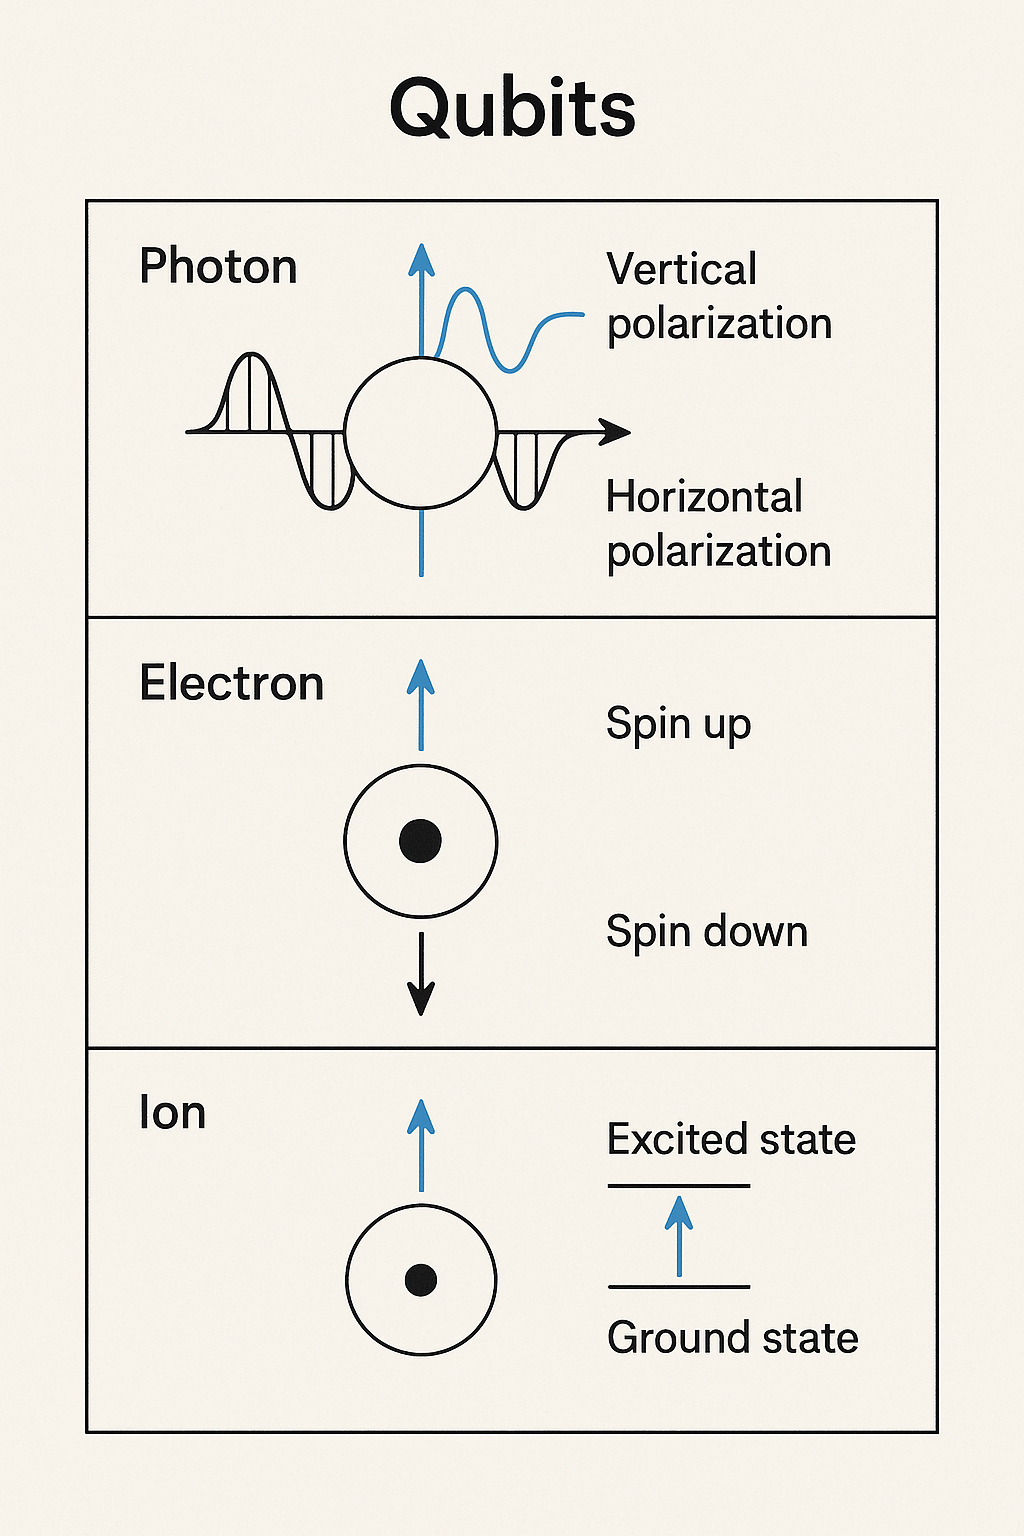
\includegraphics[width=0.3\textwidth, inner]{figures/physical_qubits_2.png}
	\end{adjustbox}
	\caption{Representation of physical qubit states} %\href{https://commons.wikimedia.org/wiki/File:Tolmukapea.jpg}{https://commons.wiki-\\media.org/wiki/File:Tolmukapea.jpg}.}
\label{fig:phys_qubit}
\end{figure}

These simple two level quantum systems have two states that we can label $\lvert0\rangle$ and $\lvert1\rangle$;
"horizontal" or "vertical", "up" or "down", "ground" or "excited".
We can then draw an analogy between a digital bit in a classical computer that has the states $0$ or $1$.
What is different about the information being manipulated in these two systems?
In a digital system we have a switch that we can flip from one state to another.
In quantum systems have something like a hi-fi balance knob that we can have either state,
or a mixed combination of the two.

In this framing, we have an amplitude, $\alpha$ and $\beta$, for each state, 
and the combined particle state is the vector $\lvert\psi\rangle = \alpha \lvert0\rangle + \beta \lvert1\rangle$.
Our system two level quantum system is a \emph{qubit} and it can be in a \emph{superposition} of the two states.

Graphically we can represent the combined state of these two special orthogonal \emph{computational basis states} 
as a point on a unit circle in a regular Euclidean space, which is a generalisation of a \emph{Hilbert space}.  

\begin{figure}[ht] 
	\begin{adjustbox}{center}
		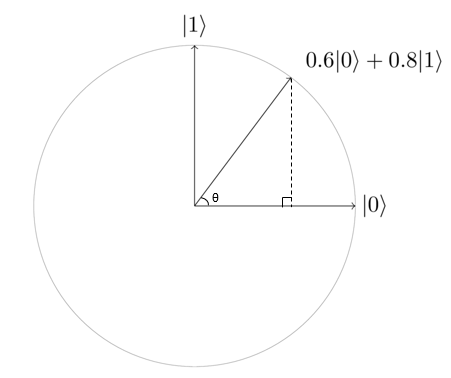
\includegraphics[width=0.3\textwidth, inner]{figures/unit-vector-2-d-hilbert-state.png}
	\end{adjustbox}
	\caption{$\lvert\psi\rangle$ as superposition of $\lvert0\rangle$ and $\lvert1\rangle>$ }
	\label{fig:2d_hilbert_space}
\end{figure}

We can in many cases think of $\alpha$ and $\beta$ as real numbers, but for they complex numbers, 
so this qubit space is described mathematically as a two-dimensional complex 
Hilbert space $\mathcal{H} : \mathbb{C}^2$ \cite{Preskill:2023} \cite{Nielsen:2010}.


%%%%%%%%%%%%%%%%%%%%%%%%%%%%%%%%%%%%%%%%%%%%%%%%%%%%%%%%%%%%%%%%%%%%%%%%%%%%%%%%%%%%%%%%%%%%%%%%%%%%%%%%%%%%%%%%%%%%%%%%
\subsubsection{Probabilistic Measurement}

Once we disturb this state $\lvert\phi\rangle$ by measuring our quantum particle, 
we will either see it in one of these basis states, states that we can measure and observe; 
horizontal or vertical polarization, up or down spin state, high or low energy levels.  

Whilst the system is isolated and unobserved, we can apply transforms, or computations, to the system,
and our qubit can evolve as a point on a sphere of possibilities, until we measure it's state as one of the two basis states;
a photon yielding "horizontal" or "vertical" polarisation.  
The final measurement outcome is inherently probabilistic; 
the probability of measuring $\lvert0\rangle$ is $\lvert\alpha\lvert^2|$, or $\lvert1\rangle$ $\lvert\beta\lvert^2|$.
So these co-ordinates $\alpha$ and $\beta$ have to obey certain rules, 
such as $\lvert\alpha\lvert^2 + \lvert\beta\lvert^2 = 1$; 
the final measurement of our photon guaranteed to be either "horizontal" or "vertical".

Because the $\lvert\alpha\lvert^2 + \lvert\beta\lvert^2 = 1$, we can effectively write our qubit state as \cite{Nielsen:2010}
$$\lvert\psi\rangle = cos \frac{\theta}{2} \lvert0\rangle + e^{i\varphi} sin \lvert1\rangle $$

The numbers $\theta$ and $\varphi$ define a point on a three dimensional \emph{Bloch sphere} 
that is useful initially for visualising a qubit state.

\begin{figure}[ht] 
	\begin{adjustbox}{center}
		\includegraphics[width=0.3\textwidth, inner]{figures/blocksphere-nielsen-and-chuang-toc-and-chapter1-nov00.png}
	\end{adjustbox}
	\caption{Block sphere representation of a qubit }
	\label{fig:block_sphere}
\end{figure}

At later stages these can be developed into an understanding the benefits and difficulties each 
realisation of a quantum system.

%%%%%%%%%%%%%%%%%%%%%%%%%%%%%%%%%%%%%%%%%%%%%%%%%%%%%%%%%%%%%%%%%%%%%%%%%%%%%%%%%%%%%%%%%%%%%%%%%%%%%%%%%%%%%%%%%%%%%%%%
\subsubsection{Matrix Notations and Unitary Transformations}

If we know that the two vectors encoding these two basis states of our vector space are
$$\lvert0\rangle = \begin{bmatrix} 1 \\ 0 \end{bmatrix} \quad \textrm{and} \quad \lvert1\rangle = \begin{bmatrix} 0 \\ 1 \end{bmatrix}$$

then for the mathematically inclined giving the qubit state representation as:

$$\lvert\phi\rangle = \begin{bmatrix} \alpha \\ \beta \end{bmatrix} = \alpha\lvert0\rangle + \beta\lvert1\rangle$$
could be enlightening.

One postulate of quantum mechanics states that the evolution of an isolated system is unitary:
$$ \lvert \psi'\rangle = U \lvert \psi \rangle, \quad U^{\dagger} U = I$$

represents the notion that applying an operator twice leaves us in the initial state.

Unitary gates are therefore \textbf{reversible}, unlike many classical logic gates. [Consider moving Toffoli example here for continuity.]


We will define more exactly what a quantum circuit is, 
but at this point we can understand it from the our general knowledge of classical digital circuits,
transforming electronic states, doing our bidding in the computers that surround us in our daily lives.
Except that we are using quantum machinery to transform quantum states.

One of the postulates of quantum dynamics is that the evolution of a closed quantum system is described by a
\emph{unitary transformation} \cite{Nielsen:2000}.  
Given a state of a system at $t_1$ as $|\psi\rangle$, it is related to the state $|\psi'\rangle$ at time $t_2$ 
by a unitary operator:

$$|\psi'\rangle = U|\psi\rangle$$

Unitary transforms are invertible by their \emph{conjugate transpose} $U^\dag$.  
Applying the conjugate transpose, we end up where we started, 
which is the same as applying the identity matrix $\mathbb{I}$ to our state, leaving the state unchanged:

$$UU^\dag = \mathbb{I}$$

The practical upshot is that all transforms applied to our quantum state $|\psi\rangle$ has to be a unitary transform.
And that every tiny step in an evolving quantum system can be run backwards exactly.

Because of the rules of unitary transformations, at this point, we can imagine our quantum algorithm, or circuit, 
as one large unitary transformation, taking our initial quantum state into our desired final state.


%%%%%%%%%%%%%%%%%%%%%%%%%%%%%%%%%%%%%%%%%%%%%%%%%%%%%%%%%%%%%%%%%%%%%%%%%%%%%%%%%%%%%%%%%%%%%%%%%%%%%%%%%%%%%%%%%%%%%%%%
\subsubsection{Entanglement}

Not all, arbitrary, transformations are valid (irreversible ones especially, and we will touch on that later).
and an application of entanglement in super-dense coding that is a good model to covering ground quickly \cite{Nielsen:2010}

%\href{https://www.forbes.com/sites/chadorzel/2017/02/28/how-do-you-create-quantum-entanglement/}{how-do-you-create-quantum-entanglement}

%%%%%%%%%%%%%%%%%%%%%%%%%%%%%%%%%%%%%%%%%%%%%%%%%%%%%%%%%%%%%%%%%%%%%%%%%%%%%%%%%%%%%%%%%%%%%%%%%%%%%%%%%%%%%%%%%%%%%%%%
\subsubsection{Quantum Registers and Tensor Products}

In quantum computing a \emph{quantum register} is a system of  \cite{Lipton:2021} (p140).


%%%%%%%%%%%%%%%%%%%%%%%%%%%%%%%%%%%%%%%%%%%%%%%%%%%%%%%%%%%%%%%%%%%%%%%%%%%%%%%%%%%%%%%%%%%%%%%%%%%%%%%%%%%%%%%%%%%%%%%%
\subsubsection{Projective measurement, Born rule}


%%%%%%%%%%%%%%%%%%%%%%%%%%%%%%%%%%%%%%%%%%%%%%%%%%%%%%%%%%%%%%%%%%%%%%%%%%%%%%%%%%%%%%%%%%%%%%%%%%%%%%%%%%%%%%%%%%%%%%%%
\subsubsection{Decoherence vs interference}


%%%%%%%%%%%%%%%%%%%%%%%%%%%%%%%%%%%%%%%%%%%%%%%%%%%%%%%%%%%%%%%%%%%%%%%%%%%%%%%%%%%%%%%%%%%%%%%%%%%%%%%%%%%%%%%%%%%%%%%%
\subsubsection{NISQ and FTQC; Fidelity and Quantum Error Correction}

%%%%%%%%%%%%%%%%%%%%%%%%%%%%%%%%%%%%%%%%%%%%%%%%%%%%%%%%%%%%%%%%%%%%%%%%%%%%%%%%%%%%%%%%%%%%%%%%%%%%%%%%%%%%%%%%%%%%%%%%

Limited Information from Measurement: A single measurement of an $n$-qubit state yields only $n$ bits of classical data, 
revealing only a \enquote{meager shadow} of the underlying quantum state \cite{Preskill:2023}.

%%%%%%%%%%%%%%%%%%%%%%%%%%%%%%%%%%%%%%%%%%%%%%%%%%%%%%%%%%%%%%%%%%%%%%%%%%%%%%%%%%%%%%%%%%%%%%%%%%%%%%%%%%%%%%%%%%%%%%%%
\subsubsection{Noise and Decoherence}
%\cite{Morales:2025}


%%%%%%%%%%%%%%%%%%%%%%%%%%%%%%%%%%%%%%%%%%%%%%%%%%%%%%%%%%%%%%%%%%%%%%%%%%%%%%%%%%%%%%%%%%%%%%%%%%%%%%%%%%%%%%%%%%%%%%%%
\subsubsection{Estimating Gates and Circuit Depth}

%\emph{Note: the paper used QISKIT quantum simulator.  The paper has the shot count, but can we see the noise applied?}

%describe shot count; shot noise and statistical error—kernel variance shows up directly in OC-SVM decision boundaries.


%%%%%%%%%%%%%%%%%%%%%%%%%%%%%%%%%%%%%%%%%%%%%%%%%%%%%%%%%%%%%%%%%%%%%%%%%%%%%%%%%%%%%%%%%%%%%%%%%%%%%%%%%%%%%%%%%%%%%%%%
%\subsubsection{Primitives to Support Quantum Kernel Computations}

%Now we look at the quantum kernel computation itself.  
%We are not going to analyse the 

%which often involves measurement techniques like the SWAP test, implied by overlap/fidelity calculations


%%%%%%%%%%%%%%%%%%%%%%%%%%%%%%%%%%%%%%%%%%%%%%%%%%%%%%%%%%%%%%%%%%%%%%%%%%%%%%%%%%%%%%%%%%%%%%%%%%%%%%%%%%%%%%%%%%%%%%%%
\subsection{What Can we take from Shor}

The ubiquity of Shor's algorithm for integer factorisation and finding discrete logarithms,
interestingly means that we need a wide range of supporting methods early.  

Shor implements an existing, classical, Sch\"{o}nhage-Strassen fast multiplication algorithm.
This uses a Fourier transform, to find order of a function.  
When factoring $M = pq$, $p$ and $q$ being distinct prime numbers,
we can define a function $f_x(a) = (x^a mod M)$, which because of the modular arithmetic, is periodic.
That is, given $r' = (p-1)(q-1)$, $x^{a+r'} mod M) = x^a mod M$ because, as p and q are prime, 
from the Chinese Remainder Theorem, $x^{p-1} \equiv 1 mod p$ and  $x^{q-1} \equiv 1 mod q$.
So the function has a minimal period $r$ that divides $r'$.  
To find the smallest integer $r$ such that $x^r = 1 mod M$, 
we show that $f_x(0),..., f_x(r-1)$ are distinct.  
At this point we just need to note that after implementing the modular exponentiation,
Shor uses a $Quantum Fourier Transform$ (QFT) to find the period of the function \cite{Shor:1994}. 

%%%%%%%%%%%%%%%%%%%%%%%%%%%%%%%%%%%%%%%%%%%%%%%%%%%%%%%%%%%%%%%%%%%%%%%%%%%%%%%%%%%%%%%%%%%%%%%%%%%%%%%%%%%%%%%%%%%%%%%%
\subsubsection{Quantum Computing Stages}

Shor's algorithm demonstrates the main quantum computation stages \cite{Nielsen:2010}:

\begin{enumerate}
	\item Data/State preparation: 
	
	\item Unitary transformation/Computation:
	
	\item Measurement: 
	
\end{enumerate}

With integer factorization, it is easy to verity is necessary to boost the probability of success \cite{Lipton:2021}.
Shor's algorithm succeeds with a probability of less than one.


%%%%%%%%%%%%%%%%%%%%%%%%%%%%%%%%%%%%%%%%%%%%%%%%%%%%%%%%%%%%%%%%%%%%%%%%%%%%%%%%%%%%%%%%%%%%%%%%%%%%%%%%%%%%%%%%%%%%%%%%
\subsubsection{Amplitude Amplification}

Like many quantum algorithms, this 
\emph{Amplitude Amplification} (AA) \cite{Dalzell:2023} is the probabilistic technique of 
repeating the call and to a unitary that verifies success of the call, to boost the success probability
closer to 1.

%We have already made the point that quantum computing applies reversible unitary transformations to the quantum state.  
%The modular exponentiation arithmetic is a 

%The technique uses 
%The reversible modular exponentiation 

%So the exponential improvement of  over the classical version is 


%We can view the modular \cite{Dalzell:2023}

This is in contrast to Block-encoding, 
helps define certain ideas that are needed to engage with quantum computing as $C = U_1 .. U_n$. 
The core insight being that classical computing can be realised by quantum machinery, 
not by making the classical computational reversible (boolean functions can be made reversible\cite{Bennett:1989}),
but by admitting that the dynamics of a subsystem with a quantum system can be non-unitary.

%%%%%%%%%%%%%%%%%%%%%%%%%%%%%%%%%%%%%%%%%%%%%%%%%%%%%%%%%%%%%%%%%%%%%%%%%%%%%%%%%%%%%%%%%%%%%%%%%%%%%%%%%%%%%%%%%%%%%%%%
\subsubsection{State Preparation}

Encoding classical data into quantum states efficiently can be non-trivial, 
sometimes requiring circuits whose complexity scales with the classical data size, despite the memory compression in qubits


%%%%%%%%%%%%%%%%%%%%%%%%%%%%%%%%%%%%%%%%%%%%%%%%%%%%%%%%%%%%%%%%%%%%%%%%%%%%%%%%%%%%%%%%%%%%%%%%%%%%%%%%%%%%%%%%%%%%%%%%
\subsection{Investigation into an Application of Quantum Computation}

In a recent paper, \citetitle{Poutre:2024}, \citeauthor{Poutre:2024} \cite{Poutre:2024} use a modified 
\emph{Large Language Model} (LLM) \emph{Transformer} auto-encoder architecture to 
\enquote{learn rich temporal limit order book subsequence representations}.  
From this trained encoder network they then train an OC-SVM to detect financial fraud, with seemingly good results.

A Support Vector Machine (SVM) is a machine learning algorithm used for classification and regression tasks.  
It is widely used in text classification and image recognition, for example.
Typically they are used in a supervised learning context where labelled data is available to fit the model.

The primary aim of the SVM is to separate data points into distinct classes by finding the best boundary that divides them.
In a 2-D space this boundary is a line, in 3-D a plane, and in higher dimensional spaces, a \emph{hyperplane}.
This boundary is found by maximising the distance between the boundary and the nearest data points in each class;
these '\emph{support vectors}' define the hyperplane. 
If the data isn't neatly separable, 
the SVM uses an mathematical transform to project the data into a higher dimensional space, 
where a clear boundary can be found.
These transformations are called \emph{kernels}, and there are many classes of kernels available.

\citeauthor{Scholkopf:1999} in 1999 \cite{Scholkopf:1999} introduced OC-SVMs as a variant of SVMs designed for one task;
outlier or novelty detection.
By focusing on distinguishing between 'normal' data and everything else, 
and only forming a hyperplane using a single class of data during training, 
they can used for semi or un-supervised applications.

\citeauthor{Kyriienko:2022} \cite{Kyriienko:2022} in 2022 developed an application of OC-SVMs using quantum kernels.
In their paper they successfully used a simulator of 20 qubits (one qubit per dataset feature)
on a reduced data set, and most interestingly, performed analysis on the training and inference times needed, 
and in the process demonstrating that the quadratic scaling of the Gram matrix evaluation 
made their approach infeasible on the full dataset.

Promising work has been done to reduce the time-complexity of the evaluation of the Gram matrix, 
by \citeauthor{Kolle:2023} \cite{Kolle:2023}, using randomised measurements and variable subsampling.

The aim of the studedent's paper would be to investigate whether quantum kernel OC-SVM algorithms are practical 
given our reliance of NISQ machinery.
It is well known that these devices have the constraints of having only limited number of qubit to represent model state,
and that they introduce errors that constrain the complexity and depth of circuits that they can run \cite{Preskill:2018}.
In their paper, P\"{o}utre state that their autoencoder of had a dimensionality of 128 \cite{Poutre:2024},
far larger that the feature set of 20 used by Kyriienko \cite{Kyriienko:2022}.
With the recent announcement by Google that their new 105 qubit \emph{Willow} processor has
achieved below threshold quantum error correction \cite{Google:Willow:2024}, the main body of this report is to: 
(1) reanalyse the training and inference times by Kyriienko assuming the performance stated in Google's research;
(2) assess whether the new hardware could be used to apply the OC-SVM algorithm to the P\"{o}utre paper dataset
and to estimate for the training and inference times.


%%%%%%%%%%%%%%%%%%%%%%%%%%%%%%%%%%%%%%%%%%%%%%%%%%%%%%%%%%%%%%%%%%%%%%%%%%%%%%%%%%%%%%%%%%%%%%%%%%%%%%%%%%%%%%%%%%%%%%%%
\subsubsection{Leveraging Classical Competencies}
	
The topic was contrived to demonstrate several points,
one being that delivery of the quantum syllabus should draw on other competencies
that the student and programme curriculum provide.

The student should feel capable of being able to apply the core quantum principals to novel situations.  
The example here is of using a concepts of time and space complexities to estimate quantum computing resources.

Many sources emphasise the importance of "end-to-end" analysis when evaluating quantum \cite{Dalzell:2023} \cite{Morales:2025}
algorithms, including classical and quantum overheads (state preparation, measurement, error mitigation),
to assess the feasibility and potential quantum advantage of these solutions.  
Resource estimation (qubits, gates, runtimes, measurement shots) 
is a key aspect of understanding challenges and limitations,
and hence a desirable outcome for new practitioners.

%%%%%%%%%%%%%%%%%%%%%%%%%%%%%%%%%%%%%%%%%%%%%%%%%%%%%%%%%%%%%%%%%%%%%%%%%%%%%%%%%%%%%%%%%%%%%%%%%%%%%%%%%%%%%%%%%%%%%%%%
\subsubsection{Hybrid Processing Pipelines}

A second point is that details from the paper by \citeauthor{Kyriienko:2022} 
bring up an interesting point that may not be obvious from the abstract. 
Their technique is to apply only the kernel transform using quantum techniques, 
not to generate, or embed, the Gram matrix in a quantum vector state.
The constructing the Gram matrix, as well as the autoencoder, use classic computing systems. 
And as in Shor's original quantum paper on discrete logarithms and factoring \cite{Shor:1994},
this is an example of a hybrid classical-quantum computing system \cite{Preskill:2023}.

There are commercial realities \emph{(and skills shortages anecdotally from workshop I went to)}
that can have direct tie-ins to data engineering skills being developed with the full curriculum.

In this hybrid model, 
the quantum system acts as a co-processor, executing specific sub-routines that are expected to offer quantum advantage.
The classical computer orchestrates data preparation, algorithm set-up, and post-processing tasks.
There are parallels to the engineering challenges of \emph{Extract, Transform, Load} (ETL) 
in classical machine learning data pipelines and GPU workflows.

%%%%%%%%%%%%%%%%%%%%%%%%%%%%%%%%%%%%%%%%%%%%%%%%%%%%%%%%%%%%%%%%%%%%%%%%%%%%%%%%%%%%%%%%%%%%%%%%%%%%%%%%%%%%%%%%%%%%%%%%
\subsubsection{Exposure to Commercial Platforms}

\emph{Commercial offerings are available, so there are options to fold practical experience into the course options.
	Hybrid processing pipelines examples; would need to introduce products (move to a later part of this section on SDKs)}

\begin{itemize}
	\item \href{https://docs.aws.amazon.com/braket/latest/developerguide/braket-what-is-hybrid-job.html}
	{AWS Braket Hybrid jobs}
	\item \href{https://pennylane.ai/qml/demos/tutorial_quantum_transfer_learning}
	{Pennylane hybrid Quantum Transfer Learning example}
	\item \href{https://ml2quantum.com/2020/05/22/zapata-orquestra/}
	{Zapata Orquestra; I haven't looked into yet}
	\item \href{https://docs.quantum.ibm.com/api/qiskit-ibm-runtime/0.16/runtime-service
	}{IBM Qiskit Runtime allows an aspect or orchestration}
\end{itemize}

%%%%%%%%%%%%%%%%%%%%%%%%%%%%%%%%%%%%%%%%%%%%%%%%%%%%%%%%%%%%%%%%%%%%%%%%%%%%%%%%%%%%%%%%%%%%%%%%%%%%%%%%%%%%%%%%%%%%%%%%
\subsubsection{Block Encoding and Quantum Linear System Solvers}

When we were talking about quantum computation first downside of this imposed rule, is that not all, arbitrary, transformations are valid 
(irreversible ones especially, and we will touch on that later).

The pressing problem for machine learning, Gram matrices for SVM kernels, 
Hamiltonian matrices describing a desired evolution, and general data vectors, are generally non-unitary.
If we want to run our Netflix recommender system in our brave new, fully quantum (none of this hybrid rubbish), world,
how do we keep the physics happy, whilst computing the matrix we actually want?

Without going into the details, but typically by introducing additional quantum registers, or \emph{ancillas}, 
there is a more advanced technique called \emph{Block Encoding} (BE) that can embed a, possibly non-unitary, matrix $A$ 
into a larger unitary $U$ \cite{Low:2017}.

$$
U = \begin{bmatrix} A & \ast \\ \ast & \ast \end{bmatrix}
$$

\emph{There is probably not much use here to introduce other precursor 
algorithms, such as the original \emph{Quantum Linear System Solver} (QLSS) by \citeauthor{Harrow:2009} \cite{Harrow:2009},
or to look at the history of block encoding from Berry, Childs, Cleve, Kothari and others, 
showing that you can simulate sparse Hamiltonians by writing them as linear combinations of short unitaries,
or looking at other more wide spread applications \emph{cite 2018 Gilyen, Su, Low \& Wiebe} 
via Quantum Singular Value Transformation (QSVT) 
where they apply lblock encoding with signal processing techniques, developing a single unifying technique} 

\pagebreak

\section{Introduction to Quantum Computing Syllabus Outline}

%\emph{Section 3 then lays out those topics in a forward-flow syllabus,  mapping topics onto specific, measurable learning outcomes.}

%There are many good overviews of where the subject is currently \cite{Preskill:2023}.

%\cite{Abhijith:2022}

%There are also many reviews and surveys on currency algorithm classes \cite{Arnault:2024} \cite{Jordan:2024} 

%\emph{
%	Expound on the problem of the lack of mental models from non-quantum topics (eg universal gates for classical digital computing)
%	that are all students will know.
%	Show that the introduction of certain quantum ideas may require the fore-shadowing (? better term) of classical ideas 
%	that are an analogue or antithesis of the quantum phenomenon (e.g no universal gates in quantum circuits).
%}


%%%%%%%%%%%%%%%%%%%%%%%%%%%%%%%%%%%%%%%%%%%%%%%%%%%%%%%%%%%%%%%%%%%%%%%%%%%%%%%%%%%%%%%%%%%%%%%%%%%%%%%%%%%%%%%%%%%%%%%%
%%%%%%%%%%%%%%%%%%%%%%%%%%%%%%%%%%%%%%%%%%%%%%%%%%%%%%%%%%%%%%%%%%%%%%%%%%%%%%%%%%%%%%%%%%%%%%%%%%%%%%%%%%%%%%%%%%%%%%%%
\subsection{Unit 1: Quantum Foundations and Hardware}\label{sec:U1-outline}

%We present an introduction to the field of quantum computing. 
%We do this by setting out the historic origins and the fundamental concepts that distinguish it from classical computation.
%The unit introduces qubits and quantum gates, and looks briefly at the physical systems used to realise them.
%We aim to build in intuition and background to build the mathematical formalism introduced in subsequent units.

%A gentle introduction seeks to highlight why quantum computation is special.
%By understanding a little about how we create quantum particles and exotic quantum states, 
%the student should feel more confident in the more abstract concepts introduced as the unit progresses.

Learners need a shared vocabulary (qubits, gates and physical realisations) before they can tackle algorithms or cryptographic threats. 
A brief historical sketch and a tour of today's hardware ground the abstract mathematics that follows.

%%%%%%%%%%%%%%%%%%%%%%%%%%%%%%%%%%%%%%%%%%%%%%%%%%%%%%%%%%%%%%%%%%%%%%%%%%%%%%%%%%%%%%%%%%%%%%%%%%%%%%%%%%%%%%%%%%%%%%%%
\subsubsection{Quantum Computing History}

\emph{Purpose}: show that quantum computing arose from the practical question raised by Feynman,  "how do we simulate quantum physics?", 
and evolved through Deutsch to modern NISQ devices.

%This unit draws on Preskill's paper \citetitle{Preskill:2023} \cite{Preskill:2023} (2023)
%and Feynman's \citetitle{Feynman:1986} (1986) \cite{Feynman:1986}, 
%to provide a historical context and initial motivation for quantum computing.

%Feynman introduces intuitively why quantum systems cannot be simulated efficiently by classical computers.
%He does this through the description of analogue simulation of physical quantum systems, 
%and so allows the student so see the contrast with digital quantum information processing with qubits and gates.
%A discussion on Deutsch's contributions - \citetitle{Deutsch:1985} \cite{Deutsch:1985} (1985) - offers context on this.

\emph{Key message}: classical computers struggle to model quantum systems; quantum hardware was conceived to close that gap.


%%%%%%%%%%%%%%%%%%%%%%%%%%%%%%%%%%%%%%%%%%%%%%%%%%%%%%%%%%%%%%%%%%%%%%%%%%%%%%%%%%%%%%%%%%%%%%%%%%%%%%%%%%%%%%%%%%%%%%%%
\subsubsection{The Qubit: Representations and Realizations}

\emph{Purpose}: define the qubit as a two-level quantum system and introduce the vector/Bloch-sphere picture.

%We introduced the qubit by talking about two-level quantum systems.
%Using examples of photons, trapped ions, quantum dots, superconducting quantum systems, 
%introduce the \emph{vector-state} representation and \emph{bloch-spheres}.
%Whilst talking about quantum states, we can introduce \emph{qudits}, such as \emph{qutrits} and \emph{quarts}.
%Drawing from $q$-ary linear code, we demonstrate the higher cardinality of three- and four-level quantum systems,
%and show that there is no loss in expressiveness in using the qubit abstraction.

%Introduce concepts of \emph{superposition}, \emph{no-cloning} and \emph{entanglement} in one and two qubit systems.
%Through this, introduce the \emph{Dirac} notation along side \emph{binary strings} and \emph{vector notation}
%as representations of superposition and entangled states.
%Use vector spaces and bloch spheres as a natural way of understanding a single qubit system.
%Measurement of computational basis states are discussed.

%We can use the introduction, and a high level, to demonstrate how quantum phenomenon can be manifested through physical systems.
%This can be as simple as using a set of polarising filters to see the ?? paradox.  
%The setup for photons to describe entanglement is straight forward, 
%but we can describe technique for ions and highlight how experimental physics is moving the industry forward 
%by reading \href{http://scienceblogs.com/principles/2009/07/07/entanglement-by-accident/}{Monroe on accidental ion entanglement}.

\emph{Key message}: superposition, no-cloning and entanglement distinguish qubits from bits, 
yet all can be expressed in familiar linear-algebra terms. 
Higher-level \emph{qudits} exist but do not expand computational power beyond the qubit abstraction.

%%%%%%%%%%%%%%%%%%%%%%%%%%%%%%%%%%%%%%%%%%%%%%%%%%%%%%%%%%%%%%%%%%%%%%%%%%%%%%%%%%%%%%%%%%%%%%%%%%%%%%%%%%%%%%%%%%%%%%%%
\subsubsection{Quantum Machinery}

\emph{Purpose}: orient students within the hardware landscape; analogue simulators, annealers, photonic devices and gate-based processors.

%Give examples of the major categories of quantum computing:
%\begin{itemize}
%	\item Analogue Quantum\,Simulators; specialised setups to gain insights into strongly correlated matter (condensed-matter models, spin states).
%	\item Analogue QUBO annealers, such as D-Wave: Fixed Ising form solvers with flexibility over in scalar parameters.
%	\item Digital photonics, such as PsiQuantum: single-photon and time-bin approaches, uses in communications.
%	\item Digital gate based systems: typically super-conducting and trapped-ions technologies for general computing applications.
%\end{itemize}

%Examples of where natural advantages of certain technologies, such as photonics for quantum communication 
%and quantum cryptography and key distribution can be discussed.

%Photonics poses interesting challenges and opportunities. 
%Is both one of the earliest \emph{cite{photonics}} practical quantum technologies 
%and an expensive one to set up research for \emph{cite{photonics:costs-of-research}}. 
%Yet it has easily demonstrates a number of quantum principles in a way which is easily explainable at an under-graduate science level.
%Early \emph{Quantum Key Distribution (QKD)}  \index{Quantum Key Distribution} used quantum properties of photons, 
%specifically photon polarisation - which can be demonstrated with polarised sunglasses - to develop the delivery of one-time pads 
%for secure communications.

%Further, the exposition of the QKD of randomly generated one time pads highlights another recent development
%where quantum randomness was demonstrated for the first time recently, using digital quantum computers and RCS
%[\href{https://scitechdaily.com/a-56-qubit-quantum-computer-just-did-what-no-supercomputer-can/}{google jpm 56 qubit QRNG}].

%Looking at the physical implementation of quantum systems, we will see certain advantages of different quantum particles
%with respect to  \emph{noise}, \emph{decoherence} and \emph{gate fidelity}.
%This brings into scope the topics of near-term \emph{NISQ} vs the holy-grail of \emph{FTQC}, 
%laying the ground work for the introduction of quantum error correction schemes.

\emph{Key message}: different technologies excel in different niches 
(e.g. photonics for communications, superconducting qubits for general algorithms), 
and noise considerations motivate the distinction between NISQ and future fault-tolerant machines.

%%%%%%%%%%%%%%%%%%%%%%%%%%%%%%%%%%%%%%%%%%%%%%%%%%%%%%%%%%%%%%%%%%%%%%%%%%%%%%%%%%%%%%%%%%%%%%%%%%%%%%%%%%%%%%%%%%%%%%%%
\subsubsection{Outcomes}
By the end of Unit\,1, students can:
\begin{itemize}
	\item \emph{Explain} Feynman's simulation argument and its significance for quantum computation.
	\item \emph{Contrast} classical and quantum computing using the state-space (exponential) argument.
	\item \emph{Identify} the major hardware platforms and discuss their practical trade-offs.
	\item \emph{Describe} at least one experimental set-up that manifests superposition or entanglement (e.g. polarised photons).
\end{itemize}

\subsubsection{Reference Materials}
\begin{itemize}
	\item \citeauthor{Preskill:2023} \citetitle{Preskill:2023}.
	\item \citeauthor{Feynman:1986} \citetitle{Feynman:1986}.
	\item \citeauthor{Nielsen:2010} \citetitle{Nielsen:2010} ch. 1.
	\item \citeauthor{Lipton:2021} \citetitle{Lipton:2021} ch. 14 (qudits).
	\item \citeauthor{Monroe:2021} \citetitle{Monroe:2021}.
	\item Vendor white papers (D-Wave/quantum annealing), PsiQuantum/photonics, ORCA/fibre optics).
	%\item ORCA White Paper: "Quantum computing using optical fibre components" [ORCA, 2022, company website/documentation]
	\item Light-hearted primer: Chad Orzel, \href{https://chadorzel.com/?cat=4}{How to Teach Physics to Your Dog}.
\end{itemize}

%%%%%%%%%%%%%%%%%%%%%%%%%%%%%%%%%%%%%%%%%%%%%%%%%%%%%%%%%%%%%%%%%%%%%%%%%%%%%%%%%%%%%%%%%%%%%%%%%%%%%%%%%%%%%%%%%%%%%%%%
\subsection{Unit 2: Quantum Computation, Gates and Circuits}

This unit presents the foundational mathematical skill sets needed to describe and apply gates to effect computations. 
Students now translate the physical intuition from Unit\,1 into the mathematical grammar of quantum computing
(linear algebra, postulates, gates and simple circuits) so that every later algorithmic idea has a precise formal scaffold.

%%%%%%%%%%%%%%%%%%%%%%%%%%%%%%%%%%%%%%%%%%%%%%%%%%%%%%%%%%%%%%%%%%%%%%%%%%%%%%%%%%%%%%%%%%%%%%%%%%%%%%%%%%%%%%%%%%%%%%%%
\subsubsection{Linear Algebra}

\emph{Purpose}: supply the indispensable toolkit of vector spaces, inner products, matrix operators and tensor products,
and using the qubit as a running example.

\emph{Learning}:
\begin{itemize}
	\item Express single- and multi-qubit states as column vectors.

	\item Identify Hermitian, unitary and Pauli operators and explain why unitarity $\iff$ reversibility.

	\item Compute simple tensor products and eigen-decompositions with pen-and-paper and NumPy.
\end{itemize}

%We mostly follow \citeauthor{Nielsen:2010} chapter 2 \cite{Nielsen:2010}, 
%but reference other papers where they bring conciseness \cite{Ekert:1996} \cite{Abhijith:2022}.

%We start by recapping single- and dual-qubit vector states, 
%and give the generalization of \emph{quantum registers} used in quantum computing. 

%* Bases and linear independence
%* Linear Operators as Matrices
%* Pauli Matrices
%* Interproducts
%* Eigenvectors and eigenvalues
%* Adjoints and Hermitian Operators:  $U^{\dagger}$ is both the inverse and the transpose-conjugate; multiplying restores  the identity. 
%* Tensor Products
%* Operator functions
%* Commutator and anti-commutator
%* Polar and singular value decompositions

%%%%%%%%%%%%%%%%%%%%%%%%%%%%%%%%%%%%%%%%%%%%%%%%%%%%%%%%%%%%%%%%%%%%%%%%%%%%%%%%%
\subsubsection{Quantum Postulates}

\emph{Purpose}: anchor the algebra to the four standard postulates, 
emphasising Postulates\,2 and\,3 as the dynamical core and Postulate\,4 as the blueprint for composite systems.

\emph{Learning}:
\begin{itemize}
	\item State each postulate in one sentence.
	\item Explain how unitary time evolution and projective measurement coexist.
	\item Give a short explanation of why the Toffoli gate is the reversible AND analogue.
\end{itemize}

%	Most modern texts (e.g., Nielsen \& Chuang) frame non-relativistic quantum mechanics around four core postulates. 
%	Two describe \textbf{states} and \textbf{composite systems}, 
%	while the other two govern \textbf{dynamics} on how a state changes with time or under measurement.
	
%\emph{Foundational Postulates}
%\begin{itemize}
%	\item \textbf{Postulate 1:} A quantum state is a vector in Hilbert space.
%	\item \textbf{Postulate 4:} Composite systems are described by the tensor product of individual system spaces.
%\end{itemize}
	
%These two postulates set the stage, but they do not directly govern dynamical evolution.
	
%	\emph{Postulates Governing Dynamics}
%	\begin{table}[ht]
%		\centering
%		\renewcommand{\arraystretch}{1.2}
%		\begin{tabular}{|c|l|l|l|}
%			\hline
%			\textbf{\#} & \textbf{Postulate} & \textbf{What it says} & \textbf{Why it's “dynamics”} \\
%			\hline
%			\textbf{2. Unitary Time Evolution} & If a system is isolated during the interval $ t_0 \to t $, its state vector evolves by a \textbf{unitary} operator $ U(t,t_0) $. In the Schrödinger picture: & $ U(t,t_0) = \exp\!\bigl[-\,iH(t-t_0)/\hbar\bigr] $, where $ H $ is the system's Hermitian Hamiltonian. & This gives the reversible, deterministic law (Schrödinger equation) for how amplitudes flow; analogous to Newton's laws for classical trajectories. \\
%			\hline
%			\textbf{3. Measurement (Projective Version)} & Measuring an observable $ M $ with eigenvalues $ \{m_k\} $ and projectors $ \{P_k\} $ produces outcome $ m_k $ with probability $ p_k=\langle\psi|P_k|\psi\rangle $. After measurement, the system jumps to: & $ P_k|\psi\rangle/\sqrt{p_k} $. & This is the \textbf{non-unitary} dynamical rule that accounts for interaction with a detector and explains why we observe definite outcomes despite quantum interference. \\
%			\hline
%		\end{tabular}
%		\vspace{4pt}
%		\caption{Postulates governing dynamics in quantum mechanics}
%	\end{table}
%	\emph{Summary}
%	Postulate 2 provides the continuous, reversible evolution between measurements, while Postulate 3 supplies the stochastic, irreversible update during measurement. Together, they form the complete dynamical framework of standard quantum theory.

%Classical irreversible gates: 
%* Show truth table of AND. Ask: can you recover the inputs from the output? No! Information is lost.
%* Introduce the Toffoli gate (adds a third control bit to keep reversibility).

%Qubit and unitarity rule
%* Define qubit $|psi\rangle = \alpha |0\rangle + \beta |1\rangle⟩$.
%* State "Quantum mechanics says evolution is linear and norm-preserving $\Rightarrow$ matrices must be unitary."

%Unitary $\iff$ reversible
%* Prove quickly: $U^\dag$ is both the inverse and the transpose-conjugate; multiplying restores the identity.

%Circuit as factorisation
%* Stack three 2×2 matrices; note the product is still unitary.
%* Draw the same gates in reverse order with daggers = inverse circuit.

%Non-unitary aspirations
%* "We want to multiply by a real-valued data matrix or Hamiltonian; those aren't unitary."

%Block-encoding mechanics
%* Add one ancilla qubit initialised to $|0\rangle$.
%* Show that controlling on the ancilla embeds $A/\alpha$ in the top-left corner of the full matrix.
%* Stress the scaling factor αα and the success-probability interpretation.

%%Teaser of downstream uses
%%* Mention HHL, QSVT, quantum kernels: "All call a block-encoding as a subroutine."
%%* End with the mantra: "Circuits implement unitaries; block-encodings let those unitaries secretly carry the matrices we care about."

%%%%%%%%%%%%%%%%%%%%%%%%%%%%%%%%%%%%%%%%%%%%%%%%%%%%%%%%%%%%%%%%%%%%%%%%%%%%%%%%%
%\emph{Why Irreversibility shows up in practice}
%
%1. Measurement - Projective measurement applies a non-unitary "collapse" operator. 
%Information about the phase relations among amplitudes is discarded, so you cannot un-measure a generic outcome.
%
%2. Open systems / decoherence - Coupling to an environment causes the joint evolution (system + bath) to stay unitary, 
%but the reduced stat0e of the system alone evolves under a completely-positive trace-preserving (CPTP) map, 
%which is generally not invertible. 
%Apparent irreversibility is just the price of ignoring the environment's qubits.
%
%\emph{Superdense Coding}
%
%* Bell states and EPR
%
%\emph{Density Operator}
%
%\emph{Schmidt decomposition and purifications}

%%%%%%%%%%%%%%%%%%%%%%%%%%%%%%%%%%%%%%%%%%%%%%%%%%%%%%%%%%%%%%%%%%%%%%%%%%%%%%%%%%%%%%%%%%%%%%%%%%%%%%%%%%%%%%%%%%%%%%%%
\subsubsection{Basic Gates \& Operations}

\emph{Purpose}: expound on the universal gate set and develop the circuit picture.

\emph{Learning}:
\begin{itemize}
	\item Build a three-gate circuit (e.g. H-CNOT-Z) and predict output probabilities.
	\item Describe the no-cloning theorem's impact on quantum communications.
	\item Run a simple circuit in Qiskit or Cirq and verify results against theory.
\end{itemize}

%\textbf{Concepts Covered}:
%\begin{itemize}
%	\item Bra-ket notation and state representation; a way of writing vectors in a 2-D vector space: $|v \rangle \in \mathbb{C}^2$
%	\index{Bra-ket Notation}
%	\item Matrix transformations of quantum states and gates
%	\item Basic gates: Pauli (X, Y, Z), Hadamard (H), CNOT, Phase shifts, and controlled gates
%	\item Principle of reversibility: quantum operations as unitary transformations, implications for circuit construction, contrast to classical irreversibility.
%	\item No-Cloning theorem: proofs and intuitive reasoning, consequences for quantum communication and cryptography.
%\end{itemize}


%\textbf{Workshops}:
%\begin{itemize}	
%	\item IBM Qiskit (core gate library, interactive circuit composer)
%	\item Google Cirq (custom gate implementation, visualizations)
%\end{itemize}

%\begin{itemize}
%	\item Original no-cloning paper: Wootters \& Zurek, "A Single Quantum Cannot Be Cloned," Nature, 1982, doi:10.1038/299802a0
%	\item Explanation of reversibility: \citeauthor{Nielsen:2010}, Quantum Computation and Quantum Information (Chapter 4, sections on unitarity and reversibility).
%\end{itemize}

%%%%%%%%%%%%%%%%%%%%%%%%%%%%%%%%%%%%%%%%%%%%%%%%%%%%%%%%%%%%%%%%%%%%%%%%%%%%%%%%%%%%%%%%%%%%%%%%%%%%%%%%%%%%%%%%%%%%%%%%
\subsubsection{Tensor Mathematics and Circuit Composition}

\emph{Purpose}: show how small gates scale to multi-qubit registers via tensor products and controlled operations.

\emph{Learning}:
\begin{itemize}
	\item Rewrite a controlled-U gate as a block matrix.
	\item Decompose a two-qubit gate into single-qubit rotations and CNOTs (by lookup or SDK).
\end{itemize}

%\textbf{Workshop SDKs/Platforms}:
%\begin{itemize}
%	\item IBM Qiskit Composer (interactive drag-and-drop circuit composer)
%	\item Google Cirq tutorials (introductory lab exercises)
%	\item Julia QML/Yao.jl; automatic differentiation (fast simulations, tensor-network circuits, tensor operations)
%	\item Pennylane: automatic differentiation  (tensor circuit building, differentiable programming)
%\end{itemize}


%%%%%%%%%%%%%%%%%%%%%%%%%%%%%%%%%%%%%%%%%%%%%%%%%%%%%%%%%%%%%%%%%%%%%%%%%%%%%%%%%%%%%%%%%%%%%%%%%%%%%%%%%%%%%%%%%%%%%%%%
\subsubsection{NISQ Devices and Error Correction Codes}

\emph{Purpose}: connect the perfect matrix circuit model to noisy hardware and introduce the idea of logical (encoded) qubits.

\emph{Learning}:
\begin{itemize}
	\item Simulate a bit-flip error and show how a three-qubit repetition code detects it.
	\item Articulate the difference between NISQ error-mitigation and full fault tolerance.
	\item Discuss the practical trade-offs of state preparation on-chip versus hybrid classical-quantum approaches in the NISQ era.
\end{itemize}

%We recap the NISQ devices introduction from Preskill and look at error correction.
%We describe the use of logical qubits constructed from physical qubits. 
%We follow this will quantum error correction to demonstrate theoretical and practical solutions to noise and decoherence.
%Surface and colour stabiliser codes can be explained diagrammatically (hence topological protection),
% and as well as demonstrating on paper how single phase-flip and bit flip errors can be caught an corrected, 
% we can demonstrate this using SDKs.


%\textbf{Workshop SDKs/Platforms}:

%\begin{itemize}
%	\item IBM Quantum Experience (real-device demonstrations, noise simulations)
%	\item Google Cirq (customizable noise models)
%\end{itemize}

%\begin{itemize}
%	\item IBM Qiskit Noise Simulator (interactive noise examples)
%	\item IBM Qiskit Ignis (specialized quantum error correction toolkit)
%	\item Google Cirq (topological code simulations, custom circuit design)
%	\item (Additional tool): Stim (Google's specialized quantum error correction simulator)
%\end{itemize}



%%%%%%%%%%%%%%%%%%%%%%%%%%%%%%%%%%%%%%%%%%%%%%%%%%%%%%%%%%%%%%%%%%%%%%%%%%%%%%%%%
\subsubsection{Outcomes}
By the end of Unit\,2, students can:
\begin{itemize}
	\item \emph{Represent} quantum states in bra-ket, column-vectors, Bloch-sphere co-ordinates form.
	\item \emph{Apply} single- and two-qubit unitary gates and compute resulting state vectors.
	\item \emph{Explain} the four quantum postulates and illustrate each with a direct example.
	\item \emph{Assemble} and run a short circuit on a cloud simulator, interpreting the measurement statistics.
	\item \emph{Demonstrate} how a simple error-correction code protects against a single-qubit error.	
\end{itemize}

\subsubsection{Reference Materials}
\begin{itemize}
	\item \citeauthor{Nielsen:2010} \citetitle{Nielsen:2010}, ch. 2.
	\item Watrous, J. 2018, "The Theory of Quantum Information", ch. 2 (concise linear-algebra review)
	\item Wootters \&\,Zurek, "A Single Quantum Cannot Be Cloned," Nature,\,1982. %Wootters \& Zurek, "A Single Quantum Cannot Be Cloned," Nature, 1982, doi:10.1038/299802a0
	\item IBM\,Qiskit, Google\,Cirq \& Pennylane tutorials for hands-on practice.
	\item \citeauthor{Abhijith:2022} \citetitle{Abhijith:2022}
	\item \citeauthor{Ekert:1996} \citetitle{Ekert:1996}
\end{itemize}

%%%%%%%%%%%%%%%%%%%%%%%%%%%%%%%%%%%%%%%%%%%%%%%%%%%%%%%%%%%%%%%%%%%%%%%%%%%%%%%%%
%%%%%%%%%%%%%%%%%%%%%%%%%%%%%%%%%%%%%%%%%%%%%%%%%%%%%%%%%%%%%%%%%%%%%%%%%%%%%%%%%
\subsection{Unit 3: Quantum Algorithms and Classical Cryptography}

Students now see why quantum computing matters to cryptography:
a handful of core algorithms, most famously Shor's and Grover's, break or undermine real-world protocols. 
This cements the linear-algebra skills from Unit\,2 and prepares students for the algorithmic blocks used in Unit\,4.

%Use Shor's original paper as a motivating example for the ideas that were perfected subsequent to his paper:
%\begin{itemize}
%	\item Period finding as Quantum algorithm
%	\item Modular arithmetic as state preparation
%	\item Quantum phase estimation for modular multiplication and exponentiation 
%	\item Hidden Subgroup Problem in terms a eigenvalue (or phase) of a unitary operator
%	\item The unitary as an Oracle-like Component
%	\item Amplitude Amplification
%\end{itemize}

%We then look at some subsequent algorithms that developed these ideas, building confidence with circuit complexity in preparation for more
%complex building blocks and algorithms in unit-4.


%%%%%%%%%%%%%%%%%%%%%%%%%%%%%%%%%%%%%%%%%%%%%%%%%%%%%%%%%%%%%%%%%%%%%%%%%%%%%%%%%
\subsubsection{Classical Cryptography Problems}

\emph{Purpose}: Review the number theory tasks (factorisation, discrete logs, subset-sum) 
that underpin certain cryptographic protocols, so that the impact of quantum-speed-ups is clear.

%sUnderstand the mathematical underpinnings of hidden-subgroup problems, and their broader application.

%%%%%%%%%%%%%%%%%%%%%%%%%%%%%%%%%%%%%%%%%%%%%%%%%%%%%%%%%%%%%%%%%%%%%%%%%%%%%%%%%
\subsubsection{Deutsch-Jozsa and Simon's Algorithms}

\emph{Purpose}: introduce the hidden-subgroup paradigm in its simplest forms; 
students practise reading small circuits and interpreting their algebraic output.


%%%%%%%%%%%%%%%%%%%%%%%%%%%%%%%%%%%%%%%%%%%%%%%%%%%%%%%%%%%%%%%%%%%%%%%%%%%%%%%%%
\subsubsection{Grover's Algorithm}

\emph{Purpose}: contrast \emph{amplitude-amplification} (AA) speed-ups with exponential ones; 
reinforce oracles, reflection operators and the role of noise in NISQ devices.

%We present a Grover notebook using IBM QISKIT to demonstrate building the unitary Oracle
%and running this with the built in \emph{Grover Operator}.

%We take the opportunity to use noisy backend simulators to observer the effects of noise.

%%%%%%%%%%%%%%%%%%%%%%%%%%%%%%%%%%%%%%%%%%%%%%%%%%%%%%%%%%%%%%%%%%%%%%%%%%%%%%%%%
\subsubsection{Quantum Phase Estimation (QPE) and modular arithmetic}

\emph{Purpose}: show that QPE is the work-horse subroutine behind Shor and many later algorithms; 
modular multiplication provides the concrete oracle.

%\textbf{Workshop SDKs/Platforms}:
%\begin{itemize}
%	\item IBM Qiskit (QFT tutorials, modular exponentiation implementations)
%	\item Pennylane (QFT example notebooks)
%\end{itemize}

%%%%%%%%%%%%%%%%%%%%%%%%%%%%%%%%%%%%%%%%%%%%%%%%%%%%%%%%%%%%%%%%%%%%%%%%%%%%%%%%%
\subsubsection{Quantum Fourier Transform (QFT)}

\emph{Purpose}: link the Fourier basis to period-finding 
and demonstrate a compact circuit that students can simulate.

%Understand QFT, the Fourier basis using qubit representations. Demonstrate using Fourier basis and transform for arithmatic.

%%%%%%%%%%%%%%%%%%%%%%%%%%%%%%%%%%%%%%%%%%%%%%%%%%%%%%%%%%%%%%%%%%%%%%%%%%%%%%%%%
\subsubsection{Putting it all Together with Shor's Algorithm}

\emph{Purpose}: assemble the earlier blocks 
(state preparation, modular arithmetic, QFT)
into the complete quantum attack on RSA.

%\textbf{Workshop SDKs/Platforms}:
%\begin{itemize}
%	\item IBM Qiskit (detailed practical implementations, interactive tutorials)
%	\item Pennylane (modular arithmetic circuits)
%\end{itemize}


%%%%%%%%%%%%%%%%%%%%%%%%%%%%%%%%%%%%%%%%%%%%%%%%%%%%%%%%%%%%%%%%%%%%%%%%%%%%%%%%%
\subsubsection{Outcomes}

By the end of Unit\,3, students can:
\begin{itemize}
	\item \emph{Explain} how Shor's and Grover's algorithms threaten current public-key and symmetric schemes.

	\item \emph{Map} each algorithm to its core building blocks (state preparation, oracle, QFT/QPE, amplitude amplification).

	\item \emph{Implement} a small instance of Shor's or Grover's algorithm on a simulator and interpret the results.

	\item \emph{Discuss} the practical trade-offs of state preparation on-chip versus hybrid classical-quantum approaches in the NISQ era.
\end{itemize}

%\begin{itemize}
%	\item describe intuitively the problems of state preparation
%	\item look at the trade-off of computing states internally on a quantum system vs hybrid classical-quantum system, and the difficulties the NISQ bring to this.
%\end{itemize}

\subsubsection{Reference Materials}
\begin{itemize}
	\item \citeauthor{Lipton:2021} \citeauthor{Lipton:2021}, ch x, y, \& z.
	\item \citeauthor{Nielsen:2010} \citeauthor{Nielsen:2010}
	\item \citeauthor{Shor:1997} \citetitle{Shor:1997}
	\item \citeauthor{Grover:1996} \citetitle{Grover:1996}
\end{itemize}

%%%%%%%%%%%%%%%%%%%%%%%%%%%%%%%%%%%%%%%%%%%%%%%%%%%%%%%%%%%%%%%%%%%%%%%%%%%%%%%%%%%%%%%%%%%%%%%%%%%%%%%%%%%%%%%%%%%%%%%%
%%%%%%%%%%%%%%%%%%%%%%%%%%%%%%%%%%%%%%%%%%%%%%%%%%%%%%%%%%%%%%%%%%%%%%%%%%%%%%%%%%%%%%%%%%%%%%%%%%%%%%%%%%%%%%%%%%%%%%%%
\subsection{Unit 4: Advanced Quantum Algorithms}

Having mastered core algorithms, students now meet the techniques that dominate current research
(matrix inversion, polynomial singular-value transforms, quantum optimisation and hybrid workflows)
so they can read, reproduce and extend state-of-the-art results:

\subsubsection{Quantum Matrix Inversion (with HHL)}

\emph{Purpose}: show how a quantum computer can invert a sparse, well-conditioned matrix
 exponentially faster than classical algorithms, subject to data-loading and read-out caveats.
 
%The Harrow-Hassidim-Lloyd (HHL) \cite{Harrow:2009} \cite{Lipton:2021} algorithm is an important piece of work, 
%designed to solve the Quantum Linear System Problem (QLSP). 
%QLSP can be understood by considering the classical Linear System Problem (LPS) where we seek a vector $x$
%to satisfy the set of linear equations $Ax = b$.  QLSP takes  a sparse, well-conditioned matrix  $A$ 
%and vector $b$, encoded as quantum states, and produces a quantum state $\lvert x\rangle$ as a solution.  
%Solving this problem requires a quantum matrix inversion, which HHL provides.

%This algorithm, although seminal, leaves a number of challenges to overcome before the quantum speed-up of the 
%matrix inversion can be taken advantage of.  The first is that recovering the full classical description of the 
%vector $x$ from the quantum state can be computationally expensive and add significant overhead.

%The second we raise is the problem of \emph{Quantum Random Access Memory} (QRAM) 
%and practical issues in providing fast QRAM and loading large amounts of classical data.  
%This subject comes up in another advanced technique, block encoding.

%%%%%%%%%%%%%%%%%%%%%%%%%%%%%%%%%%%%%%%%%%%%%%%%%%%%%%%%%%%%%%%%%%%%%%%%%%%%%%%%%%%%%%%%%%%%%%%%%%%%%%%%%%%%%%%%%%%%%%%%
\subsubsection{Block Encoding \& Quantum Singular-Value Transformation (QSVT)}

\emph{Purpose}: present block encoding as the universal trick for hiding non-unitary matrices inside unitaries, 
and QSVT as the "polynomial filter" that subsumes Grover, Hamiltonian simulation and HHL.

%We take a high-level approach to QSVT as it is mathematically challenging to present, involving Chebyshev polynomials,
%quantum signal processing and a good amount of linear-algebra bookkeeping.

%The core idea \emph{Block-Encoding} (BE) is that, if you can hide a non-unitary matrix $A$ inside of a matrix 
%This core technique of BE comes up a lot in modern quantum algorithms, and it should be presented.  
%Building on the concepts from Grover's AA, QPE, and Hamiltonian simulation, we present the motivation 
%and the pattern of the solution.  
%Indeed, the analogy of the QSVT as a digital filter acting on frequency components, should bolster earlier work with phases.

%\emph{Outcome}:
%\begin{itemize}
%	\item Understand QSVT as polynomial singular-value transformations via controlled phase sequences.
%	\item Identify Grove and Hamiltonian simulation as special cases.
%	\item Describe an \emph{unitary control register} as block-encoding \emph{plus} an ancilla qubit.
%	\item Run a prepared QSVT circuit on a toy, low-degree, matrix and verify the singular values.
%\end{itemize} 

%%%%%%%%%%%%%%%%%%%%%%%%%%%%%%%%%%%%%%%%%%%%%%%%%%%%%%%%%%%%%%%%%%%%%%%%%%%%%%%%%
\subsubsection{Quantum Optimisation Pathways}

\emph{Purpose}: the current focus has shifted towards heuristic algorithms, inspired by classical principles and quantum phenomena, 
like the \emph{Quantum Approximate Optimization Algorithm} (QAOA) and \emph{Variational Quantum Eigensolver} (VQE).
These heuristic methods are designed for NISQ devices, and lack provable guarantees but hold promise for practical applications.
 
\begin{table}[ht]
	\centering
	%\renewcommand{\arraystretch}{1.2}
	\begin{tabular}{|p{4cm}p{10.25cm}|}
		\hline
		\textbf{Sub-topic} & \textbf{} \\
		\hline
		\textbf{Quantum Annealing \& QUBO (D-Wave)} & Demonstrates hardware tailored to Ising/optimization problems and contrasts analogue with gate-model approaches. \\
		\hline
		\textbf{Gate-model Optimisation (QAOA / VQE)} & Shows how variational circuits tackle the same problems on NISQ gate-based devices. \\
		\hline
		\textbf{Graph Algorithms} & Concrete optimization tasks (Max-Cut, colouring) that map neatly to both annealing and QAOA. \\
		\hline
	\end{tabular}
	\vspace{4pt}
	\caption{Comparison of Quantum Optimization Techniques}
\end{table}

%\textbf{Workshop SDKs/Platforms}:
%\begin{itemize}
%	\item Pennylane (smooth classical-to-quantum transition tutorials)
%	\item Julia QML/Yao tutorials (high-performance QML simulations)
%\end{itemize}
%%%%%%%%%%%%%%%%%%%%%%%%%%%%%%%%%%%%%%%%%%%%%%%%%%%%%%%%%%%%%%%%%%%%%%%%%%%%%%%%%
%\subsubsection{Quantum Annealing and D-Wave Systems}

%\textbf{Workshop SDKs/Platforms}:

%\begin{itemize}
%	\item D-Wave Leap (Quantum annealing experiments, practical QUBO solutions)
%\end{itemize}


%%%%%%%%%%%%%%%%%%%%%%%%%%%%%%%%%%%%%%%%%%%%%%%%%%%%%%%%%%%%%%%%%%%%%%%%%%%%%%%%%
%\subsubsection{Quantum Unconstrained Binary Optimization (QUBO)}

%We introduce Ising and QUBO models for quantum annealing.  
%Problems that are typically tackled with theses models are discussed, 
%principally optimisation problems, Hamiltonians, and energy landscapes of quantum chemistry.

%\textbf{Workshop SDKs/Platforms}:
%\begin{itemize}
%	\item D-Wave Leap platform (directly implement optimization problems)
%	\item Pennylane (variational quantum algorithms for optimization)
%	\item Google Cirq (QAOA tutorials)
%\end{itemize}


%%%%%%%%%%%%%%%%%%%%%%%%%%%%%%%%%%%%%%%%%%%%%%%%%%%%%%%%%%%%%%%%%%%%%%%%%%%%%%%%%
%\subsubsection{Quantum Algorithms for Graph Problems}

%* Graph coloring
%* max-cut
%* shortest path problems

%\textbf{Workshop SDKs/Platforms}:

%\begin{itemize}
%	\item Google Cirq (QAOA for MaxCut, detailed graph problems examples)
%	\item D-Wave Leap (Ising models, graph optimization problems)
%\end{itemize}


%%%%%%%%%%%%%%%%%%%%%%%%%%%%%%%%%%%%%%%%%%%%%%%%%%%%%%%%%%%%%%%%%%%%%%%%%%%%%%%%%
\subsubsection{Quantum Machine Learning (QML)}

\emph{Purpose}: connect kernel methods and variational classifiers to practical anomaly detection (OC-SVM), 
illustrating a full hybrid workflow from data encoding to classical post-processing.

%\emph{ML Primer}
%\begin{itemize}
%	\item Kernels
%	\item SVM math
%	\item Anomaly-detection metrics
%\end{itemize}

%\emph{Quantum Kernels \& Feature Maps}
%\begin{itemize}
%	\item Swap-test
%	\item Fidelity estimation
%	\item Expressivity vs noise
%\end{itemize}

%\emph{ Quantum OC-SVM Workflow}
%\begin{itemize}
%	\item Data-encoding circuits
%	\item Kernel-matrix build on hardware (QVM or real)
%	\item Classical QP (CVXOPT / LIBSVM) for support vectors
%	\item Hybrid inference loop; noise-mitigation hacks
%\end{itemize}

%\emph{Variational Classifiers \& Quantum Neural Nets}
%
%\emph{Hands-on Lab 3}
%\begin{itemize}
%	\item Pennylane (best QSVM wrappers)
%	\item Julia QML for high-performance simulations
%	\item Implement OC-SVM in Pennylane
%	\item Test against classical scikit-learn
%\end{itemize}

%\begin{itemize}
%	\item Pennylane (core QML package, variational circuits, quantum neural nets)
%	\item Julia Quantum ML/QML.jl (efficient QML experiments, classical-quantum hybrid models)
%	\item TensorFlow Quantum (Cirq-based, optional for broader ML integrations)
%\end{itemize}

%%%%%%%%%%%%%%%%%%%%%%%%%%%%%%%%%%%%%%%%%%%%%%%%%%%%%%%%%%%%%%%%%%%%%%%%%%%%%%%%%
\subsubsection{Hybrid Classical-Quantum Systems}

\emph{Purpose}: teach students to treat the QPU as a remote accelerator within 
a larger data pipeline, mirroring how real projects are executed in the NISQ era.

%Unit treats a quantum device as a remote accelerator via hybid-jobs api.
%Exercises reinforce core quantum ideas; state preparation, measurement statistics, error mitigation.

%The analogy: similarly to GPU or ML cloud resources (PyTorch, AWS SageMaker) 
%quantum processes are an external call from the Python code to accelerate 
%an specific loop, while local processing handles the data wrangling, optimisation, logging, etc.

%\begin{itemize}
%	\item rationale behind the use of hybrid classical-quantum computing in the NISQ era
%	\item Swap test; measurement statistics
%	\item Error mitigation
%	\item error budgets
%	\item Parameter-shift rule; unitarity	
%\end{itemize}

%\emph{diagram: loop of [ ETL/Feature engineer -> circuit generation/SDK -> Quantum execution (QPU/sim)]}

%\textbf{Topics}
%\begin{itemize}
%	\item Kernel estimation: OC-SVM kernel loop
%	\item Variational Quantum Algorithms (VQAs) workflows: 
%	Frame VQAs (like QAOA or VQE) as prime examples of the hybrid paradigm, 
%	highlighting the classical optimisation loop and the quantum circuit execution/measurement step; 
%	VQE or QAOA on Braket Hybrid Jobs; 
%	\item Data pipeline walk through ETL-to-QPU pipeline
%\end{itemize}

%\textbf{Outcomes}
%\begin{itemize}
%	\item Architect a pipeline that ingests classical time-series, invokes a quantum kernel routine, and performs classical optimisation.
%	\item Quantify shot noise and latency, choosing batch sizes and iteration counts that respect cloud-QPU quotas.
%	\item Deploy a simple hybrid job on either AWS Braket or IBM
%	\item Classic/Quantum performance 
%\end{itemize}


%%%%%%%%%%%%%%%%%%%%%%%%%%%%%%%%%%%%%%%%%%%%%%%%%%%%%%%%%%%%%%%%%%%%%%%%%%%%%%%%%
\subsubsection{Learning}

By the end of Unit\,4, students can:
\begin{itemize}
	\item \emph{Explain} the high-level steps of HHL and identify its data-loading bottlenecks.
	
	\item \emph{Describe} block encoding and state how QSVT extends Grover and Hamiltonian simulation.
	
	\item \emph{Choose} an appropriate optimisation strategy (annealer vs\,QAOA) for a given QUBO or graph problem.
	
	\item \emph{Implement} a simple quantum kernel OC-SVM on a cloud platform and benchmark against a classical baseline.
	
	\item \emph{Architect} a hybrid workflow that balances shot cost, latency and classical compute.
\end{itemize}

\subsubsection{Reference Materials}
\begin{itemize}
	\item \citeauthor{Lipton:2021} \citetitle{Lipton:2021}
	\item \citeauthor{Harrow:2009} \citetitle{Harrow:2009}
	\item \citeauthor{Abhijith:2022} \citetitle{Abhijith:2022}
	\item \citeauthor{Dalzell:2023} \citetitle{Dalzell:2023}
	\item Low \&\,Chuang, "Hamiltonian Simulation by Uniform Spectral Amplification" (for block encoding).
	\item Farhi et\,al., "A Quantum Approximate Optimization Algorithm."
	\item \citeauthor{Havlicek:2019} \citetitle{Havlicek:2019}
\end{itemize}

(Hands-on: D-Wave\,Leap docs, AWS\,Braket hybrid jobs, Qiskit\,Runtime, PennyLane QSVT demo notebooks.)

\subsection{Quantum SDKs and Platforms}

As we have walked through the syllabus, we have elided the quantum SDK platforms relevant for each topic.
Here is a summary of the systems that are either easily installed to run local and cloud based simulations, 
access real quantum hardware, or used for circuit analysis in our subject areas.

\begin{table}[ht]
	\centering
	%\renewcommand{\arraystretch}{0.2}
	\begin{tabular}{|p{2.8cm}|p{7cm}|p{4cm}|}
		\hline
		\textbf{SDK / Platform} & \textbf{Primary Strength} & \textbf{Ideal Course Sections} \\
		\hline
		IBM Qiskit & Most beginner-friendly; rich gate-model library and free cloud back-ends. & Units\,1-3 (foundations, gates, Shor/Grover labs) \\
		\hline
		Google Cirq & Highly customisable circuits with strong pedagogical resources; integrates with TensorFlow\,Quantum. & Units\,2-4 (intermediate algorithms, QAOA, QML) \\
		\hline
		Pennylane & Native hybrid workflows and automatic differentiation for variational circuits.L & Unit\,4 (QSVT demo, OC-SVM lab) \\
		\hline
		D-Wave Leap & Turn-key quantum annealer for Ising / QUBO optimisation. & Unit\,4 (annealing and graph-optimisation topics) \\
		\hline
		ORCA  & Photonic hardware case studies for communications and QKD. & Unit\,1 (hardware landscape) \\
		\hline
		Julia QML / Yao.jl & High-performance simulation and research-grade QML tooling. & Unit\,4 (advanced QML experiments) \\
		\hline
	\end{tabular}
	\vspace{4pt}
	\caption{Comparison of SDKs for Quantum Computing}
	\label{tab:quantum_sdk_comparison}
\end{table}

\subsection{Syllabus Statement}

This section completes the high-level overview of our course syllabus. 
Appendix A gives a detailed description of each unit's topics, background information, resources 
and suggested laboratory exercises on different various quantum platforms.  

Appendix B contains python notebooks for several unit sections, with full tuition materials 
and practical exercises for students. 
\pagebreak

%\section{Outreach}

Section 4 reviews the out-reach with the (NQCC) and quantum industry.


\begin{table}[!ht]
        \caption{Outreach to Quantum Groups.}
        \centering
        \begin{tabular}{| p{2.0cm} || l l c |}
          %\toprule
          \hline
          Institution & \multicolumn{3}{ l|}{Website} \\
          %\cmidrule(r){2-4}
                      & Person & Technology & Connected \\
          \hline %\midrule
          NQCC  & \multicolumn{3}{l |}{\small{https://}} \\
                & &        & No \\
          IBM   &	\multicolumn{3}{l |}{\small{https://quantumzeitgeist.com/exploring-quantum-computing-with-ibms-qiskit}} \\
                & & QISKIT & No \\
          IONQ  & \multicolumn{3}{l |}{https://ionq.com/} \\
                & &        & No \\
          DWave & \multicolumn{3}{l |}{https://www.dwavesys.com/learn/training/} \\
                & &        & No \\
          \hline %\bottomrule
        \end{tabular}
        \label{tab:distcounts}
\end{table}
\subsection{Outreach}

%\pagebreak

%%%%%%%%%%%%%%%%%%%%%%%%%%%%%%%%%%%%%%%%%%%%%%%%%%%%%%%%%%%%%%%%%%%%%%%%%%%%%%%%%%%%%%%%%%%%%%%%%%%%%%%%%%%%%%%%%%%%%%%%
\section{Project Reflection}

The development of this paper has been quite intricate.  
%An implied assertion of this paper that learning quantum computing techniques 
%is both rewarding and not as difficult as may be supposed.
It rests on the assertion that learning quantum‑computing techniques 
is not only rewarding, but less forbidding than commonly assumed.
My experience, as my own understanding of quantum information and computation matured during this project, 
has reinforced this view; although pulling together a coherent teaching plan has been a challenge.

Three realisations have helped crystallise the final approach and content:
\begin{enumerate}
\item \emph{Make background assumptions explicit}: 
During the delivery of a tutorial on single qubit transforms and their related gates,
when noting that any arbitrary unitary operator can be decomposed 
into a set of single-qubit gates plus the two-qubit controlled-NOT (CNOT) gate \cite{Nielsen:2010},
the analogy failed when I compared this to the universality of NAND and NOR gates 
in the construction of classical logic gates \cite{Wikipedia:UniversalLogicGates}.
It demonstrated to me that the introduction material needs to be self-contained,
supplying all foundational material.

\item \emph{Practising what I preach}: This fed into the realisation that, 
although the paper advocates Outcome‑Based Teaching and Learning (OBTL), 
I wasn't embracing this, centring on content not outcomes.  
This realisation helped reorient both the tutorial content to focus on explicit learning objectives,
and to simplify the syllabus outline to become a clear map from foundations to the programme goal \cite{Wong:2011}.

\item \emph{Shor as a centrepiece}: Whilst refactoring all the material that I'd collected, 
that second realisation allowed me to see that one of those earliest papers, by Peter Shor, 
embodied many core quantum building blocks that later research generalised and developed into new and exciting techniques. 
Shor (along with Grover) also provides natural talking points for hybrid computing, the limitations of NISQ devices, 
and architectural decisions taken when delivering end-to-end quantum solutions.  
Shor's integer factorisation algorithm, itself, becomes an analogue for more advanced quantum computing techniques
and centrepiece for an introductory programme.
\end{enumerate}
\pagebreak

%%%%%%%%%%%%%%%%%%%%%%%%%%%%%%%%%%%%%%%%%%%%%%%%%%%%%%%%%%%%%%%%%%%%%%%%%%%%%%%%%%%%%%%%%%%%%%%%%%%%%%%%%%%%%%%%%%%%%%%%
\section{Conclusion}

This project set out to demonstrate that an outcome-based syllabus,
using both cloud based quantum hardware and local quantum simulators,
can fast-track students of cryptography, data science and applied mathematics
from zero exposure to genuine quantum-computing competence. 

The project structured the curriculum around clearly defined learning outcomes, 
developing mathematical chops, and anchoring the material in the well-understood building blocks 
of Shor's algorithm.  
We demonstrated a coherent teaching pathway that is deliverable with today's SDKs and hardware access.

The pilot with a small cohort of students indicates that scaling the material into a 
full programme is both feasible and worthwhile. 
The next phase is to develop the material further to deliver a complete education programme.

%There is futher work required to develop the actual lesson materials from the syllabus, 
%and we believe that this a worthwhile and meaningful body of work to undertake.

%\begin{quote}\itshape
%\textbf{\emph{Objective}}

%To summarize the findings, discuss the overall success of the project in achieving the stated learning outcomes, 
%and suggest directions for future work. 

%This section should provide a cohesive closing statement on the project's contribution to quantum computing education.

%\textbf{\emph{How to Achieve This}}

%\emph{Summarize Key Findings}: Recap the main achievements, including the effectiveness of the lesson plan in delivering 
%the learning outcomes and the value of the comparative analysis for educational purposes.

%\emph{Evaluate Success in Meeting Objectives}: Assess how well the project met its objectives, using evidence from 
%the roadmap and feedback analysis. Highlight specific skills students gained and areas where the lesson plan proved particularly impactful.

%\emph{Propose Future Directions}: Suggest ways the curriculum could be expanded or adapted for different audiences, such as 
%undergraduates or industry professionals. Discuss potential updates to the lesson plan to reflect new advancements in quantum computing.

%\textbf{\emph{Challenges}}

%\emph{Articulating the Project's Impact}: Clearly communicate the educational impact and significance of the project. 
%Avoid overstating conclusions by focusing on measurable outcomes and evidence gathered.

%\emph{Identifying Meaningful Future Work}: Quantum computing is a rapidly evolving field, so outlining realistic 
%and meaningful future directions requires careful consideration of emerging trends and advancements.
%\end{quote}\ignorespacesafterend
    

\pagebreak

\printbibliography
\pagebreak

\appendix

\section{Unit 2: Course Notebook}

\pagebreak

    \hypertarget{unit-1.2-qubit-representations}{%
\section{Jupyter Notebook Unit 1.2: Qubit
Representations}\label{unit-1.2-qubit-representations}}

\hypertarget{learning-outcomes}{%
\subsection*{Learning Outcomes}\label{learning-outcomes}}

\begin{enumerate}
\def\labelenumi{\arabic{enumi}.}
\tightlist
\item
  Install and introduction to IBM QISKIT SDK
\item
  Analogue vs gate-based quantum computing
\item
  Qubit superposition
\item
  Bra-ket notation
\item
  Bloch Sphere
\end{enumerate}

    \hypertarget{qubit-superposition}{%
\subsection*{Qubit Superposition}\label{qubit-superposition}}

Imagine a single qubit as the smallest unit of quantum information,
similar to a classical bit---but with a twist. Instead of being just 0
or 1, a qubit can be in a \textbf{superposition} of both. We write this
state using \textbf{bra-ket notation}, which is a convenient way to
represent quantum states. For a qubit, we might write:

\[
|\psi\rangle = \alpha|0\rangle + \beta|1\rangle
\]

where \(|0\rangle\) and \(|1\rangle\) are the two basic states, and
\(\alpha\) and \(\beta\) are complex numbers that tell us how much of
each state is present. These numbers must satisfy the condition
\(|\alpha|^2 + |\beta|^2 = 1\) (this is called normalization) because
they represent probabilities.

    Now, to visualize this abstract state, we use the \textbf{Bloch sphere}.
Think of the Bloch sphere as a globe where every point on its surface
represents a possible state of the qubit. Here's how it works:

\begin{itemize}
\tightlist
\item
  The \textbf{north pole} of the sphere represents the state
  \(|0\rangle\).
\item
  The \textbf{south pole} represents the state \(|1\rangle\).
\item
  Any point on the surface between these poles corresponds to a unique
  superposition of \(|0\rangle\) and \(|1\rangle\).
\end{itemize}

The angles on the Bloch sphere (often labeled \(\theta\) and \(\phi\))
describe the complex coefficients \(\alpha\) and \(\beta\). In simple
terms, they tell us the ``direction'' of our qubit state on the sphere,
which in turn tells us the probabilities of measuring the qubit in the
\(|0\rangle\) or \(|1\rangle\) state.

In summary: - \textbf{Bra-ket notation} (\(|\psi\rangle\)) is a compact
way to describe quantum states. - A qubit state is a combination (or
superposition) of \(|0\rangle\) and \(|1\rangle\). - The \textbf{Bloch
sphere} is a visual tool that helps us picture these states as points on
a sphere, making it easier to understand how qubits can be both 0 and 1
at the same time.

This framework gives you the language and visualization needed to
explore more advanced quantum computing concepts.

    \hypertarget{plot-a-bloch-sphere}{%
\subsection*{Plot a Bloch Sphere}\label{plot-a-bloch-sphere}}

Looking at the
\href{https://www.ibm.com/account/reg/us-en/signup?formid=urx-19776}{IBM
visualisation documentation} we can visualise a single Qubit state.

    \begin{tcolorbox}[breakable, size=fbox, boxrule=1pt, pad at break*=1mm,colback=cellbackground, colframe=cellborder]
\prompt{In}{incolor}{1}{\boxspacing}
\begin{Verbatim}[commandchars=\\\{\}]
\PY{k+kn}{from} \PY{n+nn}{qiskit}\PY{n+nn}{.}\PY{n+nn}{visualization} \PY{k+kn}{import} \PY{n}{plot\PYZus{}bloch\PYZus{}vector}

\PY{n}{plot\PYZus{}bloch\PYZus{}vector}\PY{p}{(}\PY{p}{[}\PY{l+m+mi}{0}\PY{p}{,}\PY{l+m+mi}{1}\PY{p}{,}\PY{l+m+mi}{0}\PY{p}{]}\PY{p}{,} \PY{n}{title}\PY{o}{=}\PY{l+s+s2}{\PYZdq{}}\PY{l+s+s2}{New Bloch Sphere}\PY{l+s+s2}{\PYZdq{}}\PY{p}{)}
\end{Verbatim}
\end{tcolorbox}
 
            
\prompt{Out}{outcolor}{1}{}
    
    \begin{center}
    \adjustimage{max size={0.9\linewidth}{0.9\paperheight}}{figures/unit_1.2_qubit-representations_4_0.png}
    \end{center}
    { \hspace*{\fill} \\}
    

    \begin{tcolorbox}[breakable, size=fbox, boxrule=1pt, pad at break*=1mm,colback=cellbackground, colframe=cellborder]
\prompt{In}{incolor}{2}{\boxspacing}
\begin{Verbatim}[commandchars=\\\{\}]
\PY{k+kn}{import} \PY{n+nn}{numpy} \PY{k}{as} \PY{n+nn}{np}
\PY{k+kn}{from} \PY{n+nn}{qiskit}\PY{n+nn}{.}\PY{n+nn}{visualization} \PY{k+kn}{import} \PY{n}{plot\PYZus{}bloch\PYZus{}vector}
 
\PY{c+c1}{\PYZsh{} You can use spherical coordinates instead of cartesian.}
\PY{n}{plot\PYZus{}bloch\PYZus{}vector}\PY{p}{(}\PY{p}{[}\PY{l+m+mi}{1}\PY{p}{,} \PY{n}{np}\PY{o}{.}\PY{n}{pi}\PY{o}{/}\PY{l+m+mi}{2}\PY{p}{,} \PY{n}{np}\PY{o}{.}\PY{n}{pi}\PY{o}{/}\PY{l+m+mi}{3}\PY{p}{]}\PY{p}{,} \PY{n}{coord\PYZus{}type}\PY{o}{=}\PY{l+s+s1}{\PYZsq{}}\PY{l+s+s1}{spherical}\PY{l+s+s1}{\PYZsq{}}\PY{p}{)}
\end{Verbatim}
\end{tcolorbox}
 
            
\prompt{Out}{outcolor}{2}{}
    
    \begin{center}
    \adjustimage{max size={0.9\linewidth}{0.9\paperheight}}{figures/unit_1.2_qubit-representations_5_0.png}
    \end{center}
    { \hspace*{\fill} \\}
    

    \hypertarget{plot-a-bloch-sphere-for-multiple-qubits}{%
\subsection*{Plot a Bloch sphere for multiple
Qubits}\label{plot-a-bloch-sphere-for-multiple-qubits}}

    \begin{tcolorbox}[breakable, size=fbox, boxrule=1pt, pad at break*=1mm,colback=cellbackground, colframe=cellborder]
\prompt{In}{incolor}{3}{\boxspacing}
\begin{Verbatim}[commandchars=\\\{\}]
\PY{k+kn}{from} \PY{n+nn}{qiskit} \PY{k+kn}{import} \PY{n}{QuantumCircuit}
\PY{k+kn}{from} \PY{n+nn}{qiskit}\PY{n+nn}{.}\PY{n+nn}{quantum\PYZus{}info} \PY{k+kn}{import} \PY{n}{Statevector}
\PY{k+kn}{from} \PY{n+nn}{qiskit}\PY{n+nn}{.}\PY{n+nn}{visualization} \PY{k+kn}{import} \PY{n}{plot\PYZus{}bloch\PYZus{}multivector}
 
\PY{n}{qc} \PY{o}{=} \PY{n}{QuantumCircuit}\PY{p}{(}\PY{l+m+mi}{2}\PY{p}{)}
\PY{n}{qc}\PY{o}{.}\PY{n}{h}\PY{p}{(}\PY{l+m+mi}{0}\PY{p}{)}
\PY{n}{qc}\PY{o}{.}\PY{n}{x}\PY{p}{(}\PY{l+m+mi}{1}\PY{p}{)}
 
\PY{n}{state} \PY{o}{=} \PY{n}{Statevector}\PY{p}{(}\PY{n}{qc}\PY{p}{)}
\PY{n}{plot\PYZus{}bloch\PYZus{}multivector}\PY{p}{(}\PY{n}{state}\PY{p}{)}
\end{Verbatim}
\end{tcolorbox}
 
            
\prompt{Out}{outcolor}{3}{}
    
    \begin{center}
    \adjustimage{max size={0.9\linewidth}{0.9\paperheight}}{figures/unit_1.2_qubit-representations_7_0.png}
    \end{center}
    { \hspace*{\fill} \\}
    


\pagebreak

    
    \hypertarget{qubits-to-linear-algebra-mathematical-toolkit}{%
\section{Jupyter Notebook Unit 2.1 - 2.3: Qubits to Linear Algebra Mathematical~Toolkit}\label{qubits-to-linear-algebra-mathematical-toolkit}}

\emph{(building directly on § 1.2~``Qubit representations~\& mainstream
hardware'')}

\begin{longtable}[]{@{}
  >{\raggedright\arraybackslash}p{(\columnwidth - 2\tabcolsep) * \real{0.4000}}
  >{\raggedright\arraybackslash}p{(\columnwidth - 2\tabcolsep) * \real{0.6000}}@{}}
\toprule\noalign{}
\begin{minipage}[b]{\linewidth}\raggedright
Code
\end{minipage} & \begin{minipage}[b]{\linewidth}\raggedright
Outcome
\end{minipage} \\
\midrule\noalign{}
\endhead
\bottomrule\noalign{}
\endlastfoot
2.0-A & \textbf{distinguish} a classical bit from a qubit in one
sentence. \\
2.0-B & \textbf{write} an arbitrary single-qubit pure state as
\(\lvert\psi\rangle=\alpha\lvert0\rangle+\beta\lvert1\rangle\) and
\textbf{explain} why
\(\lvert\alpha\lvert^2 + \lvert\beta\lvert^2 = 1\). \\
2.0-C & \textbf{compute} measurement probabilities and \textbf{plot} the
corresponding Bloch-sphere vector using the provided Python cell. \\
2.0-D & \textbf{interpret} latitude \((\theta)\) and longitude
\((\phi)\) angles on the Bloch sphere in terms of amplitudes. \\
\end{longtable}

\begin{center}\rule{0.5\linewidth}{0.5pt}\end{center}

\hypertarget{recap---from-physical-qubits-to-state-vectors}{%
\subsection*{2.0~Recap~-~From Physical Qubits to
State-Vectors}\label{recap---from-physical-qubits-to-state-vectors}}

\begin{quote}
How every physical qubit maps to a unit-norm vector in \(\mathbb C^{2}\)
and how the Bloch-sphere parameters \((\theta,\phi)\) encode amplitudes.

This abstraction lets us ignore hardware details and perform algorithm
design entirely in linear-algebra terms.
\end{quote}

\begin{figure}
\centering
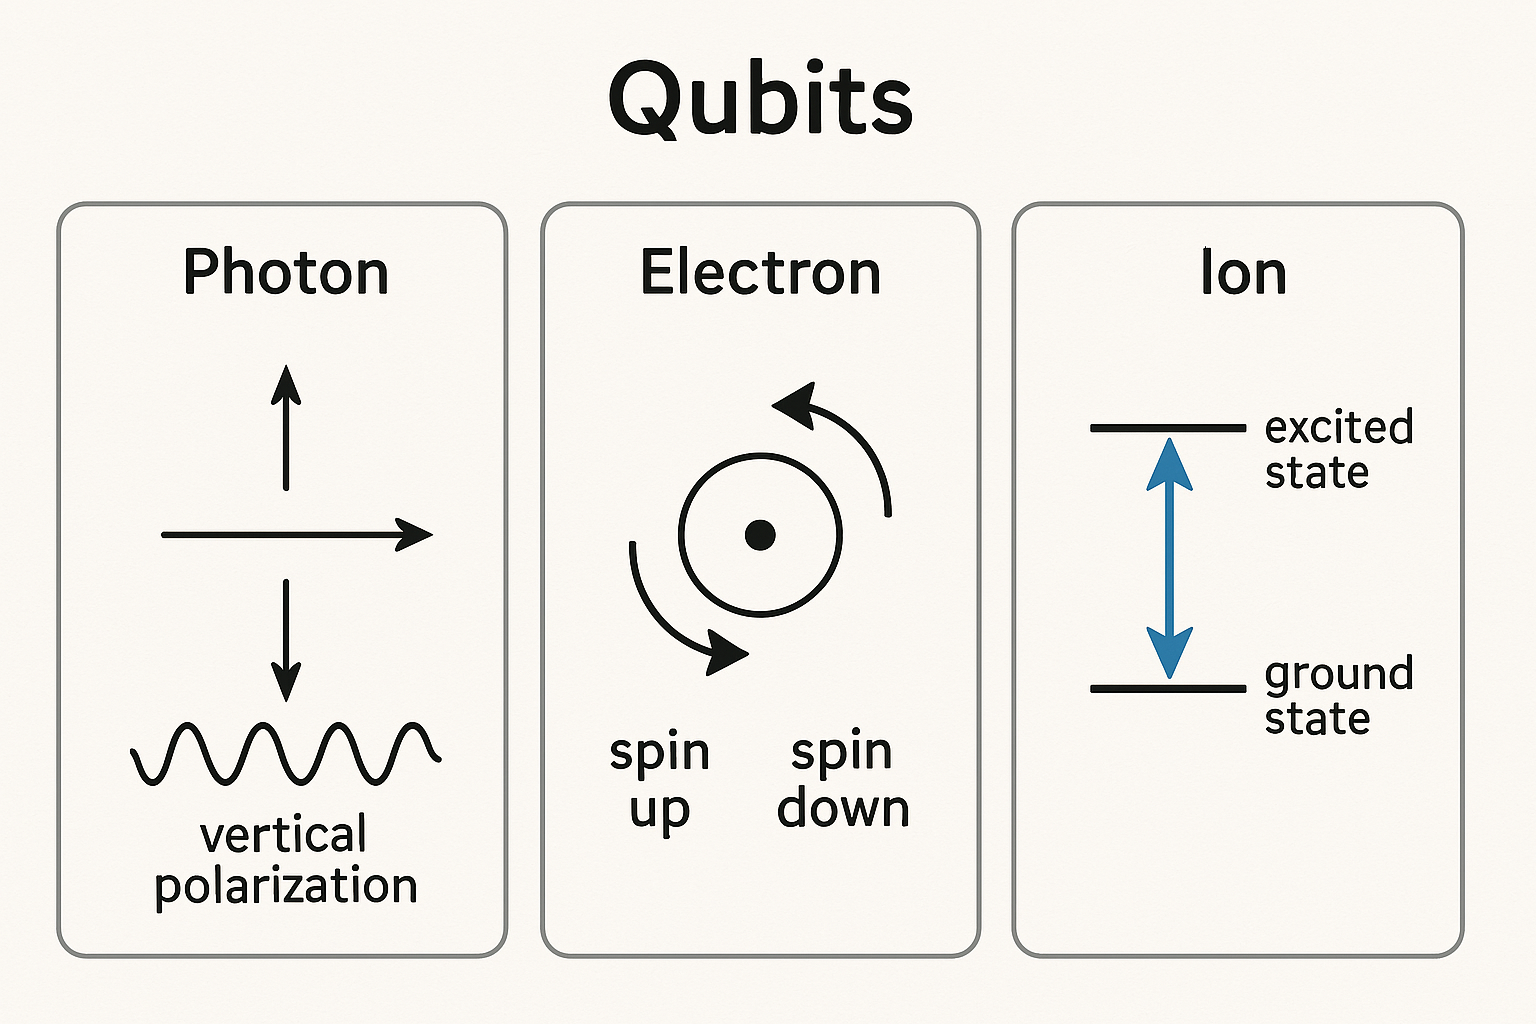
\includegraphics{figures/physical_qubits.png}
\caption{Physical Qubits}
\end{figure}

\begin{quote}
\textbf{Take-away:} physical implementation-ion-trap, superconducting,
photonic-can be abstracted as a \textbf{two-level quantum system} whose
logical states we call\\
\[
\lvert0\rangle,\; \lvert1\rangle .
\]
\end{quote}

\begin{itemize}
\tightlist
\item
  qubit is an analogous to classical bit;
\end{itemize}

\begin{longtable}[]{@{}
  >{\raggedright\arraybackslash}p{(\columnwidth - 2\tabcolsep) * \real{0.4000}}
  >{\raggedright\arraybackslash}p{(\columnwidth - 2\tabcolsep) * \real{0.6000}}@{}}
\toprule\noalign{}
\begin{minipage}[b]{\linewidth}\raggedright
Classical bit
\end{minipage} & \begin{minipage}[b]{\linewidth}\raggedright
Quantum bit (qubit)
\end{minipage} \\
\midrule\noalign{}
\endhead
\bottomrule\noalign{}
\endlastfoot
stores 0 \emph{or}~1 & stores a \textbf{state-vector} in
\(\mathbb C^{2}\) :
\(\displaystyle \lvert\psi\rangle=\alpha\lvert0\rangle+\beta\lvert1\rangle\) \\
operations are Boolean gates & operations are \textbf{unitaries}
(reversible 2×2 matrices) \\
\end{longtable}

\begin{center}\rule{0.5\linewidth}{0.5pt}\end{center}

\hypertarget{single-qubit-pure-state}{%
\subsubsection*{Single-qubit pure state}\label{single-qubit-pure-state}}

Quantum systems have states, and for a qubit those orthogonal states are
\( \lvert0\rangle\) and \(\lvert1\rangle \) {[}using ket notation{]}.

\begin{itemize}
\item
  \(\lvert0\rangle\) and \(\lvert1\rangle\) are known as the
  \emph{computational basis} states.
\item
  It is possible to have linear combinations of states, called
  \emph{superpositions} where \(\alpha\) \& \(\beta\) are complex
  values:

  \[|\psi\rangle = \alpha \lvert0\rangle + \beta \lvert1\rangle\]
\item
  \(\lvert0\rangle\) and \(\lvert1\rangle\) form an ortho-normal basis
  for the qubit 2-dimensional complex vector space.
\end{itemize}

\begin{center}\rule{0.5\linewidth}{0.5pt}\end{center}

\hypertarget{measurement-probabilities}{%
\subsubsection*{Measurement
Probabilities}\label{measurement-probabilities}}

\(\alpha\) \& \(\beta\) are (complex valued) amplitudes which give the
measurement probability on obtaining a basis outcome \(\lvert0\rangle\)
or \(\lvert1\rangle\).

\begin{itemize}
\item
  \(P(\lvert0\rangle) = \lvert\alpha\lvert^2 \quad P(\lvert1\rangle) = \lvert\beta\lvert^2\)
  \textgreater{} For a pure state of a 3 qubit register, the probability
  of measuring one basis state would be: \textgreater{} \textgreater{}
   \( P(\lvert010\rangle) = \lvert\alpha\_1\beta\_2\alpha\_3\lvert\^{}2 \)
\item
  The sum of probabilities of each of the basis outcomes must be 1,
  making the state a unit vector.
\item
  The quantum system is \emph{completely described} by this unit vector
  in the state space, its state-vector.

  \begin{quote}
  So the pure state \(\lvert\psi\rangle\) of a qubit is a unit vector in
  a 2-D complex vector space (actually \emph{Hilbert} space, we see
  later).

  \( \textbar{}\alpha\textbar\^{}2 + \textbar{}\beta\textbar\^{}2 =
  1 \rightarrow \) the state-vector is \textbf{unit-norm}.
  \end{quote}
\end{itemize}

\begin{center}\rule{0.5\linewidth}{0.5pt}\end{center}

\hypertarget{bloch-sphere-picture}{%
\subsubsection*{Bloch-sphere picture}\label{bloch-sphere-picture}}

All single-qubit pure states live on the unit sphere in
\(\mathbb C^{3}\):

\[
\lvert\psi\rangle
=\cos\frac{\theta}{2}\,\lvert0\rangle
+\;e^{i\varphi}\sin\frac{\theta}{2}\,\lvert1\rangle ,
\quad
0\le\theta\le\pi,\;0\le\varphi<2\pi .
\]

\begin{figure}
\centering
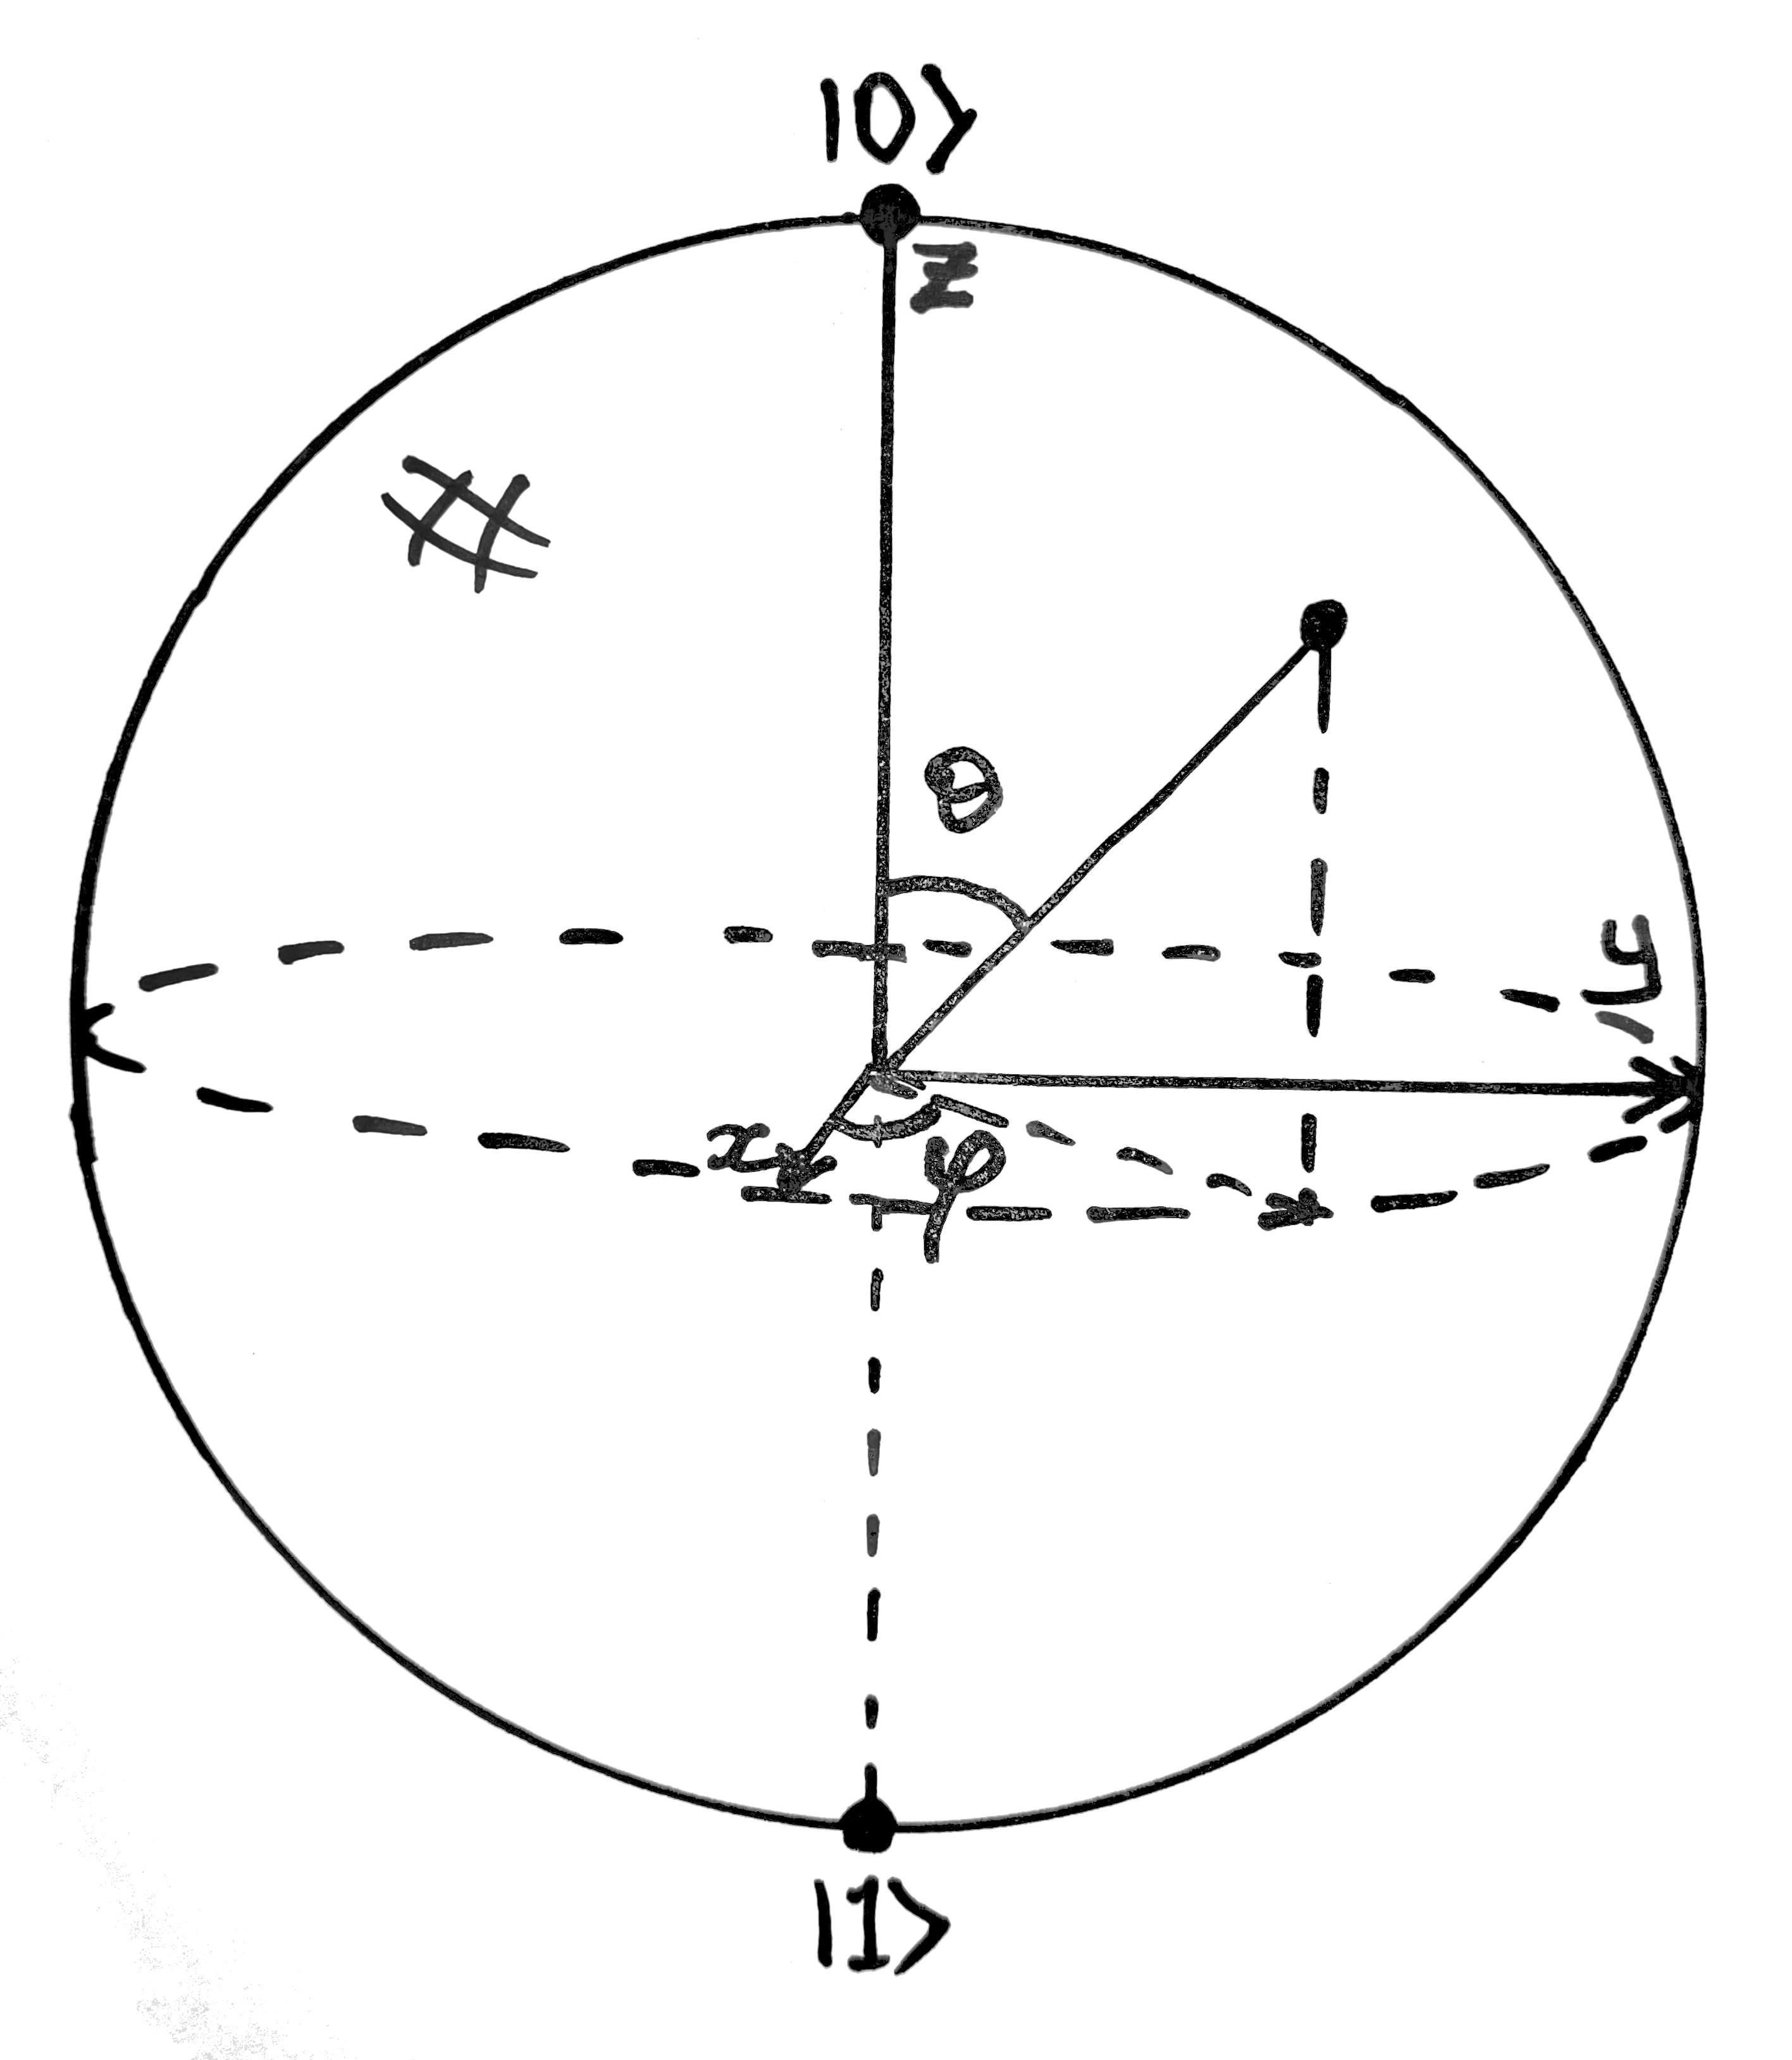
\includegraphics{figures/blochsphere.png}
\caption{Bloch sphere annotated}
\end{figure}

\begin{quote}
\emph{create a Bloch vector for \(\theta=\pi/3,\;\phi=\pi/2\) and plot
it.}
\end{quote}

    \begin{tcolorbox}[breakable, size=fbox, boxrule=1pt, pad at break*=1mm,colback=cellbackground, colframe=cellborder]
\prompt{In}{incolor}{1}{\boxspacing}
\begin{Verbatim}[commandchars=\\\{\}]
\PY{k+kn}{import} \PY{n+nn}{numpy} \PY{k}{as} \PY{n+nn}{np}
\PY{k+kn}{from} \PY{n+nn}{qiskit}\PY{n+nn}{.}\PY{n+nn}{visualization} \PY{k+kn}{import} \PY{n}{plot\PYZus{}bloch\PYZus{}vector}

\PY{n}{theta}\PY{p}{,} \PY{n}{phi} \PY{o}{=} \PY{n}{np}\PY{o}{.}\PY{n}{pi}\PY{o}{/}\PY{l+m+mi}{3}\PY{p}{,} \PY{n}{np}\PY{o}{.}\PY{n}{pi}\PY{o}{/}\PY{l+m+mi}{2}
\PY{n}{bloch\PYZus{}vec} \PY{o}{=} \PY{p}{[}\PY{n}{np}\PY{o}{.}\PY{n}{sin}\PY{p}{(}\PY{n}{theta}\PY{p}{)}\PY{o}{*}\PY{n}{np}\PY{o}{.}\PY{n}{cos}\PY{p}{(}\PY{n}{phi}\PY{p}{)}\PY{p}{,}   \PY{c+c1}{\PYZsh{} x}
             \PY{n}{np}\PY{o}{.}\PY{n}{sin}\PY{p}{(}\PY{n}{theta}\PY{p}{)}\PY{o}{*}\PY{n}{np}\PY{o}{.}\PY{n}{sin}\PY{p}{(}\PY{n}{phi}\PY{p}{)}\PY{p}{,}   \PY{c+c1}{\PYZsh{} y}
             \PY{n}{np}\PY{o}{.}\PY{n}{cos}\PY{p}{(}\PY{n}{theta}\PY{p}{)}\PY{p}{]}               \PY{c+c1}{\PYZsh{} z}
\PY{n}{plot\PYZus{}bloch\PYZus{}vector}\PY{p}{(}\PY{n}{bloch\PYZus{}vec}\PY{p}{)}
\end{Verbatim}
\end{tcolorbox}
 
            
\prompt{Out}{outcolor}{1}{}
    
    \begin{center}
    \adjustimage{max size={0.9\linewidth}{0.9\paperheight}}{figures/unit_2.0_from-qubits-to-linear-algebra_1_0.png}
    \end{center}
    { \hspace*{\fill} \\}
    

    \hypertarget{dirac-notation-multiqubit-basis}{%
\subsection*{2.1\,Dirac Notation \& Multi‑Qubit
Basis}\label{dirac-notation-multiqubit-basis}}

Compact bra‑ket language and the \(2^{n}\)-dimensional computational
basis for \(n\) qubits.

Provides the shorthand used in all quantum‑algorithm papers and allows
us to label, index and program multi‑qubit circuits unambiguously.

\begin{longtable}[]{@{}
  >{\raggedright\arraybackslash}p{(\columnwidth - 2\tabcolsep) * \real{0.4000}}
  >{\raggedright\arraybackslash}p{(\columnwidth - 2\tabcolsep) * \real{0.6000}}@{}}
\toprule\noalign{}
\begin{minipage}[b]{\linewidth}\raggedright
Code
\end{minipage} & \begin{minipage}[b]{\linewidth}\raggedright
Outcome
\end{minipage} \\
\midrule\noalign{}
\endhead
\bottomrule\noalign{}
\endlastfoot
\,2.1‑A & \textbf{translate} between column‑vector and
\(\lvert\cdot\rangle\) notation for any 2‑component state. \\
\,2.1‑B & \textbf{enumerate} all \(2^{n}\) computational basis states
for \(n\le 3\) and \textbf{state} the dimension of the Hilbert space. \\
\,2.1‑C & \textbf{normalise} a given two‑qubit amplitude list and
\textbf{verify} the norm with Python. \\
\end{longtable}

\begin{center}\rule{0.5\linewidth}{0.5pt}\end{center}

\hypertarget{kets-and-bras}{%
\paragraph{Kets and Bras}\label{kets-and-bras}}

A \textbf{ket} is a column vector

\[
\lvert\psi\rangle \;=\;
\begin{pmatrix}
\psi_0 \\ \psi_1 \\ \vdots \\ \psi_{d-1}
\end{pmatrix},
\] while its \textbf{bra} is the conjugate‑transpose (row)\\
\[
\langle\psi\lvert \;=\;
\bigl(\psi_0^{\!*},\;\psi_1^{\!*},\;\dots,\;\psi_{d-1}^{\!*}\bigr).
\]

\begin{center}\rule{0.5\linewidth}{0.5pt}\end{center}

\hypertarget{computational-basis}{%
\paragraph{Computational basis}\label{computational-basis}}

Dirac notation uses bit strings \(\{0,1\}^n\) (e.g.~\(\lvert0\rangle\)
and \(\lvert1\rangle\))

\begin{itemize}
\tightlist
\item
  For \(n\) qubits the \emph{computational (standard) basis} is\\
  \textgreater{}
  \(\bigl\{\;\lvert x\rangle : x\in\{0,1\}^{\,n}\bigr\},\)
  \textgreater{} \textgreater{} a set of \(2^{n}\) mutually orthonormal
  vectors. \textgreater{} \textgreater{} If \(n = 3\), one standard
  basis is \(\lvert011\rangle\), and \(\langle011\lvert\) is the row
  vector: \((00010000)\).
\end{itemize}

\begin{center}\rule{0.5\linewidth}{0.5pt}\end{center}

\hypertarget{example---two-qubits}{%
\paragraph{Example - two qubits}\label{example---two-qubits}}

A general pure state of two qubits is

\[
\lvert\phi\rangle \;=\;
\alpha_{00}\lvert 00\rangle + 
\alpha_{01}\lvert 01\rangle + 
\alpha_{10}\lvert 10\rangle + 
\alpha_{11}\lvert 11\rangle
\] \[
\qquad
\|\phi\|^{2}
=\sum_{i,j\in\{0,1\}} |\alpha_{ij}|^{2}=1 .
\]

    \begin{tcolorbox}[breakable, size=fbox, boxrule=1pt, pad at break*=1mm,colback=cellbackground, colframe=cellborder]
\prompt{In}{incolor}{2}{\boxspacing}
\begin{Verbatim}[commandchars=\\\{\}]
\PY{c+c1}{\PYZsh{}\PYZsh{}\PYZsh{}\PYZsh{} Quick Python check \PYZhy{} normalise a random two\PYZhy{}qubit state}
\PY{k+kn}{import} \PY{n+nn}{numpy} \PY{k}{as} \PY{n+nn}{np}

\PY{c+c1}{\PYZsh{} random complex amplitudes}
\PY{n}{amps} \PY{o}{=} \PY{n}{np}\PY{o}{.}\PY{n}{random}\PY{o}{.}\PY{n}{randn}\PY{p}{(}\PY{l+m+mi}{4}\PY{p}{)} \PY{o}{+} \PY{l+m+mi}{1}\PY{n}{j}\PY{o}{*}\PY{n}{np}\PY{o}{.}\PY{n}{random}\PY{o}{.}\PY{n}{randn}\PY{p}{(}\PY{l+m+mi}{4}\PY{p}{)}
\PY{n}{phi}  \PY{o}{=} \PY{n}{amps} \PY{o}{/} \PY{n}{np}\PY{o}{.}\PY{n}{linalg}\PY{o}{.}\PY{n}{norm}\PY{p}{(}\PY{n}{amps}\PY{p}{)}          \PY{c+c1}{\PYZsh{} normalise}

\PY{n+nb}{print}\PY{p}{(}\PY{l+s+s2}{\PYZdq{}}\PY{l+s+s2}{State vector |φ⟩ =}\PY{l+s+s2}{\PYZdq{}}\PY{p}{,} \PY{n}{phi}\PY{p}{)}
\PY{n+nb}{print}\PY{p}{(}\PY{l+s+s2}{\PYZdq{}}\PY{l+s+s2}{Norm² =}\PY{l+s+s2}{\PYZdq{}}\PY{p}{,} \PY{n}{np}\PY{o}{.}\PY{n}{vdot}\PY{p}{(}\PY{n}{phi}\PY{p}{,} \PY{n}{phi}\PY{p}{)}\PY{o}{.}\PY{n}{real}\PY{p}{)}    \PY{c+c1}{\PYZsh{} should print 1.0}
\end{Verbatim}
\end{tcolorbox}

    \begin{Verbatim}[commandchars=\\\{\}]
State vector |φ⟩ = [-0.73202702-0.03449025j -0.20235518+0.3679845j
0.10864371-0.09399594j
  0.49096349-0.15780625j]
Norm² = 1.0
    \end{Verbatim}

    \hypertarget{vector-spaces-refresher}{%
\subsection*{2.2\,Vector Spaces
Refresher}\label{vector-spaces-refresher}}

Addition, scalar multiplication, spanning sets, linear independence, and
what a \emph{basis} really is.

These are the axioms under every quantum proof; without them you can't
talk about dimensions, change‑of‑basis, or well‑posed linear systems.

\begin{longtable}[]{@{}
  >{\raggedright\arraybackslash}p{(\columnwidth - 2\tabcolsep) * \real{0.4000}}
  >{\raggedright\arraybackslash}p{(\columnwidth - 2\tabcolsep) * \real{0.6000}}@{}}
\toprule\noalign{}
\begin{minipage}[b]{\linewidth}\raggedright
Code
\end{minipage} & \begin{minipage}[b]{\linewidth}\raggedright
Outcome
\end{minipage} \\
\midrule\noalign{}
\endhead
\bottomrule\noalign{}
\endlastfoot
\,2.2‑A & \textbf{perform} vector addition and scalar multiplication on
complex \(n\)-tuples in code. \\
\,2.2‑B & \textbf{identify} whether a provided set of vectors in
\(\mathbb C^{n}\) is linearly independent. \\
\,2.2‑C & \textbf{express} \(\lvert0\rangle,\lvert1\rangle\) as explicit
column matrices and \textbf{show} they form a basis of
\(\mathbb C^{2}\). \\
\end{longtable}

\begin{center}\rule{0.5\linewidth}{0.5pt}\end{center}

\hypertarget{complex-vector-space-addition-and-scalar-multiplication}{%
\paragraph{Complex Vector Space Addition and Scalar
multiplication}\label{complex-vector-space-addition-and-scalar-multiplication}}

A complex vector space \textbf{vector space} V over \(\mathbb C\) of
dimension \(n\), \(V=C^n\), is the set\\
\[
\mathbb C^{\,n}\;=\;\bigl\{(z_{1},\dots,z_{n})^{T}\;|\;z_k\in\mathbb C\bigr\},
\] equipped with

\begin{itemize}
\item
  \textbf{Addition}\\
  \[
  (v+w)_k \;=\; v_k + w_k ,
  \]
\item
  \textbf{Scalar multiplication}\\
  \[
  (\lambda v)_k \;=\; \lambda\,v_k ,\quad \lambda\in\mathbb C .
  \]
\end{itemize}

The \textbf{zero vector} \(0=(0,\dots,0)^{T}\) satisfies \(v+0=v\).

\begin{itemize}
\item
  \textbf{Zero vector} \(0\) has all elements as 0: \((0, 0, ... , 0)\)
\item
  \textbf{Zero element}
\end{itemize}

\begin{center}\rule{0.5\linewidth}{0.5pt}\end{center}

\hypertarget{spanning-sets-bases}{%
\paragraph{Spanning Sets \& Bases}\label{spanning-sets-bases}}

A list of vectors \(\{v_1,\dots,v_m\}\subseteq\mathbb C^{n}\)

\begin{itemize}
\tightlist
\item
  \textbf{spans} the space if every \(u\in\mathbb C^{n}\) can be
  written\\
  \(u=\sum_{j=1}^{m} \alpha_j v_j\).\\
\item
  is \textbf{linearly independent} if \(\sum\alpha_j v_j = 0\) implies
  all \(\alpha_j=0\).
\end{itemize}

If it both spans and is independent, it is a \textbf{basis}; any basis
of \(\mathbb C^{n}\) contains exactly \(n\) vectors.

\begin{center}\rule{0.5\linewidth}{0.5pt}\end{center}

\hypertarget{singlequbit-example}{%
\paragraph{Single‑Qubit Example}\label{singlequbit-example}}

For one qubit, the matrix representation the computational--basis kets,
\(\lvert0\rangle\) and \(\lvert1\rangle\), are: \[
\lvert0\rangle=\begin{pmatrix}1\\0\end{pmatrix},
\quad
\lvert1\rangle=\begin{pmatrix}0\\1\end{pmatrix}
\]

\begin{itemize}
\item
  They span \(\mathbb C^{2}\)
\item
  Are independent because neither row elements sum to zero:
  \(1 + 0 = 1\) and \(0 + 1 = 1\)
\item
  Therefore form a basis.
\end{itemize}

\begin{center}\rule{0.5\linewidth}{0.5pt}\end{center}

    \begin{tcolorbox}[breakable, size=fbox, boxrule=1pt, pad at break*=1mm,colback=cellbackground, colframe=cellborder]
\prompt{In}{incolor}{3}{\boxspacing}
\begin{Verbatim}[commandchars=\\\{\}]
\PY{c+c1}{\PYZsh{}\PYZsh{}\PYZsh{}\PYZsh{} Python demo \PYZhy{} linear independence test}
\PY{k+kn}{import} \PY{n+nn}{numpy} \PY{k}{as} \PY{n+nn}{np}

\PY{n}{e0} \PY{o}{=} \PY{n}{np}\PY{o}{.}\PY{n}{array}\PY{p}{(}\PY{p}{[}\PY{l+m+mi}{1}\PY{p}{,}\PY{l+m+mi}{0}\PY{p}{]}\PY{p}{)}
\PY{n}{e1} \PY{o}{=} \PY{n}{np}\PY{o}{.}\PY{n}{array}\PY{p}{(}\PY{p}{[}\PY{l+m+mi}{0}\PY{p}{,}\PY{l+m+mi}{1}\PY{p}{]}\PY{p}{)}
\PY{n}{M}  \PY{o}{=} \PY{n}{np}\PY{o}{.}\PY{n}{column\PYZus{}stack}\PY{p}{(}\PY{p}{[}\PY{n}{e0}\PY{p}{,} \PY{n}{e1}\PY{p}{]}\PY{p}{)}   \PY{c+c1}{\PYZsh{} 2×2 matrix whose columns are the vectors}

\PY{n}{rank} \PY{o}{=} \PY{n}{np}\PY{o}{.}\PY{n}{linalg}\PY{o}{.}\PY{n}{matrix\PYZus{}rank}\PY{p}{(}\PY{n}{M}\PY{p}{)}
\PY{n+nb}{print}\PY{p}{(}\PY{l+s+s2}{\PYZdq{}}\PY{l+s+s2}{Rank =}\PY{l+s+s2}{\PYZdq{}}\PY{p}{,} \PY{n}{rank}\PY{p}{,} \PY{l+s+s2}{\PYZdq{}}\PY{l+s+s2}{ (basis)}\PY{l+s+s2}{\PYZdq{}} \PY{k}{if} \PY{n}{rank}\PY{o}{==}\PY{l+m+mi}{2} \PY{k}{else} \PY{l+s+s2}{\PYZdq{}}\PY{l+s+s2}{ (not independent)}\PY{l+s+s2}{\PYZdq{}}\PY{p}{)}

\PY{c+c1}{\PYZsh{} Verify in Python that X ∣0⟩=∣1⟩X∣0⟩=∣1⟩.}
\PY{n}{X} \PY{o}{=} \PY{n}{np}\PY{o}{.}\PY{n}{array}\PY{p}{(}\PY{p}{[}\PY{p}{[}\PY{l+m+mi}{0}\PY{p}{,}\PY{l+m+mi}{1}\PY{p}{]}\PY{p}{,}\PY{p}{[}\PY{l+m+mi}{1}\PY{p}{,}\PY{l+m+mi}{0}\PY{p}{]}\PY{p}{]}\PY{p}{)}
\PY{n+nb}{print}\PY{p}{(}\PY{l+s+s2}{\PYZdq{}}\PY{l+s+s2}{X}\PY{l+s+s2}{\PYZbs{}}\PY{l+s+s2}{lvert0}\PY{l+s+se}{\PYZbs{}r}\PY{l+s+s2}{angle =}\PY{l+s+s2}{\PYZdq{}}\PY{p}{,} \PY{n}{X}\PY{o}{.}\PY{n}{dot}\PY{p}{(}\PY{n}{e0}\PY{p}{)}\PY{p}{)}
\end{Verbatim}
\end{tcolorbox}

    \begin{Verbatim}[commandchars=\\\{\}]
Rank = 2  (basis)
angle = [0 1]
    \end{Verbatim}

    \hypertarget{linear-operators-pauli-friends}{%
\subsection*{2.3\,Linear Operators (Pauli \&
Friends)}\label{linear-operators-pauli-friends}}

Definition of a linear operator, identity/zero maps, and the Pauli
matrices as elementary single‑qubit unitaries.

Gates \emph{are} linear operators; mastering Pauli algebra is
prerequisite for circuit decomposition, error correction and Hamiltonian
simulation.

\begin{longtable}[]{@{}
  >{\raggedright\arraybackslash}p{(\columnwidth - 2\tabcolsep) * \real{0.4000}}
  >{\raggedright\arraybackslash}p{(\columnwidth - 2\tabcolsep) * \real{0.6000}}@{}}
\toprule\noalign{}
\begin{minipage}[b]{\linewidth}\raggedright
Code
\end{minipage} & \begin{minipage}[b]{\linewidth}\raggedright
Outcome
\end{minipage} \\
\midrule\noalign{}
\endhead
\bottomrule\noalign{}
\endlastfoot
\,2.3‑A & \textbf{verify} line‑arity of a given matrix function \(A(v)\)
by symbolic or numeric test. \\
\,2.3‑B & \textbf{construct} the Pauli matrices in NumPy and
\textbf{demonstrate} \(X^{2}=Y^{2}=Z^{2}=I\). \\
\,2.3‑C & \textbf{explain} in ≤\,3 sentences why single‑qubit gates must
be unitary (linking to reversibility). \\
\end{longtable}

\begin{center}\rule{0.5\linewidth}{0.5pt}\end{center}

\hypertarget{what-is-a-linear-operator}{%
\paragraph{What is a Linear Operator?}\label{what-is-a-linear-operator}}

\begin{itemize}
\tightlist
\item
  linear operator as a function mapping vector spaces V -\textgreater{}
  W;
\end{itemize}

A map \(A : V \rightarrow V\) on a vector space \(V\) is \textbf{linear}
if\\
\[
A\bigl(\lambda v + w\bigr) \;=\; \lambda\,A v + A w
\qquad\forall\, v,w\in V,\;\lambda\in\mathbb C .
\]

\begin{itemize}
\item
  \textbf{Identity operator} \(I\) satisfies \(I v = v\).
\item
  Identity matrix:
\item
  \textbf{Zero operator} \(0\) maps a vector to zero vector and
  satisfies \(0 v = 0\).
\end{itemize}

\begin{center}\rule{0.5\linewidth}{0.5pt}\end{center}

\hypertarget{singlequbit-pauli-set}{%
\paragraph{Single‑Qubit Pauli Set}\label{singlequbit-pauli-set}}

\[
I \;=\;
\begin{pmatrix}
1 & 0 \\
0 & 1
\end{pmatrix},
\quad
X \;=\;
\begin{pmatrix}
0 & 1 \\
1 & 0
\end{pmatrix},
\quad
Y \;=\;
\begin{pmatrix}
0 & -i \\
i & 0
\end{pmatrix},
\quad
Z \;=\;
\begin{pmatrix}
1 & 0 \\
0 & -1
\end{pmatrix}.
\]

\begin{itemize}
\tightlist
\item
  \textbf{Hermitian}: \(P^\dagger = P\).\\
\item
  \textbf{Unitary}: \(P^\dagger P = I\).\\
\item
  \textbf{Squares to identity}: \(P^{2}=I\).
\end{itemize}

These four matrices plus overall phases generate all single‑qubit
unitaries.

\begin{center}\rule{0.5\linewidth}{0.5pt}\end{center}

\hypertarget{action-on-the-bloch-sphere}{%
\paragraph{Action on the Bloch
Sphere}\label{action-on-the-bloch-sphere}}

\begin{itemize}
\tightlist
\item
  \(X\)\,--- rotation by \(\pi\) around the \textbf{x‑axis}\\
\item
  \(Y\)\,--- rotation by \(\pi\) around the \textbf{y‑axis}\\
\item
  \(Z\)\,--- rotation by \(\pi\) around the \textbf{z‑axis}
\end{itemize}

\begin{figure}
\centering
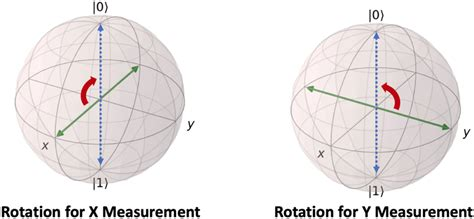
\includegraphics{figures/pauli_axes.jpeg}
\caption{Pauli rotations}
\end{figure}

\begin{center}\rule{0.5\linewidth}{0.5pt}\end{center}

    \begin{tcolorbox}[breakable, size=fbox, boxrule=1pt, pad at break*=1mm,colback=cellbackground, colframe=cellborder]
\prompt{In}{incolor}{4}{\boxspacing}
\begin{Verbatim}[commandchars=\\\{\}]
\PY{c+c1}{\PYZsh{}\PYZsh{}\PYZsh{}\PYZsh{} Python sandbox \PYZhy{} verify Pauli algebra}
\PY{k+kn}{import} \PY{n+nn}{numpy} \PY{k}{as} \PY{n+nn}{np}

\PY{n}{I} \PY{o}{=} \PY{n}{np}\PY{o}{.}\PY{n}{eye}\PY{p}{(}\PY{l+m+mi}{2}\PY{p}{,} \PY{n}{dtype}\PY{o}{=}\PY{n+nb}{complex}\PY{p}{)}
\PY{n}{X} \PY{o}{=} \PY{n}{np}\PY{o}{.}\PY{n}{array}\PY{p}{(}\PY{p}{[}\PY{p}{[}\PY{l+m+mi}{0}\PY{p}{,}\PY{l+m+mi}{1}\PY{p}{]}\PY{p}{,}\PY{p}{[}\PY{l+m+mi}{1}\PY{p}{,}\PY{l+m+mi}{0}\PY{p}{]}\PY{p}{]}\PY{p}{,} \PY{n}{dtype}\PY{o}{=}\PY{n+nb}{complex}\PY{p}{)}
\PY{n}{Y} \PY{o}{=} \PY{n}{np}\PY{o}{.}\PY{n}{array}\PY{p}{(}\PY{p}{[}\PY{p}{[}\PY{l+m+mi}{0}\PY{p}{,}\PY{o}{\PYZhy{}}\PY{l+m+mi}{1}\PY{n}{j}\PY{p}{]}\PY{p}{,}\PY{p}{[}\PY{l+m+mi}{1}\PY{n}{j}\PY{p}{,}\PY{l+m+mi}{0}\PY{p}{]}\PY{p}{]}\PY{p}{,} \PY{n}{dtype}\PY{o}{=}\PY{n+nb}{complex}\PY{p}{)}
\PY{n}{Z} \PY{o}{=} \PY{n}{np}\PY{o}{.}\PY{n}{array}\PY{p}{(}\PY{p}{[}\PY{p}{[}\PY{l+m+mi}{1}\PY{p}{,}\PY{l+m+mi}{0}\PY{p}{]}\PY{p}{,}\PY{p}{[}\PY{l+m+mi}{0}\PY{p}{,}\PY{o}{\PYZhy{}}\PY{l+m+mi}{1}\PY{p}{]}\PY{p}{]}\PY{p}{,} \PY{n}{dtype}\PY{o}{=}\PY{n+nb}{complex}\PY{p}{)}

\PY{k}{for} \PY{n}{name}\PY{p}{,} \PY{n}{P} \PY{o+ow}{in} \PY{p}{[}\PY{p}{(}\PY{l+s+s1}{\PYZsq{}}\PY{l+s+s1}{X}\PY{l+s+s1}{\PYZsq{}}\PY{p}{,}\PY{n}{X}\PY{p}{)}\PY{p}{,} \PY{p}{(}\PY{l+s+s1}{\PYZsq{}}\PY{l+s+s1}{Y}\PY{l+s+s1}{\PYZsq{}}\PY{p}{,}\PY{n}{Y}\PY{p}{)}\PY{p}{,} \PY{p}{(}\PY{l+s+s1}{\PYZsq{}}\PY{l+s+s1}{Z}\PY{l+s+s1}{\PYZsq{}}\PY{p}{,}\PY{n}{Z}\PY{p}{)}\PY{p}{]}\PY{p}{:}
    \PY{n+nb}{print}\PY{p}{(}\PY{l+s+sa}{f}\PY{l+s+s2}{\PYZdq{}}\PY{l+s+si}{\PYZob{}}\PY{n}{name}\PY{l+s+si}{\PYZcb{}}\PY{l+s+s2}{² == I ?}\PY{l+s+s2}{\PYZdq{}}\PY{p}{,} \PY{n}{np}\PY{o}{.}\PY{n}{allclose}\PY{p}{(}\PY{n}{P} \PY{o}{@} \PY{n}{P}\PY{p}{,} \PY{n}{I}\PY{p}{)}\PY{p}{)}
    \PY{n+nb}{print}\PY{p}{(}\PY{l+s+sa}{f}\PY{l+s+s2}{\PYZdq{}}\PY{l+s+si}{\PYZob{}}\PY{n}{name}\PY{l+s+si}{\PYZcb{}}\PY{l+s+s2}{† }\PY{l+s+si}{\PYZob{}}\PY{n}{name}\PY{l+s+si}{\PYZcb{}}\PY{l+s+s2}{ == I ?}\PY{l+s+s2}{\PYZdq{}}\PY{p}{,} \PY{n}{np}\PY{o}{.}\PY{n}{allclose}\PY{p}{(}\PY{n}{P}\PY{o}{.}\PY{n}{conj}\PY{p}{(}\PY{p}{)}\PY{o}{.}\PY{n}{T} \PY{o}{@} \PY{n}{P}\PY{p}{,} \PY{n}{I}\PY{p}{)}\PY{p}{)}

\PY{k+kn}{import} \PY{n+nn}{numpy} \PY{k}{as} \PY{n+nn}{np}
\PY{n}{I} \PY{o}{=} \PY{n}{np}\PY{o}{.}\PY{n}{eye}\PY{p}{(}\PY{l+m+mi}{2}\PY{p}{)}
\PY{n}{X} \PY{o}{=} \PY{n}{np}\PY{o}{.}\PY{n}{array}\PY{p}{(}\PY{p}{[}\PY{p}{[}\PY{l+m+mi}{0}\PY{p}{,}\PY{l+m+mi}{1}\PY{p}{]}\PY{p}{,}\PY{p}{[}\PY{l+m+mi}{1}\PY{p}{,}\PY{l+m+mi}{0}\PY{p}{]}\PY{p}{]}\PY{p}{)}
\PY{n}{Y} \PY{o}{=} \PY{n}{np}\PY{o}{.}\PY{n}{array}\PY{p}{(}\PY{p}{[}\PY{p}{[}\PY{l+m+mi}{0}\PY{p}{,}\PY{o}{\PYZhy{}}\PY{l+m+mi}{1}\PY{n}{j}\PY{p}{]}\PY{p}{,}\PY{p}{[}\PY{l+m+mi}{1}\PY{n}{j}\PY{p}{,}\PY{l+m+mi}{0}\PY{p}{]}\PY{p}{]}\PY{p}{)}
\PY{n}{Z} \PY{o}{=} \PY{n}{np}\PY{o}{.}\PY{n}{array}\PY{p}{(}\PY{p}{[}\PY{p}{[}\PY{l+m+mi}{1}\PY{p}{,}\PY{l+m+mi}{0}\PY{p}{]}\PY{p}{,}\PY{p}{[}\PY{l+m+mi}{0}\PY{p}{,}\PY{o}{\PYZhy{}}\PY{l+m+mi}{1}\PY{p}{]}\PY{p}{]}\PY{p}{)}
\end{Verbatim}
\end{tcolorbox}

    \begin{Verbatim}[commandchars=\\\{\}]
X² == I ? True
X† X == I ? True
Y² == I ? True
Y† Y == I ? True
Z² == I ? True
Z† Z == I ? True
    \end{Verbatim}

    Exercise: verify \(X^2=Y^2=Z^2=IX^2=Y^2=Z^2=I\).

\begin{verbatim}
Bloch‑sphere view — XX flips the sphere around the x‑axis, ZZ around z‑axis (see textbook figures pauli_x.png, pauli_z.png).
\end{verbatim}

    \hypertarget{inner-product-norm-orthogonality}{%
\subsection*{2.4\,Inner Product, Norm \&
Orthogonality}\label{inner-product-norm-orthogonality}}

The Dirac inner product, state normalisation and the geometric test for
orthogonality.

Inner products become measurement probabilities and kernel entries;
norms guarantee those probabilities sum to\,1 and ensure numerical
stability.

\begin{longtable}[]{@{}
  >{\raggedright\arraybackslash}p{(\columnwidth - 2\tabcolsep) * \real{0.4000}}
  >{\raggedright\arraybackslash}p{(\columnwidth - 2\tabcolsep) * \real{0.6000}}@{}}
\toprule\noalign{}
\begin{minipage}[b]{\linewidth}\raggedright
Code
\end{minipage} & \begin{minipage}[b]{\linewidth}\raggedright
Outcome
\end{minipage} \\
\midrule\noalign{}
\endhead
\bottomrule\noalign{}
\endlastfoot
\,2.4‑A & \textbf{compute} \(\langle v \lvert w\rangle\) for two
arbitrary complex vectors with a helper function. \\
\,2.4‑B & \textbf{determine} if two qubit states are orthogonal via the
inner product. \\
\,2.4‑C & \textbf{normalise} any non‑zero state vector to unit norm
using Python. \\
\end{longtable}

\begin{center}\rule{0.5\linewidth}{0.5pt}\end{center}

\hypertarget{dual-vector-in-dirac-braket-notation}{%
\subsubsection*{Dual Vector in Dirac (Bra--Ket)
Notation}\label{dual-vector-in-dirac-braket-notation}}

Given a ket\\
\[
\boxed{\;\lvert\psi\rangle \in \mathcal H\;}
\]\\
--- a column vector in the Hilbert space \(\mathcal H\) ---

its \textbf{dual vector} (or \textbf{bra}) is

\[
\boxed{\;\langle\psi\rvert \equiv \bigl(\lvert\psi\rangle\bigr)^{\dagger}\;}
\]

\begin{itemize}
\item
  \textbf{Mathematically:}\\
  \(\langle\psi|\) lives in the \textbf{dual space} \(\mathcal H^{*}\),
  the set of linear functionals that map kets to complex numbers.
\item
  \textbf{Operationally:}\\
  For any ket \(\lvert\phi\rangle\), \[
  \langle\psi\,|\,\phi\rangle
  = \mathrm{inner\;product}(\psi,\phi)
  \in \mathbb C .
  \]
\item
  \textbf{Matrix picture:}\\
  If \(\lvert\psi\rangle\) is the column vector
  \(\begin{pmatrix}\psi_0\\\psi_1\\\vdots\end{pmatrix}\), then\\
  \[
  \langle\psi\rvert = \bigl(\psi_0^{\!*},\;\psi_1^{\!*},\;\dots\bigr)
  \] --- i.e., the \textbf{conjugate‑transpose} (adjoint) of the ket.
\end{itemize}

Thus the bra \(\langle\psi|\) is the dual vector that, via the inner
product, turns any ket into a complex scalar.

\begin{center}\rule{0.5\linewidth}{0.5pt}\end{center}

\hypertarget{matrix-refresher-adjoint-conjugatetranspose-of-a-complex-matrix}{%
\paragraph{Matrix refresher Adjoint (Conjugate‑Transpose) of a Complex
Matrix}\label{matrix-refresher-adjoint-conjugatetranspose-of-a-complex-matrix}}

\textbf{Complex Conjugate}

For any complex number \(z = a + ib , \qquad a,b\in\mathbb R\), its
\textbf{conjugate} is \(z^{*} = a - ib\).

That is:

\begin{longtable}[]{@{}lll@{}}
\toprule\noalign{}
Component & Before conjugation & After conjugation \\
\midrule\noalign{}
\endhead
\bottomrule\noalign{}
\endlastfoot
Real part &  \( \operatorname{Re}(z)=a  \) & \textbf{unchanged} \\
Imag part &  \( \operatorname{Im}(z)=b  \) & \textbf{sign flips} →
\(-b\) \\
\end{longtable}

\textbf{Adjoint (Conjugate‑Transpose)}

For any complex matrix \(A \in \mathbb{C}^{m\times n}\), the
\textbf{adjoint}---also called the \textbf{Hermitian conjugate} or
\textbf{conjugate‑transpose}---is denoted \(A^{\dagger}\) and defined by

\[
\boxed{\;
A^{\dagger} \;=\; \bigl(A^{*}\bigr)^{\mathsf T}
\;}
\]

where

\begin{itemize}
\tightlist
\item
  \(A^{*}\) = element‑wise \textbf{complex conjugate} of \(A\)\\
\item
  \((\cdot)^{\mathsf T}\) = \textbf{transpose} operation (rows ↔
  columns).
\end{itemize}

Equivalently, the matrix elements satisfy

\[
\bigl(A^{\dagger}\bigr)_{ij} = \bigl(A_{ji}\bigr)^{*}.
\]

\hypertarget{key-properties}{%
\subparagraph{Key properties}\label{key-properties}}

\begin{itemize}
\tightlist
\item
  \(\bigl(A^{\dagger}\bigr)^{\dagger} = A\)\\
\item
  \((AB)^{\dagger} = B^{\dagger}A^{\dagger}\) (order reverses)\\
\item
  A matrix is \textbf{Hermitian} if \(A^{\dagger}=A\); \textbf{unitary}
  if \(A^{\dagger}A = I\).
\end{itemize}

    \begin{tcolorbox}[breakable, size=fbox, boxrule=1pt, pad at break*=1mm,colback=cellbackground, colframe=cellborder]
\prompt{In}{incolor}{5}{\boxspacing}
\begin{Verbatim}[commandchars=\\\{\}]
\PY{k+kn}{import} \PY{n+nn}{numpy} \PY{k}{as} \PY{n+nn}{np}

\PY{n}{A} \PY{o}{=} \PY{n}{np}\PY{o}{.}\PY{n}{array}\PY{p}{(}\PY{p}{[}\PY{p}{[}\PY{l+m+mi}{1}\PY{o}{+}\PY{l+m+mi}{2}\PY{n}{j}\PY{p}{,} \PY{l+m+mi}{3}\PY{o}{\PYZhy{}}\PY{l+m+mi}{1}\PY{n}{j}\PY{p}{]}\PY{p}{,}
              \PY{p}{[}\PY{l+m+mi}{4}\PY{o}{+}\PY{l+m+mi}{0}\PY{n}{j}\PY{p}{,} \PY{l+m+mi}{5}\PY{o}{+}\PY{l+m+mi}{5}\PY{n}{j}\PY{p}{]}\PY{p}{]}\PY{p}{)}

\PY{n}{A\PYZus{}dag} \PY{o}{=} \PY{n}{A}\PY{o}{.}\PY{n}{conj}\PY{p}{(}\PY{p}{)}\PY{o}{.}\PY{n}{T}    \PY{c+c1}{\PYZsh{} conjugate\PYZhy{}transpose}
\PY{n+nb}{print}\PY{p}{(}\PY{l+s+s2}{\PYZdq{}}\PY{l+s+s2}{A† =}\PY{l+s+se}{\PYZbs{}n}\PY{l+s+s2}{\PYZdq{}}\PY{p}{,} \PY{n}{A\PYZus{}dag}\PY{p}{)}
\end{Verbatim}
\end{tcolorbox}

    \begin{Verbatim}[commandchars=\\\{\}]
A† =
 [[1.-2.j 4.-0.j]
 [3.+1.j 5.-5.j]]
    \end{Verbatim}

    \begin{center}\rule{0.5\linewidth}{0.5pt}\end{center}

\hypertarget{dirac-inner-product}{%
\paragraph{Dirac Inner Product}\label{dirac-inner-product}}

Notation if inner product of two states : \(\langle v | w \rangle\) or
\((v,w)\).

For vectors \(v,w\in\mathbb C^{\,n}\)

\[
\boxed{\;
\langle v \,|\, w\rangle \;=\; v^{\dagger} w
\;=\; \sum_{k=1}^{n} v_k^{\!*}\,w_k
\;}
\]

\begin{itemize}
\tightlist
\item
  \textbf{Conjugate
  symmetry} \(\langle v|w\rangle = \langle w|v\rangle^{*}\)\\
\item
  \textbf{Linearity in the second
  slot} \(\langle v|(\alpha w+\beta u)\rangle = \alpha\,\langle v|w\rangle+\beta\,\langle v|u\rangle\)
\end{itemize}

(This makes \((\mathbb C^{n},\langle\cdot|\cdot\rangle)\) an
\textbf{inner‑product space}, also know as a \textbf{Hilbert Space}.)

\begin{center}\rule{0.5\linewidth}{0.5pt}\end{center}

\hypertarget{norm-length-and-normalisation}{%
\paragraph{Norm (Length) and
Normalisation}\label{norm-length-and-normalisation}}

\[
\|v\| \;=\; \sqrt{\langle v|v\rangle}
\]

A \textbf{quantum state‑vector} must satisfy \(\|v\|=1\). To normalise:

\[
\lvert\psi_{\text{norm}}\rangle = \frac{\lvert\psi\rangle}{\|\,\psi\|}
\]

\begin{center}\rule{0.5\linewidth}{0.5pt}\end{center}

\hypertarget{orthogonality}{%
\paragraph{Orthogonality}\label{orthogonality}}

Vectors \(v,w\) are \textbf{orthogonal} iff inner product is zero:

\[
\langle v | w\rangle = 0 .
\]

For qubits this means the measurement outcomes are perfectly
distinguishable.

\begin{itemize}
\tightlist
\item
  Verfy that \(\lvert w\rangle \equiv (1, 1)\) and
  \(\lvert v\rangle \equiv (1, -1)\) are orthogonal. \textgreater{} What
  are their normalised forms? ---
\end{itemize}

    \begin{tcolorbox}[breakable, size=fbox, boxrule=1pt, pad at break*=1mm,colback=cellbackground, colframe=cellborder]
\prompt{In}{incolor}{6}{\boxspacing}
\begin{Verbatim}[commandchars=\\\{\}]
\PY{c+c1}{\PYZsh{}\PYZsh{}\PYZsh{}\PYZsh{} Python demo \PYZhy{} inner product \PYZam{} normalisation}
\PY{k+kn}{import} \PY{n+nn}{numpy} \PY{k}{as} \PY{n+nn}{np}

\PY{k}{def} \PY{n+nf}{inner}\PY{p}{(}\PY{n}{v}\PY{p}{,} \PY{n}{w}\PY{p}{)}\PY{p}{:}
    \PY{k}{return} \PY{n}{np}\PY{o}{.}\PY{n}{vdot}\PY{p}{(}\PY{n}{v}\PY{p}{,} \PY{n}{w}\PY{p}{)}      \PY{c+c1}{\PYZsh{} conjugate dot product}

\PY{c+c1}{\PYZsh{} random 2D complex vectors}
\PY{n}{v} \PY{o}{=} \PY{n}{np}\PY{o}{.}\PY{n}{random}\PY{o}{.}\PY{n}{randn}\PY{p}{(}\PY{l+m+mi}{2}\PY{p}{)} \PY{o}{+} \PY{l+m+mi}{1}\PY{n}{j}\PY{o}{*}\PY{n}{np}\PY{o}{.}\PY{n}{random}\PY{o}{.}\PY{n}{randn}\PY{p}{(}\PY{l+m+mi}{2}\PY{p}{)}
\PY{n}{w} \PY{o}{=} \PY{n}{np}\PY{o}{.}\PY{n}{random}\PY{o}{.}\PY{n}{randn}\PY{p}{(}\PY{l+m+mi}{2}\PY{p}{)} \PY{o}{+} \PY{l+m+mi}{1}\PY{n}{j}\PY{o}{*}\PY{n}{np}\PY{o}{.}\PY{n}{random}\PY{o}{.}\PY{n}{randn}\PY{p}{(}\PY{l+m+mi}{2}\PY{p}{)}

\PY{n+nb}{print}\PY{p}{(}\PY{l+s+s2}{\PYZdq{}}\PY{l+s+s2}{⟨v|w⟩ =}\PY{l+s+s2}{\PYZdq{}}\PY{p}{,} \PY{n}{inner}\PY{p}{(}\PY{n}{v}\PY{p}{,} \PY{n}{w}\PY{p}{)}\PY{p}{)}

\PY{c+c1}{\PYZsh{} normalise v}
\PY{n}{v\PYZus{}norm} \PY{o}{=} \PY{n}{v} \PY{o}{/} \PY{n}{np}\PY{o}{.}\PY{n}{linalg}\PY{o}{.}\PY{n}{norm}\PY{p}{(}\PY{n}{v}\PY{p}{)}
\PY{n+nb}{print}\PY{p}{(}\PY{l+s+s2}{\PYZdq{}}\PY{l+s+s2}{‖v\PYZus{}norm‖² =}\PY{l+s+s2}{\PYZdq{}}\PY{p}{,} \PY{n}{inner}\PY{p}{(}\PY{n}{v\PYZus{}norm}\PY{p}{,} \PY{n}{v\PYZus{}norm}\PY{p}{)}\PY{o}{.}\PY{n}{real}\PY{p}{)}
\end{Verbatim}
\end{tcolorbox}

    \begin{Verbatim}[commandchars=\\\{\}]
⟨v|w⟩ = (0.6537321240532018-0.5177772916475541j)
‖v\_norm‖² = 0.9999999999999998
    \end{Verbatim}

    \begin{tcolorbox}[breakable, size=fbox, boxrule=1pt, pad at break*=1mm,colback=cellbackground, colframe=cellborder]
\prompt{In}{incolor}{7}{\boxspacing}
\begin{Verbatim}[commandchars=\\\{\}]
\PY{k}{def} \PY{n+nf}{inner}\PY{p}{(}\PY{n}{v}\PY{p}{,} \PY{n}{w}\PY{p}{)}\PY{p}{:}
    \PY{k}{return} \PY{n}{np}\PY{o}{.}\PY{n}{vdot}\PY{p}{(}\PY{n}{v}\PY{p}{,} \PY{n}{w}\PY{p}{)}     \PY{c+c1}{\PYZsh{} conjugate dot}
\PY{n}{v} \PY{o}{=} \PY{n}{np}\PY{o}{.}\PY{n}{array}\PY{p}{(}\PY{p}{[}\PY{l+m+mi}{1}\PY{p}{,}\PY{l+m+mi}{0}\PY{p}{]}\PY{p}{)}
\PY{n}{w} \PY{o}{=} \PY{n}{np}\PY{o}{.}\PY{n}{array}\PY{p}{(}\PY{p}{[}\PY{l+m+mi}{0}\PY{p}{,}\PY{l+m+mi}{1}\PY{p}{]}\PY{p}{)}
\PY{n+nb}{print}\PY{p}{(}\PY{l+s+sa}{f}\PY{l+s+s1}{\PYZsq{}}\PY{l+s+s1}{⟨v|w⟩ = }\PY{l+s+si}{\PYZob{}}\PY{n}{inner}\PY{p}{(}\PY{n}{v}\PY{p}{,}\PY{n}{w}\PY{p}{)}\PY{l+s+si}{\PYZcb{}}\PY{l+s+s1}{\PYZsq{}}\PY{p}{)}   \PY{c+c1}{\PYZsh{} 0  ⇒ orthogonal}
\end{Verbatim}
\end{tcolorbox}

    \begin{Verbatim}[commandchars=\\\{\}]
⟨v|w⟩ = 0
    \end{Verbatim}

    The state‑space with this inner product is a Hilbert space.

    \hypertarget{outer-product-completeness}{%
\subsection*{2.5\,Outer Product \&
Completeness}\label{outer-product-completeness}}

\begin{longtable}[]{@{}
  >{\raggedright\arraybackslash}p{(\columnwidth - 2\tabcolsep) * \real{0.4000}}
  >{\raggedright\arraybackslash}p{(\columnwidth - 2\tabcolsep) * \real{0.6000}}@{}}
\toprule\noalign{}
\begin{minipage}[b]{\linewidth}\raggedright
Code
\end{minipage} & \begin{minipage}[b]{\linewidth}\raggedright
Outcome
\end{minipage} \\
\midrule\noalign{}
\endhead
\bottomrule\noalign{}
\endlastfoot
\,2.5‑A & \textbf{generate} the outer product
\(\lvert v\rangle\langle w\rvert\) for two qubit states in code and
\textbf{interpret} it as a rank‑1 linear operator. \\
\,2.5‑B & \textbf{prove or verify} numerically that
\(\sum_{x\in\{0,1\}} \lvert x\rangle\langle x\rvert = I_{2}\)
(single‑qubit completeness). \\
\,2.5‑C & \textbf{extend} the completeness relation to two qubits and
\textbf{confirm} with a NumPy test. \\
\end{longtable}

\begin{itemize}
\item
  Building operators via vector outer product (dyadic products) and
  resolving the identity as a sum of projectors.
\item
  Enables density‑matrix notation, projective measurement theory and the
  ``insert\,\(I\)'' trick used in block‑encoding and swap‑test
  derivations.
\end{itemize}

\begin{center}\rule{0.5\linewidth}{0.5pt}\end{center}

\hypertarget{outer-dyadic-product}{%
\paragraph{Outer (Dyadic) Product}\label{outer-dyadic-product}}

Given kets \(\lvert v\rangle\) and \(\lvert w\rangle\) the \textbf{outer
product}

\[
\boxed{\;
\lvert v\rangle\langle w\rvert
\;}
\] is a \textbf{linear operator} acting on any \(\lvert u\rangle\) as

\[
\bigl(\lvert v\rangle\langle w\rvert\bigr)\lvert u\rangle
= \langle w|u\rangle \, \lvert v\rangle .
\]

\emph{Rank‑1 projector} when \(\lvert v\rangle=\lvert w\rangle\).

\textbf{Why the name ``dyadic''?}

In linear‑algebra literature (especially tensor analysis) a
\textbf{dyad} refers to a tensor formed from the tensor (outer) product
of two vectors;

Dirac's \(\lvert v\rangle\!\langle w\rvert\) is the quantum‑mechanics
version of that concept.

\begin{center}\rule{0.5\linewidth}{0.5pt}\end{center}

\hypertarget{projectors-measurement}{%
\paragraph{Projectors \& Measurement}\label{projectors-measurement}}

\begin{itemize}
\tightlist
\item
  Quantum measurements are described by a collection
  \(\lbrace M_m \rbrace\), where \(m\) refers to the outcomes that may
  occur.

  \begin{itemize}
  \tightlist
  \item
    \(p(m) = \langle \psi \lvert M_m^{\dagger} M_m \lvert \psi \rangle\)
  \item
    \(p(0) = \langle \psi \lvert M_0^{\dagger} M_0 \lvert \psi \rangle = \langle \psi \lvert M_0 \lvert \psi \rangle = \begin{bmatrix}a^*&b^*\end{bmatrix} \begin{bmatrix}1&0\\0&0\end{bmatrix} \begin{bmatrix}a\\b\end{bmatrix} = \lvert a \lvert ^2\)
  \end{itemize}
\item
  Projector onto state \(\lvert0\rangle\):
  \(M_0=\lvert0\rangle\langle0\rvert\).\\
\item
  Measuring a qubit in the computational basis applies \(M_0\)
  \textbf{or} \(M_1\) and renormalises, and the state becomes:

  \begin{itemize}
  \tightlist
  \item
     \(\frac{M_m \lvert \psi \rangle}{\sqrt{\langle\psi \lvert M_m^{\dagger} M_m \lvert \psi \rangle }}
     \)
  \item
    \(\frac{M_0 \lvert \psi \rangle}{\lvert a \lvert} = \frac{a}{\lvert a \lvert} \lvert0 \rangle\)
  \end{itemize}
\end{itemize}

\begin{center}\rule{0.5\linewidth}{0.5pt}\end{center}

\hypertarget{completeness-resolution-of-identity}{%
\paragraph{Completeness (Resolution of
Identity)}\label{completeness-resolution-of-identity}}

For any orthonormal basis \(\{\lvert e_k\rangle\}\):

\[
\boxed{\;
\sum_{k} \lvert e_k\rangle\langle e_k\rvert = I
\;}
\]

Single qubit:

\[
\lvert0\rangle\langle0\rvert + \lvert1\rangle\langle1\rvert
= \begin{bmatrix}1\\0\end{bmatrix} \begin{bmatrix}1&0\end{bmatrix} + \begin{bmatrix}0\\1\end{bmatrix} \begin{bmatrix}0&1\end{bmatrix}
= \begin{bmatrix}1&0\\0&0\end{bmatrix} + \begin{bmatrix}0&0\\0&1\end{bmatrix}  
= \begin{bmatrix}1&0\\0&1\end{bmatrix} = I_{2}.
\]

Two qubits:

\[
\sum_{x\in\{0,1\}^{2}} \lvert x\rangle\langle x\rvert
= \lvert00\rangle\langle00\rvert+\dots+\lvert11\rangle\langle11\rvert
= I_{4}.
\]

\begin{itemize}
\tightlist
\item
  Measurment operators satisfy the completeness equation.
\end{itemize}

\begin{center}\rule{0.5\linewidth}{0.5pt}\end{center}

    \begin{tcolorbox}[breakable, size=fbox, boxrule=1pt, pad at break*=1mm,colback=cellbackground, colframe=cellborder]
\prompt{In}{incolor}{8}{\boxspacing}
\begin{Verbatim}[commandchars=\\\{\}]
\PY{c+c1}{\PYZsh{}\PYZsh{}\PYZsh{}\PYZsh{} Python demo \PYZhy{} build projectors \PYZam{} verify completeness}
\PY{k+kn}{import} \PY{n+nn}{numpy} \PY{k}{as} \PY{n+nn}{np}

\PY{c+c1}{\PYZsh{} basis kets}
\PY{n}{e0} \PY{o}{=} \PY{n}{np}\PY{o}{.}\PY{n}{array}\PY{p}{(}\PY{p}{[}\PY{p}{[}\PY{l+m+mi}{1}\PY{p}{]}\PY{p}{,}\PY{p}{[}\PY{l+m+mi}{0}\PY{p}{]}\PY{p}{]}\PY{p}{,} \PY{n}{dtype}\PY{o}{=}\PY{n+nb}{complex}\PY{p}{)}
\PY{n}{e1} \PY{o}{=} \PY{n}{np}\PY{o}{.}\PY{n}{array}\PY{p}{(}\PY{p}{[}\PY{p}{[}\PY{l+m+mi}{0}\PY{p}{]}\PY{p}{,}\PY{p}{[}\PY{l+m+mi}{1}\PY{p}{]}\PY{p}{]}\PY{p}{,} \PY{n}{dtype}\PY{o}{=}\PY{n+nb}{complex}\PY{p}{)}

\PY{n}{P0} \PY{o}{=} \PY{n}{e0} \PY{o}{@} \PY{n}{e0}\PY{o}{.}\PY{n}{T}\PY{o}{.}\PY{n}{conj}\PY{p}{(}\PY{p}{)}   \PY{c+c1}{\PYZsh{} \PYZbs{}lvert0\PYZbs{}rangle\PYZlt{}0|}
\PY{n}{P1} \PY{o}{=} \PY{n}{e1} \PY{o}{@} \PY{n}{e1}\PY{o}{.}\PY{n}{T}\PY{o}{.}\PY{n}{conj}\PY{p}{(}\PY{p}{)}   \PY{c+c1}{\PYZsh{} \PYZbs{}lvert1\PYZbs{}rangle\PYZlt{}1|}
\PY{n}{I2} \PY{o}{=} \PY{n}{P0} \PY{o}{+} \PY{n}{P1}

\PY{n+nb}{print}\PY{p}{(}\PY{l+s+s2}{\PYZdq{}}\PY{l+s+s2}{Projector P0 =}\PY{l+s+se}{\PYZbs{}n}\PY{l+s+s2}{\PYZdq{}}\PY{p}{,} \PY{n}{P0}\PY{p}{)}
\PY{n+nb}{print}\PY{p}{(}\PY{l+s+s2}{\PYZdq{}}\PY{l+s+s2}{Completeness check (I2):}\PY{l+s+se}{\PYZbs{}n}\PY{l+s+s2}{\PYZdq{}}\PY{p}{,} \PY{n}{I2}\PY{p}{)}


\PY{n}{I2} \PY{o}{=} \PY{n+nb}{sum}\PY{p}{(}\PY{n}{np}\PY{o}{.}\PY{n}{outer}\PY{p}{(}\PY{n}{b}\PY{p}{,}\PY{n}{b}\PY{p}{)} \PY{k}{for} \PY{n}{b} \PY{o+ow}{in} \PY{p}{[}\PY{n}{v}\PY{p}{,}\PY{n}{w}\PY{p}{]}\PY{p}{)}  \PY{c+c1}{\PYZsh{} v=\PYZbs{}lvert0\PYZbs{}rangle, w=\PYZbs{}lvert1\PYZbs{}rangle}
\PY{n+nb}{print}\PY{p}{(}\PY{n}{I2}\PY{p}{)}
\end{Verbatim}
\end{tcolorbox}

    \begin{Verbatim}[commandchars=\\\{\}]
Projector P0 =
 [[1.+0.j 0.+0.j]
 [0.+0.j 0.+0.j]]
Completeness check (I2):
 [[1.+0.j 0.+0.j]
 [0.+0.j 1.+0.j]]
[[1 0]
 [0 1]]
    \end{Verbatim}

    Quick sanity check in Python

    \begin{tcolorbox}[breakable, size=fbox, boxrule=1pt, pad at break*=1mm,colback=cellbackground, colframe=cellborder]
\prompt{In}{incolor}{9}{\boxspacing}
\begin{Verbatim}[commandchars=\\\{\}]
\PY{c+c1}{\PYZsh{} random normalised qubit state}
\PY{n}{np}\PY{o}{.}\PY{n}{random}\PY{o}{.}\PY{n}{seed}\PY{p}{(}\PY{l+m+mi}{0}\PY{p}{)}
\PY{n}{psi} \PY{o}{=} \PY{n}{np}\PY{o}{.}\PY{n}{random}\PY{o}{.}\PY{n}{randn}\PY{p}{(}\PY{l+m+mi}{2}\PY{p}{)} \PY{o}{+} \PY{l+m+mi}{1}\PY{n}{j}\PY{o}{*}\PY{n}{np}\PY{o}{.}\PY{n}{random}\PY{o}{.}\PY{n}{randn}\PY{p}{(}\PY{l+m+mi}{2}\PY{p}{)}
\PY{n}{psi} \PY{o}{/}\PY{o}{=} \PY{n}{np}\PY{o}{.}\PY{n}{linalg}\PY{o}{.}\PY{n}{norm}\PY{p}{(}\PY{n}{psi}\PY{p}{)}

\PY{c+c1}{\PYZsh{} verify probability sum to 1}
\PY{n}{probs} \PY{o}{=} \PY{n}{np}\PY{o}{.}\PY{n}{abs}\PY{p}{(}\PY{n}{psi}\PY{p}{)}\PY{o}{*}\PY{o}{*}\PY{l+m+mi}{2}
\PY{n+nb}{print}\PY{p}{(}\PY{l+s+s2}{\PYZdq{}}\PY{l+s+s2}{Probabilities:}\PY{l+s+s2}{\PYZdq{}}\PY{p}{,} \PY{n}{probs}\PY{p}{,} \PY{l+s+s2}{\PYZdq{}}\PY{l+s+s2}{sum:}\PY{l+s+s2}{\PYZdq{}}\PY{p}{,} \PY{n}{probs}\PY{o}{.}\PY{n}{sum}\PY{p}{(}\PY{p}{)}\PY{p}{)}
\end{Verbatim}
\end{tcolorbox}

    \begin{Verbatim}[commandchars=\\\{\}]
Probabilities: [0.43990623 0.56009377] sum: 0.9999999999999998
    \end{Verbatim}

    \hypertarget{where-were-headed}{%
\subsection*{2.6 Where We're Headed}\label{where-were-headed}}

Connecting the toolkit to unitary evolution, block‑encodings, quantum
kernels and OC‑SVM workflows.

Gives students a roadmap: each algebraic concept they master today
reappears as a lever in real algorithms and the final capstone project.

\hypertarget{how-these-outcomes-support-downstream-units}{%
\subsubsection*{How these outcomes support downstream
units}\label{how-these-outcomes-support-downstream-units}}

\begin{longtable}[]{@{}
  >{\raggedright\arraybackslash}p{(\columnwidth - 2\tabcolsep) * \real{0.4423}}
  >{\raggedright\arraybackslash}p{(\columnwidth - 2\tabcolsep) * \real{0.5577}}@{}}
\toprule\noalign{}
\begin{minipage}[b]{\linewidth}\raggedright
Toolkit Outcome Block
\end{minipage} & \begin{minipage}[b]{\linewidth}\raggedright
Enables later ability in \ldots{}
\end{minipage} \\
\midrule\noalign{}
\endhead
\bottomrule\noalign{}
\endlastfoot
2.0‑B,\,2.0‑C & Constructing and visualising \textbf{feature‑map states}
for quantum kernels (Unit\,4). \\
2.1‑B,\,2.1‑C & Counting Hilbert‑space dimension when doing
\textbf{complexity estimates} for block‑encodings. \\
2.2‑B & Proving \textbf{linear independence} of Pauli strings in
error‑correction (Unit\,2.5). \\
2.3‑B & Implementing \textbf{swap‑test circuits} (needs Pauli matrices
for measurement bases). \\
2.4‑A\ldots C & Calculating \textbf{kernel inner products} and
normalising support‑vector coefficients. \\
2.5‑A\ldots C & Building the \textbf{resolution‑of‑identity} step in
block‑encoding proofs (Unit\,3+). \\
\end{longtable}

This toolkit equips us for:

\begin{itemize}
\item
  Unitary evolution \(U^{\dagger}U=IU^{\dagger}U=I\) \(\rightarrow\)
  reversibility
\item
  Block‑encodings (non‑unitary \(A\) embedded in a bigger unitary \(U\))
\item
  Quantum kernels \& OC‑SVM (swap‑test = inner product circuit)
\end{itemize}


\pagebreak

%\input{sections/unit_2.2_pauli-eigenstates}
%\pagebreak

    \hypertarget{unit-2.2-bell-states-and-superdense-coding}{%
\section{Jupyter Notebook Unit 2.2 : Bell States and Superdense
Coding}\label{unit-2.2-bell-states-and-superdense-coding}}

\hypertarget{superposition}{%
\subsection*{1. Superposition}\label{superposition}}

Last week we stated that a qubit can be in the basic states
\(\lvert 0 \rangle = \begin{bmatrix} 1 \\ 0 \end{bmatrix}\) and
\(\lvert 1 \rangle = \begin{bmatrix} 0 \\ 1 \end{bmatrix}\) or in a
superposition of those states:
\(\lvert \psi\rangle = \alpha \lvert 0 \rangle + \beta \lvert 1 \rangle\).

If we apply the \emph{Hadamard} operator,
\(H = \frac{1}{\sqrt{2}} \begin{bmatrix} 1 & 1 \\ 1 & -1 \end{bmatrix}\),
to \(\lvert 0 \rangle = \begin{bmatrix} 1 \\ 0 \end{bmatrix}\), we get
the following state:

\[
\frac{1}{\sqrt{2}} \begin{bmatrix} 1 & 1 \\ 1 & -1 \end{bmatrix} \begin{bmatrix} 1 \\ 0 \end{bmatrix} = \begin{bmatrix} \frac{1}{\sqrt{2}} \\ \frac{1}{\sqrt{2}} \end{bmatrix}
\]

Probabilies are calculated by taking the sum of the squares of the
absolute values of the amplitudes, giving a 50\% chance of measuring
either 0 or 1:

\[
\lvert \frac{1}{\sqrt{2}}\lvert ^2 + \lvert \frac{1}{\sqrt{2}}\lvert ^2 = 1
\]

Creating this in QISKIT, we construct the circuit below:

    \begin{tcolorbox}[breakable, size=fbox, boxrule=1pt, pad at break*=1mm,colback=cellbackground, colframe=cellborder]
\prompt{In}{incolor}{1}{\boxspacing}
\begin{Verbatim}[commandchars=\\\{\}]
\PY{k+kn}{from} \PY{n+nn}{qiskit} \PY{k+kn}{import} \PY{n}{QuantumCircuit}
\PY{c+c1}{\PYZsh{} Create a new circuit with one qubit and add a Hadamard gate to qubit 0}
\PY{n}{qc} \PY{o}{=} \PY{n}{QuantumCircuit}\PY{p}{(}\PY{l+m+mi}{1}\PY{p}{)}
\PY{n}{qc}\PY{o}{.}\PY{n}{h}\PY{p}{(}\PY{l+m+mi}{0}\PY{p}{)}
\PY{n}{qc}\PY{o}{.}\PY{n}{measure\PYZus{}all}\PY{p}{(}\PY{p}{)}
\PY{n}{qc}\PY{o}{.}\PY{n}{draw}\PY{p}{(}\PY{l+s+s2}{\PYZdq{}}\PY{l+s+s2}{mpl}\PY{l+s+s2}{\PYZdq{}}\PY{p}{)}
\end{Verbatim}
\end{tcolorbox}
 
            
\prompt{Out}{outcolor}{1}{}
    
    \begin{center}
    \adjustimage{max size={0.9\linewidth}{0.9\paperheight}}{figures/unit_2.2_bell-states-and-superdense-coding_1_0.png}
    \end{center}
    { \hspace*{\fill} \\}
    

    Measuring the state of the qubit, we now see roughly 50\% split between
\(\lvert 0 \rangle\) and \(\lvert 1 \rangle\).

    \begin{tcolorbox}[breakable, size=fbox, boxrule=1pt, pad at break*=1mm,colback=cellbackground, colframe=cellborder]
\prompt{In}{incolor}{2}{\boxspacing}
\begin{Verbatim}[commandchars=\\\{\}]
\PY{k+kn}{from} \PY{n+nn}{qiskit\PYZus{}aer} \PY{k+kn}{import} \PY{n}{AerSimulator}
\PY{k+kn}{from} \PY{n+nn}{qiskit}\PY{n+nn}{.}\PY{n+nn}{visualization} \PY{k+kn}{import} \PY{n}{plot\PYZus{}histogram}

\PY{c+c1}{\PYZsh{} Simulator backend}
\PY{n}{backend} \PY{o}{=} \PY{n}{AerSimulator}\PY{p}{(}\PY{p}{)}

\PY{c+c1}{\PYZsh{} Run and get counts}
\PY{n}{result} \PY{o}{=} \PY{n}{backend}\PY{o}{.}\PY{n}{run}\PY{p}{(}\PY{n}{qc}\PY{p}{,} \PY{n}{shots}\PY{o}{=}\PY{l+m+mi}{100}\PY{p}{)}\PY{o}{.}\PY{n}{result}\PY{p}{(}\PY{p}{)}
\PY{n}{counts} \PY{o}{=} \PY{n}{result}\PY{o}{.}\PY{n}{get\PYZus{}counts}\PY{p}{(}\PY{n}{qc}\PY{p}{)}
\PY{n}{plot\PYZus{}histogram}\PY{p}{(}\PY{n}{counts}\PY{p}{,} \PY{n}{title}\PY{o}{=}\PY{l+s+s1}{\PYZsq{}}\PY{l+s+s1}{Superposition counts}\PY{l+s+s1}{\PYZsq{}}\PY{p}{)}
\end{Verbatim}
\end{tcolorbox}
 
            
\prompt{Out}{outcolor}{2}{}
    
    \begin{center}
    \adjustimage{max size={0.9\linewidth}{0.9\paperheight}}{figures/unit_2.2_bell-states-and-superdense-coding_3_0.png}
    \end{center}
    { \hspace*{\fill} \\}
    

    \hypertarget{entanglement-and-bell-states}{%
\subsection*{2. Entanglement and Bell
States}\label{entanglement-and-bell-states}}

John Bell proved that the \emph{spooky action at a distance} that
Einstien, Podolsky \& Rosen first pointed out, has a correlation that is
stronger that could exist in classical systems.\\
Bell's 1964 experiment proved that there was no hidden variable being
shared between the entangled qubits.

Measuring one qubit, in an entangled state, instantaneously determines
the value of the other.\\
From his experiment he showed four unique distinguishable orthogonal
entangled states that are often called the Bell states
(\(\Phi^+, \Phi^-, \Psi^+, \Psi^-\)) of the four-dimensional Hilbert
space for two qubits:

\[
\lvert \Phi^+\rangle = \frac{1}{\sqrt{2}}(\lvert 00\rangle + \lvert 11\rangle) \\
\lvert \Phi^-\rangle = \frac{1}{\sqrt{2}}(\lvert 00\rangle - \lvert 11\rangle) \\
\lvert \Psi^+\rangle = \frac{1}{\sqrt{2}}(\lvert 01\rangle + \lvert 10\rangle) \\
\lvert \Psi^-\rangle = \frac{1}{\sqrt{2}}(\lvert 01\rangle - \lvert 10\rangle)
\]

\begin{itemize}
\item
  Bell states are maximally entangled states showing quantum
  correlations.
\item
  Measuring one qubit alone gives a maximally mixed state (identity
  matrix), revealing no information.
\item
  Measuring correlated observables (e.g.,
  \(\langle X_1 X_2\rangle\)\hspace{0pt}, \(\langle Z_1 Z_2\rangle\))
  distinguishes Bell states.
\end{itemize}

    \hypertarget{how-do-we-put-two-qubits-into-one-of-these-maximally-entagled-states}{%
\subsection*{How do we put two qubits into one of these maximally
entagled
states?}\label{how-do-we-put-two-qubits-into-one-of-these-maximally-entagled-states}}

We have seen a simple circuit with a \emph{Hadamard Gate} and a
\emph{Controlled Not (CNOT)} gate.

\[
CNOT = \begin{bmatrix} 1 & 0 & 0 & 0 \\ 0 & 1 & 0 & 0 \\ 0 & 0 & 0 & 1 \\ 0 & 0  & 1 & 0 \end{bmatrix}
\]

The Hadamard operator and the CNOT gate to generate the first Bell state
\(\Phi^+\) given both qubits start in the \(\lvert 00\rangle\) initial
state.

    \begin{tcolorbox}[breakable, size=fbox, boxrule=1pt, pad at break*=1mm,colback=cellbackground, colframe=cellborder]
\prompt{In}{incolor}{3}{\boxspacing}
\begin{Verbatim}[commandchars=\\\{\}]
\PY{k+kn}{from} \PY{n+nn}{qiskit} \PY{k+kn}{import} \PY{n}{QuantumCircuit}

\PY{c+c1}{\PYZsh{} Create a new circuit with two qubits}
\PY{n}{qc\PYZus{}bell} \PY{o}{=} \PY{n}{QuantumCircuit}\PY{p}{(}\PY{l+m+mi}{2}\PY{p}{,} \PY{l+m+mi}{2}\PY{p}{)}
 
\PY{c+c1}{\PYZsh{} Add a Hadamard gate to qubit 0}
\PY{n}{qc\PYZus{}bell}\PY{o}{.}\PY{n}{h}\PY{p}{(}\PY{l+m+mi}{0}\PY{p}{)}
 
\PY{c+c1}{\PYZsh{} Perform a controlled\PYZhy{}X gate on qubit 1, controlled by qubit 0}
\PY{n}{qc\PYZus{}bell}\PY{o}{.}\PY{n}{cx}\PY{p}{(}\PY{l+m+mi}{0}\PY{p}{,} \PY{l+m+mi}{1}\PY{p}{)}
\PY{n}{qc\PYZus{}bell}\PY{o}{.}\PY{n}{measure}\PY{p}{(}\PY{p}{[}\PY{l+m+mi}{0}\PY{p}{,} \PY{l+m+mi}{1}\PY{p}{]}\PY{p}{,} \PY{p}{[}\PY{l+m+mi}{0}\PY{p}{,} \PY{l+m+mi}{1}\PY{p}{]}\PY{p}{)}
\PY{n}{qc\PYZus{}bell}\PY{o}{.}\PY{n}{draw}\PY{p}{(}\PY{l+s+s2}{\PYZdq{}}\PY{l+s+s2}{mpl}\PY{l+s+s2}{\PYZdq{}}\PY{p}{)}
\end{Verbatim}
\end{tcolorbox}
 
            
\prompt{Out}{outcolor}{3}{}
    
    \begin{center}
    \adjustimage{max size={0.9\linewidth}{0.9\paperheight}}{figures/unit_2.2_bell-states-and-superdense-coding_6_0.png}
    \end{center}
    { \hspace*{\fill} \\}
    

    \begin{tcolorbox}[breakable, size=fbox, boxrule=1pt, pad at break*=1mm,colback=cellbackground, colframe=cellborder]
\prompt{In}{incolor}{4}{\boxspacing}
\begin{Verbatim}[commandchars=\\\{\}]
\PY{c+c1}{\PYZsh{} Simulate}
\PY{n}{backend} \PY{o}{=} \PY{n}{AerSimulator}\PY{p}{(}\PY{p}{)}
\PY{n}{result} \PY{o}{=} \PY{n}{backend}\PY{o}{.}\PY{n}{run}\PY{p}{(}\PY{n}{qc\PYZus{}bell}\PY{p}{,} \PY{n}{shots}\PY{o}{=}\PY{l+m+mi}{1024}\PY{p}{)}\PY{o}{.}\PY{n}{result}\PY{p}{(}\PY{p}{)}
\PY{n}{plot\PYZus{}histogram}\PY{p}{(}\PY{n}{result}\PY{o}{.}\PY{n}{get\PYZus{}counts}\PY{p}{(}\PY{p}{)}\PY{p}{)}
\end{Verbatim}
\end{tcolorbox}
 
            
\prompt{Out}{outcolor}{4}{}
    
    \begin{center}
    \adjustimage{max size={0.9\linewidth}{0.9\paperheight}}{figures/unit_2.2_bell-states-and-superdense-coding_7_0.png}
    \end{center}
    { \hspace*{\fill} \\}
    

    \hypertarget{quantum-computations-are-reversible}{%
\subsection*{2. Quantum computations are
reversible}\label{quantum-computations-are-reversible}}

All quantum circuits - unitary transformations - are reversible, and we
can get the initial conditions from any quantum system.

If we want to recover the initial conditions, we apply the gates in the
reverse order:

    \begin{tcolorbox}[breakable, size=fbox, boxrule=1pt, pad at break*=1mm,colback=cellbackground, colframe=cellborder]
\prompt{In}{incolor}{5}{\boxspacing}
\begin{Verbatim}[commandchars=\\\{\}]
\PY{k+kn}{from} \PY{n+nn}{qiskit} \PY{k+kn}{import} \PY{n}{QuantumCircuit}
\PY{c+c1}{\PYZsh{} Create a new circuit with two qubits}
\PY{n}{qc} \PY{o}{=} \PY{n}{QuantumCircuit}\PY{p}{(}\PY{l+m+mi}{2}\PY{p}{,} \PY{l+m+mi}{2}\PY{p}{)}

\PY{c+c1}{\PYZsh{} Add a Hadamard gate to qubit 0 and  a controlled\PYZhy{}X gate on qubit 1, controlled by qubit 0}
\PY{n}{qc}\PY{o}{.}\PY{n}{h}\PY{p}{(}\PY{l+m+mi}{0}\PY{p}{)}         
\PY{n}{qc}\PY{o}{.}\PY{n}{cx}\PY{p}{(}\PY{l+m+mi}{0}\PY{p}{,} \PY{l+m+mi}{1}\PY{p}{)}     \PY{c+c1}{\PYZsh{} Create entanglement}

 \PY{c+c1}{\PYZsh{} Reverse the circuit}
\PY{n}{qc}\PY{o}{.}\PY{n}{cx}\PY{p}{(}\PY{l+m+mi}{0}\PY{p}{,} \PY{l+m+mi}{1}\PY{p}{)}
\PY{n}{qc}\PY{o}{.}\PY{n}{h}\PY{p}{(}\PY{l+m+mi}{0}\PY{p}{)}

\PY{n}{qc}\PY{o}{.}\PY{n}{measure}\PY{p}{(}\PY{p}{[}\PY{l+m+mi}{0}\PY{p}{,} \PY{l+m+mi}{1}\PY{p}{]}\PY{p}{,} \PY{p}{[}\PY{l+m+mi}{0}\PY{p}{,} \PY{l+m+mi}{1}\PY{p}{]}\PY{p}{)}
\PY{n}{qc}\PY{o}{.}\PY{n}{draw}\PY{p}{(}\PY{l+s+s2}{\PYZdq{}}\PY{l+s+s2}{mpl}\PY{l+s+s2}{\PYZdq{}}\PY{p}{)}
\end{Verbatim}
\end{tcolorbox}
 
            
\prompt{Out}{outcolor}{5}{}
    
    \begin{center}
    \adjustimage{max size={0.9\linewidth}{0.9\paperheight}}{figures/unit_2.2_bell-states-and-superdense-coding_9_0.png}
    \end{center}
    { \hspace*{\fill} \\}
    

    We end up in the initial \(\lvert 00 \rangle\) state with 100\%
probability:

    \begin{tcolorbox}[breakable, size=fbox, boxrule=1pt, pad at break*=1mm,colback=cellbackground, colframe=cellborder]
\prompt{In}{incolor}{6}{\boxspacing}
\begin{Verbatim}[commandchars=\\\{\}]
\PY{c+c1}{\PYZsh{} Simulate}
\PY{n}{backend} \PY{o}{=} \PY{n}{AerSimulator}\PY{p}{(}\PY{p}{)}
\PY{n}{result} \PY{o}{=} \PY{n}{backend}\PY{o}{.}\PY{n}{run}\PY{p}{(}\PY{n}{qc}\PY{p}{,} \PY{n}{shots}\PY{o}{=}\PY{l+m+mi}{1024}\PY{p}{)}\PY{o}{.}\PY{n}{result}\PY{p}{(}\PY{p}{)}
\PY{n}{plot\PYZus{}histogram}\PY{p}{(}\PY{n}{result}\PY{o}{.}\PY{n}{get\PYZus{}counts}\PY{p}{(}\PY{p}{)}\PY{p}{)}
\end{Verbatim}
\end{tcolorbox}
 
            
\prompt{Out}{outcolor}{6}{}
    
    \begin{center}
    \adjustimage{max size={0.9\linewidth}{0.9\paperheight}}{figures/unit_2.2_bell-states-and-superdense-coding_11_0.png}
    \end{center}
    { \hspace*{\fill} \\}
    

    If we gave Bob a pair of entangled qubits in some unknown Bell state,
all they would have to do to recover the initial conditions is to simply
apply the CNOT and Hadamard gates to the pair of qubits.

\hypertarget{superdense-encoding}{%
\subsection*{3. Superdense Encoding}\label{superdense-encoding}}

As described in \texttt{Nielsen:2000} (Nielsen \& Chuang pp97-98), it
involves two parties, Alice and Bob, who are a long way from each other.

The goal in to transmit some classical information from Alice to Bob. We
can show how Alice can send two classical bits of information to Bob by
sending only one single qubit.

In the initial setup, Alica and Bob share a pair of quibits in the
entagled state
\(\lvert \psi\rangle \;=\; \frac{\lvert 00 \rangle + \lvert 11\rangle}{\sqrt{2}}\).

Alice then takes possession of the first qubit, and Bob takes the
second.

We want to show that: 1. Alice can apply a transform to only her qubit;
1. Alice sends her qubit to Bob; 1. Bob now has an two qubits in an
unknown but maximally entangled Bell state; 1. Bob applies the CNOT and
Hadamard gates to the pair of qubits; 1. From measuring the two-qubits,
Bob can discern the state.

\hypertarget{sending-state-00}{%
\subsubsection*{Sending state 00}\label{sending-state-00}}

\begin{enumerate}
\def\labelenumi{\arabic{enumi}.}
\tightlist
\item
  Alice does nothing;
\item
  The state is: \textgreater{}
  \[\frac{1}{\sqrt{2}}(\lvert 00\rangle + \lvert 11 \rangle)\]
\end{enumerate}

    \begin{tcolorbox}[breakable, size=fbox, boxrule=1pt, pad at break*=1mm,colback=cellbackground, colframe=cellborder]
\prompt{In}{incolor}{7}{\boxspacing}
\begin{Verbatim}[commandchars=\\\{\}]
\PY{n}{qc\PYZus{}bell} \PY{o}{=} \PY{n}{QuantumCircuit}\PY{p}{(}\PY{l+m+mi}{2}\PY{p}{,} \PY{l+m+mi}{2}\PY{p}{)}
\PY{n}{qc\PYZus{}bell}\PY{o}{.}\PY{n}{h}\PY{p}{(}\PY{l+m+mi}{0}\PY{p}{)}        \PY{c+c1}{\PYZsh{} Create entanglement}
\PY{n}{qc\PYZus{}bell}\PY{o}{.}\PY{n}{cx}\PY{p}{(}\PY{l+m+mi}{0}\PY{p}{,} \PY{l+m+mi}{1}\PY{p}{)}    \PY{c+c1}{\PYZsh{} Perform a controlled\PYZhy{}X gate on qubit 1, controlled by qubit 0}

\PY{c+c1}{\PYZsh{} Bob recieves Alice\PYZsq{}s qubit and reverses the Hadamard and CNOT to reveal the message:}
\PY{n}{qc\PYZus{}bell}\PY{o}{.}\PY{n}{cx}\PY{p}{(}\PY{l+m+mi}{0}\PY{p}{,} \PY{l+m+mi}{1}\PY{p}{)}    \PY{c+c1}{\PYZsh{} Perform a controlled\PYZhy{}X gate on qubit 1, controlled by qubit 0}
\PY{n}{qc\PYZus{}bell}\PY{o}{.}\PY{n}{h}\PY{p}{(}\PY{l+m+mi}{0}\PY{p}{)}        \PY{c+c1}{\PYZsh{} Create entanglement}
\PY{n}{qc\PYZus{}bell}\PY{o}{.}\PY{n}{measure}\PY{p}{(}\PY{p}{[}\PY{l+m+mi}{0}\PY{p}{,} \PY{l+m+mi}{1}\PY{p}{]}\PY{p}{,} \PY{p}{[}\PY{l+m+mi}{0}\PY{p}{,} \PY{l+m+mi}{1}\PY{p}{]}\PY{p}{)}

\PY{c+c1}{\PYZsh{} Simulate}
\PY{n}{backend} \PY{o}{=} \PY{n}{AerSimulator}\PY{p}{(}\PY{p}{)}
\PY{n}{result} \PY{o}{=} \PY{n}{backend}\PY{o}{.}\PY{n}{run}\PY{p}{(}\PY{n}{qc\PYZus{}bell}\PY{p}{,} \PY{n}{shots}\PY{o}{=}\PY{l+m+mi}{1024}\PY{p}{)}\PY{o}{.}\PY{n}{result}\PY{p}{(}\PY{p}{)}
\PY{n}{plot\PYZus{}histogram}\PY{p}{(}\PY{n}{result}\PY{o}{.}\PY{n}{get\PYZus{}counts}\PY{p}{(}\PY{p}{)}\PY{p}{)}
\end{Verbatim}
\end{tcolorbox}
 
            
\prompt{Out}{outcolor}{7}{}
    
    \begin{center}
    \adjustimage{max size={0.9\linewidth}{0.9\paperheight}}{figures/unit_2.2_bell-states-and-superdense-coding_13_0.png}
    \end{center}
    { \hspace*{\fill} \\}
    

    \hypertarget{sending-state-01}{%
\subsubsection*{Sending state 01}\label{sending-state-01}}

Start in the joint bell state above.

\begin{enumerate}
\def\labelenumi{\arabic{enumi}.}
\tightlist
\item
  Alice applies the Pauli X operertor
  \(\begin{bmatrix} 0 & 1 \\ 1 & 0 \end{bmatrix}\).
\item
  The combined system has the state: \textgreater{}
  \[\frac{1}{\sqrt{2}}(\lvert 10\rangle + \lvert 01\rangle)\]
\end{enumerate}

    \begin{tcolorbox}[breakable, size=fbox, boxrule=1pt, pad at break*=1mm,colback=cellbackground, colframe=cellborder]
\prompt{In}{incolor}{8}{\boxspacing}
\begin{Verbatim}[commandchars=\\\{\}]
\PY{n}{qc\PYZus{}bell} \PY{o}{=} \PY{n}{QuantumCircuit}\PY{p}{(}\PY{l+m+mi}{2}\PY{p}{,} \PY{l+m+mi}{2}\PY{p}{)}
\PY{n}{qc\PYZus{}bell}\PY{o}{.}\PY{n}{h}\PY{p}{(}\PY{l+m+mi}{0}\PY{p}{)}        \PY{c+c1}{\PYZsh{} Create entanglement}
\PY{n}{qc\PYZus{}bell}\PY{o}{.}\PY{n}{cx}\PY{p}{(}\PY{l+m+mi}{0}\PY{p}{,} \PY{l+m+mi}{1}\PY{p}{)}    \PY{c+c1}{\PYZsh{} Perform a controlled\PYZhy{}X gate on qubit 1, controlled by qubit 0}

\PY{n}{qc\PYZus{}bell}\PY{o}{.}\PY{n}{x}\PY{p}{(}\PY{l+m+mi}{0}\PY{p}{)}        \PY{c+c1}{\PYZsh{} Apply the (X) operator to qubit 0 to change the Bell state}

\PY{c+c1}{\PYZsh{} Bob recieves Alice\PYZsq{}s qubit and reverses the Hadamard and CNOT to reveal the message:}
\PY{n}{qc\PYZus{}bell}\PY{o}{.}\PY{n}{cx}\PY{p}{(}\PY{l+m+mi}{0}\PY{p}{,} \PY{l+m+mi}{1}\PY{p}{)}    \PY{c+c1}{\PYZsh{} Perform a controlled\PYZhy{}X gate on qubit 1, controlled by qubit 0}
\PY{n}{qc\PYZus{}bell}\PY{o}{.}\PY{n}{h}\PY{p}{(}\PY{l+m+mi}{0}\PY{p}{)}        \PY{c+c1}{\PYZsh{} Create entanglement}
\PY{n}{qc\PYZus{}bell}\PY{o}{.}\PY{n}{measure}\PY{p}{(}\PY{p}{[}\PY{l+m+mi}{0}\PY{p}{,} \PY{l+m+mi}{1}\PY{p}{]}\PY{p}{,} \PY{p}{[}\PY{l+m+mi}{0}\PY{p}{,} \PY{l+m+mi}{1}\PY{p}{]}\PY{p}{)}
\PY{n}{qc\PYZus{}bell}\PY{o}{.}\PY{n}{draw}\PY{p}{(}\PY{l+s+s2}{\PYZdq{}}\PY{l+s+s2}{mpl}\PY{l+s+s2}{\PYZdq{}}\PY{p}{)}
\end{Verbatim}
\end{tcolorbox}
 
            
\prompt{Out}{outcolor}{8}{}
    
    \begin{center}
    \adjustimage{max size={0.9\linewidth}{0.9\paperheight}}{figures/unit_2.2_bell-states-and-superdense-coding_15_0.png}
    \end{center}
    { \hspace*{\fill} \\}
    

    \begin{tcolorbox}[breakable, size=fbox, boxrule=1pt, pad at break*=1mm,colback=cellbackground, colframe=cellborder]
\prompt{In}{incolor}{9}{\boxspacing}
\begin{Verbatim}[commandchars=\\\{\}]
\PY{c+c1}{\PYZsh{} Simulate}
\PY{n}{backend} \PY{o}{=} \PY{n}{AerSimulator}\PY{p}{(}\PY{p}{)}
\PY{n}{result} \PY{o}{=} \PY{n}{backend}\PY{o}{.}\PY{n}{run}\PY{p}{(}\PY{n}{qc\PYZus{}bell}\PY{p}{,} \PY{n}{shots}\PY{o}{=}\PY{l+m+mi}{1024}\PY{p}{)}\PY{o}{.}\PY{n}{result}\PY{p}{(}\PY{p}{)}
\PY{n}{plot\PYZus{}histogram}\PY{p}{(}\PY{n}{result}\PY{o}{.}\PY{n}{get\PYZus{}counts}\PY{p}{(}\PY{p}{)}\PY{p}{)}
\end{Verbatim}
\end{tcolorbox}
 
            
\prompt{Out}{outcolor}{9}{}
    
    \begin{center}
    \adjustimage{max size={0.9\linewidth}{0.9\paperheight}}{figures/unit_2.2_bell-states-and-superdense-coding_16_0.png}
    \end{center}
    { \hspace*{\fill} \\}
    

    \hypertarget{sending-state-10}{%
\subsubsection*{Sending state 10}\label{sending-state-10}}

\begin{enumerate}
\def\labelenumi{\arabic{enumi}.}
\tightlist
\item
  Alice applies the Z-operator
  \(\begin{bmatrix} 1 & 0 \\ 0 & -1 \end{bmatrix}\)
\item
  The state is now: \textgreater{}
  \[\frac{1}{\sqrt{2}}(\lvert 00\rangle - \lvert 11\rangle)\]
\end{enumerate}

    \begin{tcolorbox}[breakable, size=fbox, boxrule=1pt, pad at break*=1mm,colback=cellbackground, colframe=cellborder]
\prompt{In}{incolor}{10}{\boxspacing}
\begin{Verbatim}[commandchars=\\\{\}]
\PY{n}{qc\PYZus{}bell} \PY{o}{=} \PY{n}{QuantumCircuit}\PY{p}{(}\PY{l+m+mi}{2}\PY{p}{,} \PY{l+m+mi}{2}\PY{p}{)}
\PY{n}{qc\PYZus{}bell}\PY{o}{.}\PY{n}{h}\PY{p}{(}\PY{l+m+mi}{0}\PY{p}{)}        \PY{c+c1}{\PYZsh{} Create entanglement}
\PY{n}{qc\PYZus{}bell}\PY{o}{.}\PY{n}{cx}\PY{p}{(}\PY{l+m+mi}{0}\PY{p}{,} \PY{l+m+mi}{1}\PY{p}{)}    \PY{c+c1}{\PYZsh{} Perform a controlled\PYZhy{}X gate on qubit 1, controlled by qubit 0}

\PY{n}{qc\PYZus{}bell}\PY{o}{.}\PY{n}{z}\PY{p}{(}\PY{l+m+mi}{0}\PY{p}{)}        \PY{c+c1}{\PYZsh{} Apply the (Z) operator to qubit 0 to change the Bell state}

\PY{c+c1}{\PYZsh{} Bob recieves Alice\PYZsq{}s qubit and reverses the Hadamard and CNOT to reveal the message:}
\PY{n}{qc\PYZus{}bell}\PY{o}{.}\PY{n}{cx}\PY{p}{(}\PY{l+m+mi}{0}\PY{p}{,} \PY{l+m+mi}{1}\PY{p}{)}    \PY{c+c1}{\PYZsh{} Perform a controlled\PYZhy{}X gate on qubit 1, controlled by qubit 0}
\PY{n}{qc\PYZus{}bell}\PY{o}{.}\PY{n}{h}\PY{p}{(}\PY{l+m+mi}{0}\PY{p}{)}        \PY{c+c1}{\PYZsh{} Create entanglement}
\PY{n}{qc\PYZus{}bell}\PY{o}{.}\PY{n}{measure}\PY{p}{(}\PY{p}{[}\PY{l+m+mi}{0}\PY{p}{,} \PY{l+m+mi}{1}\PY{p}{]}\PY{p}{,} \PY{p}{[}\PY{l+m+mi}{0}\PY{p}{,} \PY{l+m+mi}{1}\PY{p}{]}\PY{p}{)}
\PY{n}{qc\PYZus{}bell}\PY{o}{.}\PY{n}{draw}\PY{p}{(}\PY{l+s+s2}{\PYZdq{}}\PY{l+s+s2}{mpl}\PY{l+s+s2}{\PYZdq{}}\PY{p}{)}
\end{Verbatim}
\end{tcolorbox}
 
            
\prompt{Out}{outcolor}{10}{}
    
    \begin{center}
    \adjustimage{max size={0.9\linewidth}{0.9\paperheight}}{figures/unit_2.2_bell-states-and-superdense-coding_18_0.png}
    \end{center}
    { \hspace*{\fill} \\}
    

    \begin{tcolorbox}[breakable, size=fbox, boxrule=1pt, pad at break*=1mm,colback=cellbackground, colframe=cellborder]
\prompt{In}{incolor}{11}{\boxspacing}
\begin{Verbatim}[commandchars=\\\{\}]
\PY{c+c1}{\PYZsh{} Simulate}
\PY{n}{backend} \PY{o}{=} \PY{n}{AerSimulator}\PY{p}{(}\PY{p}{)}
\PY{n}{result} \PY{o}{=} \PY{n}{backend}\PY{o}{.}\PY{n}{run}\PY{p}{(}\PY{n}{qc\PYZus{}bell}\PY{p}{,} \PY{n}{shots}\PY{o}{=}\PY{l+m+mi}{1024}\PY{p}{)}\PY{o}{.}\PY{n}{result}\PY{p}{(}\PY{p}{)}
\PY{n}{plot\PYZus{}histogram}\PY{p}{(}\PY{n}{result}\PY{o}{.}\PY{n}{get\PYZus{}counts}\PY{p}{(}\PY{p}{)}\PY{p}{)}
\end{Verbatim}
\end{tcolorbox}
 
            
\prompt{Out}{outcolor}{11}{}
    
    \begin{center}
    \adjustimage{max size={0.9\linewidth}{0.9\paperheight}}{figures/unit_2.2_bell-states-and-superdense-coding_19_0.png}
    \end{center}
    { \hspace*{\fill} \\}
    

    \hypertarget{sending-state-11}{%
\subsubsection*{Sending state 11:}\label{sending-state-11}}

\begin{enumerate}
\def\labelenumi{\arabic{enumi}.}
\tightlist
\item
  Alice applies the X-operator then the Z-operator;
\item
  The bell state is \textgreater{}
  \[\frac{1}{\sqrt{2}}(\lvert 01\rangle - \lvert 10\rangle)\]
\end{enumerate}

    \begin{tcolorbox}[breakable, size=fbox, boxrule=1pt, pad at break*=1mm,colback=cellbackground, colframe=cellborder]
\prompt{In}{incolor}{12}{\boxspacing}
\begin{Verbatim}[commandchars=\\\{\}]
\PY{n}{qc\PYZus{}bell} \PY{o}{=} \PY{n}{QuantumCircuit}\PY{p}{(}\PY{l+m+mi}{2}\PY{p}{,} \PY{l+m+mi}{2}\PY{p}{)}
\PY{n}{qc\PYZus{}bell}\PY{o}{.}\PY{n}{h}\PY{p}{(}\PY{l+m+mi}{0}\PY{p}{)}        \PY{c+c1}{\PYZsh{} Create entanglement}
\PY{n}{qc\PYZus{}bell}\PY{o}{.}\PY{n}{cx}\PY{p}{(}\PY{l+m+mi}{0}\PY{p}{,} \PY{l+m+mi}{1}\PY{p}{)}    \PY{c+c1}{\PYZsh{} Perform a controlled\PYZhy{}X gate on qubit 1, controlled by qubit 0}

\PY{n}{qc\PYZus{}bell}\PY{o}{.}\PY{n}{x}\PY{p}{(}\PY{l+m+mi}{0}\PY{p}{)}        \PY{c+c1}{\PYZsh{} Apply the (XZ) operator to qubit 0 to change the Bell state}
\PY{n}{qc\PYZus{}bell}\PY{o}{.}\PY{n}{z}\PY{p}{(}\PY{l+m+mi}{0}\PY{p}{)}

\PY{c+c1}{\PYZsh{} Bob recieves Alice\PYZsq{}s qubit and reverses the Hadamard and CNOT to reveal the message:}
\PY{n}{qc\PYZus{}bell}\PY{o}{.}\PY{n}{cx}\PY{p}{(}\PY{l+m+mi}{0}\PY{p}{,} \PY{l+m+mi}{1}\PY{p}{)}    \PY{c+c1}{\PYZsh{} Perform a controlled\PYZhy{}X gate on qubit 1, controlled by qubit 0}
\PY{n}{qc\PYZus{}bell}\PY{o}{.}\PY{n}{h}\PY{p}{(}\PY{l+m+mi}{0}\PY{p}{)}        \PY{c+c1}{\PYZsh{} Create entanglement}
\PY{n}{qc\PYZus{}bell}\PY{o}{.}\PY{n}{measure}\PY{p}{(}\PY{p}{[}\PY{l+m+mi}{0}\PY{p}{,} \PY{l+m+mi}{1}\PY{p}{]}\PY{p}{,} \PY{p}{[}\PY{l+m+mi}{0}\PY{p}{,} \PY{l+m+mi}{1}\PY{p}{]}\PY{p}{)}
\PY{n}{qc\PYZus{}bell}\PY{o}{.}\PY{n}{draw}\PY{p}{(}\PY{l+s+s2}{\PYZdq{}}\PY{l+s+s2}{mpl}\PY{l+s+s2}{\PYZdq{}}\PY{p}{)}
\end{Verbatim}
\end{tcolorbox}
 
            
\prompt{Out}{outcolor}{12}{}
    
    \begin{center}
    \adjustimage{max size={0.9\linewidth}{0.9\paperheight}}{figures/unit_2.2_bell-states-and-superdense-coding_21_0.png}
    \end{center}
    { \hspace*{\fill} \\}
    

    \begin{tcolorbox}[breakable, size=fbox, boxrule=1pt, pad at break*=1mm,colback=cellbackground, colframe=cellborder]
\prompt{In}{incolor}{13}{\boxspacing}
\begin{Verbatim}[commandchars=\\\{\}]
\PY{c+c1}{\PYZsh{} Simulate}
\PY{n}{backend} \PY{o}{=} \PY{n}{AerSimulator}\PY{p}{(}\PY{p}{)}
\PY{n}{result} \PY{o}{=} \PY{n}{backend}\PY{o}{.}\PY{n}{run}\PY{p}{(}\PY{n}{qc\PYZus{}bell}\PY{p}{,} \PY{n}{shots}\PY{o}{=}\PY{l+m+mi}{1024}\PY{p}{)}\PY{o}{.}\PY{n}{result}\PY{p}{(}\PY{p}{)}
\PY{n}{plot\PYZus{}histogram}\PY{p}{(}\PY{n}{result}\PY{o}{.}\PY{n}{get\PYZus{}counts}\PY{p}{(}\PY{p}{)}\PY{p}{)}
\end{Verbatim}
\end{tcolorbox}
 
            
\prompt{Out}{outcolor}{13}{}
    
    \begin{center}
    \adjustimage{max size={0.9\linewidth}{0.9\paperheight}}{figures/unit_2.2_bell-states-and-superdense-coding_22_0.png}
    \end{center}
    { \hspace*{\fill} \\}
    

    \begin{tcolorbox}[breakable, size=fbox, boxrule=1pt, pad at break*=1mm,colback=cellbackground, colframe=cellborder]
\prompt{In}{incolor}{14}{\boxspacing}
\begin{Verbatim}[commandchars=\\\{\}]
\PY{k+kn}{from} \PY{n+nn}{qiskit} \PY{k+kn}{import} \PY{n}{QuantumCircuit}

\PY{c+c1}{\PYZsh{} Create a new circuit with two qubits}
\PY{n}{qc} \PY{o}{=} \PY{n}{QuantumCircuit}\PY{p}{(}\PY{l+m+mi}{2}\PY{p}{,} \PY{l+m+mi}{2}\PY{p}{)}

\PY{c+c1}{\PYZsh{} Add a Hadamard gate to qubit 0 and  a controlled\PYZhy{}X gate on qubit 1, controlled by qubit 0}
\PY{n}{qc}\PY{o}{.}\PY{n}{h}\PY{p}{(}\PY{l+m+mi}{0}\PY{p}{)}
\PY{n}{qc}\PY{o}{.}\PY{n}{cx}\PY{p}{(}\PY{l+m+mi}{0}\PY{p}{,} \PY{l+m+mi}{1}\PY{p}{)}

\PY{c+c1}{\PYZsh{} Alice encodes her message}
\PY{c+c1}{\PYZsh{} 00 ; do nothing}
\PY{c+c1}{\PYZsh{} 01 : apply X}
\PY{c+c1}{\PYZsh{} 10 : apply Z}
\PY{c+c1}{\PYZsh{} 11 : apply XZ}
\PY{c+c1}{\PYZsh{}qc.x(0)}
\PY{c+c1}{\PYZsh{}qc.z(0)}

\PY{c+c1}{\PYZsh{} Reverse}
\PY{n}{qc}\PY{o}{.}\PY{n}{cx}\PY{p}{(}\PY{l+m+mi}{0}\PY{p}{,} \PY{l+m+mi}{1}\PY{p}{)}
\PY{n}{qc}\PY{o}{.}\PY{n}{h}\PY{p}{(}\PY{l+m+mi}{0}\PY{p}{)}

\PY{n}{qc}\PY{o}{.}\PY{n}{measure}\PY{p}{(}\PY{p}{[}\PY{l+m+mi}{0}\PY{p}{,} \PY{l+m+mi}{1}\PY{p}{]}\PY{p}{,} \PY{p}{[}\PY{l+m+mi}{0}\PY{p}{,} \PY{l+m+mi}{1}\PY{p}{]}\PY{p}{)}
\PY{n}{qc}\PY{o}{.}\PY{n}{draw}\PY{p}{(}\PY{l+s+s2}{\PYZdq{}}\PY{l+s+s2}{mpl}\PY{l+s+s2}{\PYZdq{}}\PY{p}{)}

\PY{c+c1}{\PYZsh{} Simulate}
\PY{n}{backend} \PY{o}{=} \PY{n}{AerSimulator}\PY{p}{(}\PY{p}{)}
\PY{n}{result} \PY{o}{=} \PY{n}{backend}\PY{o}{.}\PY{n}{run}\PY{p}{(}\PY{n}{qc}\PY{p}{,} \PY{n}{shots}\PY{o}{=}\PY{l+m+mi}{1024}\PY{p}{)}\PY{o}{.}\PY{n}{result}\PY{p}{(}\PY{p}{)}
\PY{n}{plot\PYZus{}histogram}\PY{p}{(}\PY{n}{result}\PY{o}{.}\PY{n}{get\PYZus{}counts}\PY{p}{(}\PY{p}{)}\PY{p}{)}
\end{Verbatim}
\end{tcolorbox}
 
            
\prompt{Out}{outcolor}{14}{}
    
    \begin{center}
    \adjustimage{max size={0.9\linewidth}{0.9\paperheight}}{figures/unit_2.2_bell-states-and-superdense-coding_23_0.png}
    \end{center}
    { \hspace*{\fill} \\}
    



\pagebreak

%\input{sections/unit_2.3_basic-gates-and-operations}
%\pagebreak

    \hypertarget{unit-3.3-grovers-algorithm}{%
	\section{Jupyter Notebook Unit 3.3 : Grover's Algorithm and Amplitude Amplification}\label{unit-3.3-grovers-algorithm}}

\hypertarget{grover}{%
	\subsection*{Grover's search algorithm}\label{grover}}
    

The algorithm is often described as finding ``a needle in a haystack''.
Suppose we have a large search space of size \(N\), and one (or more) of
the elements is special. If a classical algorithm, in the worst case we
would need to look through all \(N\) elements to find our solution(s).
In a randomized algorithm, we would expect to find the solution in
\(\frac{N}{2}\), still \(O(N)\).

Grover can do this in about \(O(\sqrt{N})\) iterations.

\hypertarget{how-does-it-work}{%
\subsubsection*{How does it work}\label{how-does-it-work}}

We use a black-box function, or Oracle, that can quickly verify that an
input is a solution to some problem.

We can think of this as nudging, or jiggling, the quantum state in a way
that attracts it to the desired solution state.

The algorithm then has three steps:

\begin{enumerate}
\def\labelenumi{\arabic{enumi}.}
\item
  Start in complete ignorance (equal superposition). We setup a state
  that all possible answers are equally likely by applying the Hadamard
  gate to all n qubits.
\item
  Construct an Oracle gate to mark the correct state.
\item
  Amplify the correct answer by applying the \emph{Grover Diffusion
  Operator} to reflect the quantum state around the average amplitude.
  For each iteration, the amplitude (probability) of the correct answer
  increases, and the others decrease.
\end{enumerate}

When we measure the qubits at the end of these iterations, we will have,
with a high probability, the correct answer.

    As noted in \emph{Neilsen and Cheung}:

\begin{quote}
It seems as though the oracle already \emph{knows} the answer to the
search problem; what possible use could it be to have a quantum serach
algorithm based upon such oracle consultations?! The answer is that
there is a distinction between \emph{knowing} the solution to a search
problem, and being able to \emph{recognize} the solution; the crucial
point is that it is possible to do the latter without necessarily being
able to do the former.
\end{quote}

When looking for \(M\) solutions in a search space of size \(N\), the
sum over all non-solutions is the state:

\(|\alpha \rangle = \frac{1}{\sqrt{N-M}} \sum^{''}_{x}{|x\rangle}\).

The sum over x which are solutions is:

\(|\beta \rangle = \frac{1}{\sqrt{M}} \sum^{'}_{x}{|x\rangle}\).

These states are obviously orthogonal.

We can visualise the Grover operation, \(G\), as two rotations in a
2-dimension space, spanned by the starting vector
\(|\psi \rangle = \sqrt{\frac{N-M}{N}}|\alpha\rangle + \sqrt{\frac{M}{N}}|\beta\rangle\),
where \(|\psi\rangle\) is the uniform superposition of search space
solutions.

So the initial state is in the space spanned by \(|\alpha\rangle\) and
\(|\beta\rangle\)

\begin{figure}
	\centering
	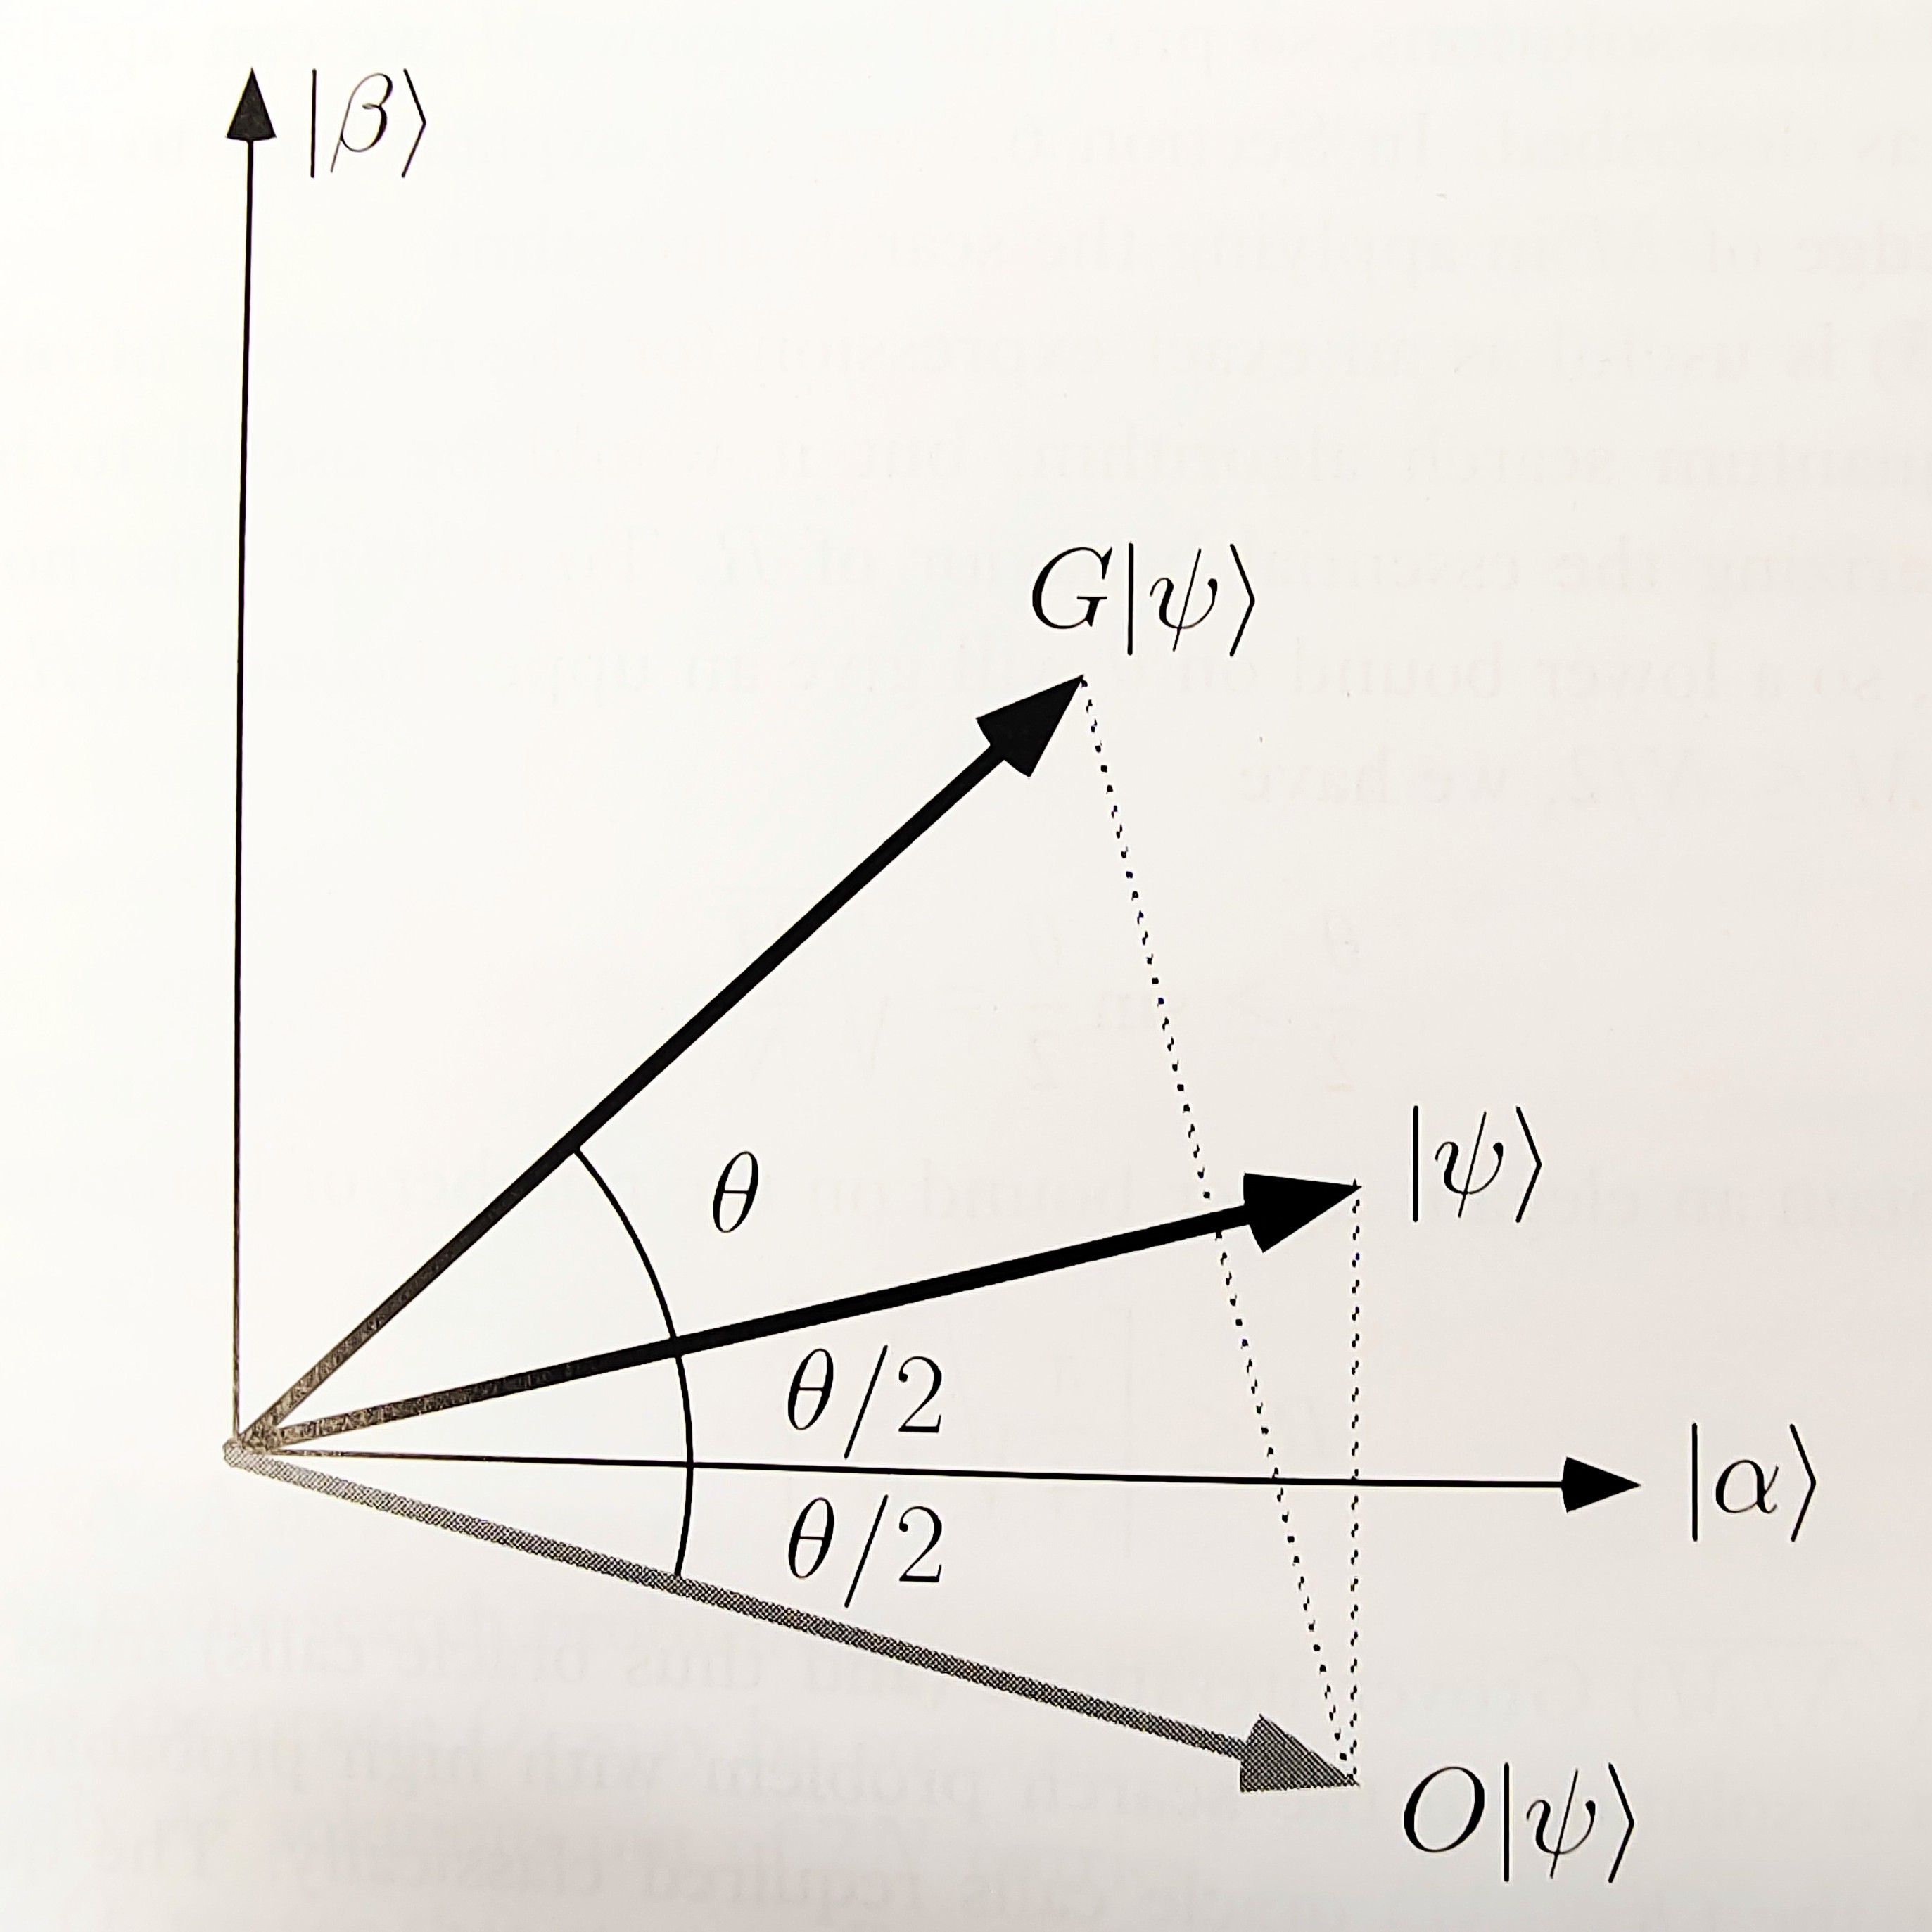
\includegraphics{figures/single_grover_iteration.jpg}
	\caption{Application Grover Oracle Operator(copyright Nielsen \& Chuang 2010)}
\end{figure}

The Grover operator applies the oracle operator \(O\) phase shift to
\(|\psi\rangle\), to mark the solution.\\
\(O|\psi\rangle\) is a reflection of the initial state vector
\(|\psi\rangle\) about the state \(|\alpha\rangle\).

The Grover algorithm then applies a \(2|\psi\rangle\langle\psi| - I\)
reflection about \(|\psi\rangle\).

The pair of reflections is guaranteed to leave the new state
\(G|\psi\rangle\) in the space spanned by \(|\alpha\rangle\) and
\(|\beta\rangle\).

    \hypertarget{qiskit-implementation}{%
\subsubsection*{QISKIT Implementation}\label{qiskit-implementation}}

In our set-up, using the QISKIT components, the Oracle marks the correct
solution by flipping the \emph{phase} of the correct state.\\
We will see that we do this by setting up a Unitary matrix operator,
with the phase flipped.

    \begin{tcolorbox}[breakable, size=fbox, boxrule=1pt, pad at break*=1mm,colback=cellbackground, colframe=cellborder]
\prompt{In}{incolor}{1}{\boxspacing}
\begin{Verbatim}[commandchars=\\\{\}]
\PY{k+kn}{import} \PY{n+nn}{numpy} \PY{k}{as} \PY{n+nn}{np}
\PY{k+kn}{from} \PY{n+nn}{qiskit} \PY{k+kn}{import} \PY{n}{QuantumCircuit}\PY{p}{,} \PY{n}{transpile}\PY{p}{,} \PY{n}{QuantumRegister}\PY{p}{,} \PY{n}{ClassicalRegister}
\PY{k+kn}{from} \PY{n+nn}{qiskit}\PY{n+nn}{.}\PY{n+nn}{visualization} \PY{k+kn}{import} \PY{n}{plot\PYZus{}histogram}
\PY{k+kn}{from} \PY{n+nn}{qiskit}\PY{n+nn}{.}\PY{n+nn}{circuit}\PY{n+nn}{.}\PY{n+nn}{library} \PY{k+kn}{import} \PY{n}{GroverOperator}
\PY{k+kn}{from} \PY{n+nn}{qiskit\PYZus{}aer} \PY{k+kn}{import} \PY{n}{AerSimulator}
\PY{k+kn}{import} \PY{n+nn}{matplotlib}\PY{n+nn}{.}\PY{n+nn}{pyplot} \PY{k}{as} \PY{n+nn}{plt}

\PY{c+c1}{\PYZsh{} Create oracle matrix}
\PY{n}{n} \PY{o}{=} \PY{l+m+mi}{4}
\PY{n}{solutions} \PY{o}{=} \PY{p}{[}\PY{l+m+mi}{3}\PY{p}{,} \PY{l+m+mi}{5}\PY{p}{]}
\PY{n}{size} \PY{o}{=} \PY{l+m+mi}{2} \PY{o}{*}\PY{o}{*} \PY{n}{n}
\PY{n}{oracle} \PY{o}{=} \PY{n}{np}\PY{o}{.}\PY{n}{eye}\PY{p}{(}\PY{n}{size}\PY{p}{)}
\PY{k}{for} \PY{n}{idx} \PY{o+ow}{in} \PY{n}{solutions}\PY{p}{:}
    \PY{n}{oracle}\PY{p}{[}\PY{n}{idx}\PY{p}{,} \PY{n}{idx}\PY{p}{]} \PY{o}{=} \PY{o}{\PYZhy{}}\PY{l+m+mi}{1}
\PY{n+nb}{print}\PY{p}{(}\PY{l+s+sa}{f}\PY{l+s+s2}{\PYZdq{}}\PY{l+s+s2}{With }\PY{l+s+si}{\PYZob{}}\PY{n}{n}\PY{l+s+si}{\PYZcb{}}\PY{l+s+s2}{ qubits, we have a hilbert space of size }\PY{l+s+si}{\PYZob{}}\PY{l+m+mi}{2}\PY{+w}{ }\PY{o}{*}\PY{o}{*}\PY{+w}{ }\PY{n}{n}\PY{l+s+si}{\PYZcb{}}\PY{l+s+s2}{\PYZdq{}}\PY{p}{)}
\PY{n+nb}{print}\PY{p}{(}\PY{n}{oracle}\PY{p}{)}

\PY{c+c1}{\PYZsh{} Convert to quantum circuit}
\PY{n}{oracle\PYZus{}circuit} \PY{o}{=} \PY{n}{QuantumCircuit}\PY{p}{(}\PY{n}{n}\PY{p}{)}
\PY{n}{oracle\PYZus{}circuit}\PY{o}{.}\PY{n}{unitary}\PY{p}{(}\PY{n}{oracle}\PY{p}{,} \PY{n+nb}{range}\PY{p}{(}\PY{n}{n}\PY{p}{)}\PY{p}{,} \PY{n}{label}\PY{o}{=}\PY{l+s+s2}{\PYZdq{}}\PY{l+s+s2}{Oracle}\PY{l+s+s2}{\PYZdq{}}\PY{p}{)}
\PY{n}{oracle\PYZus{}circuit}\PY{o}{.}\PY{n}{decompose}\PY{p}{(}\PY{p}{)}\PY{o}{.}\PY{n}{draw}\PY{p}{(}\PY{l+s+s2}{\PYZdq{}}\PY{l+s+s2}{mpl}\PY{l+s+s2}{\PYZdq{}}\PY{p}{)}
\end{Verbatim}
\end{tcolorbox}

    \begin{Verbatim}[commandchars=\\\{\}]
With 4 qubits, we have a hilbert space of size 16
[[ 1.  0.  0.  0.  0.  0.  0.  0.  0.  0.  0.  0.  0.  0.  0.  0.]
 [ 0.  1.  0.  0.  0.  0.  0.  0.  0.  0.  0.  0.  0.  0.  0.  0.]
 [ 0.  0.  1.  0.  0.  0.  0.  0.  0.  0.  0.  0.  0.  0.  0.  0.]
 [ 0.  0.  0. -1.  0.  0.  0.  0.  0.  0.  0.  0.  0.  0.  0.  0.]
 [ 0.  0.  0.  0.  1.  0.  0.  0.  0.  0.  0.  0.  0.  0.  0.  0.]
 [ 0.  0.  0.  0.  0. -1.  0.  0.  0.  0.  0.  0.  0.  0.  0.  0.]
 [ 0.  0.  0.  0.  0.  0.  1.  0.  0.  0.  0.  0.  0.  0.  0.  0.]
 [ 0.  0.  0.  0.  0.  0.  0.  1.  0.  0.  0.  0.  0.  0.  0.  0.]
 [ 0.  0.  0.  0.  0.  0.  0.  0.  1.  0.  0.  0.  0.  0.  0.  0.]
 [ 0.  0.  0.  0.  0.  0.  0.  0.  0.  1.  0.  0.  0.  0.  0.  0.]
 [ 0.  0.  0.  0.  0.  0.  0.  0.  0.  0.  1.  0.  0.  0.  0.  0.]
 [ 0.  0.  0.  0.  0.  0.  0.  0.  0.  0.  0.  1.  0.  0.  0.  0.]
 [ 0.  0.  0.  0.  0.  0.  0.  0.  0.  0.  0.  0.  1.  0.  0.  0.]
 [ 0.  0.  0.  0.  0.  0.  0.  0.  0.  0.  0.  0.  0.  1.  0.  0.]
 [ 0.  0.  0.  0.  0.  0.  0.  0.  0.  0.  0.  0.  0.  0.  1.  0.]
 [ 0.  0.  0.  0.  0.  0.  0.  0.  0.  0.  0.  0.  0.  0.  0.  1.]]
    \end{Verbatim}
 
            
\prompt{Out}{outcolor}{1}{}
    
    \begin{center}
    \adjustimage{max size={0.9\linewidth}{0.9\paperheight}}{figures/unit_3.3_grovers_algorithm_3_1.png}
    \end{center}
    { \hspace*{\fill} \\}
    

    \begin{tcolorbox}[breakable, size=fbox, boxrule=1pt, pad at break*=1mm,colback=cellbackground, colframe=cellborder]
\prompt{In}{incolor}{2}{\boxspacing}
\begin{Verbatim}[commandchars=\\\{\}]
\PY{c+c1}{\PYZsh{} Calculate optimal number of iterations}
\PY{n}{k} \PY{o}{=} \PY{n+nb}{max}\PY{p}{(}\PY{l+m+mi}{1}\PY{p}{,} \PY{n+nb}{int}\PY{p}{(}\PY{n}{np}\PY{o}{.}\PY{n}{floor}\PY{p}{(}\PY{p}{(}\PY{n}{np}\PY{o}{.}\PY{n}{pi} \PY{o}{/} \PY{l+m+mi}{4}\PY{p}{)} \PY{o}{*} \PY{n}{np}\PY{o}{.}\PY{n}{sqrt}\PY{p}{(}\PY{l+m+mi}{2} \PY{o}{*}\PY{o}{*} \PY{n}{n} \PY{o}{/} \PY{n+nb}{len}\PY{p}{(}\PY{n}{solutions}\PY{p}{)}\PY{p}{)}\PY{p}{)}\PY{p}{)}\PY{p}{,} \PY{l+m+mi}{0}\PY{p}{)}

\PY{c+c1}{\PYZsh{} Create quantum and classical registers}
\PY{n}{qn} \PY{o}{=} \PY{n}{QuantumRegister}\PY{p}{(}\PY{n}{n}\PY{p}{,} \PY{l+s+s1}{\PYZsq{}}\PY{l+s+s1}{qn}\PY{l+s+s1}{\PYZsq{}}\PY{p}{)}
\PY{n}{c} \PY{o}{=} \PY{n}{ClassicalRegister}\PY{p}{(}\PY{n}{n}\PY{p}{,} \PY{l+s+s1}{\PYZsq{}}\PY{l+s+s1}{c}\PY{l+s+s1}{\PYZsq{}}\PY{p}{)}
\PY{n}{qc} \PY{o}{=} \PY{n}{QuantumCircuit}\PY{p}{(}\PY{n}{qn}\PY{p}{,} \PY{n}{c}\PY{p}{)}

\PY{c+c1}{\PYZsh{} Initialize superposition}
\PY{n}{qc}\PY{o}{.}\PY{n}{h}\PY{p}{(}\PY{n}{qn}\PY{p}{)}
        
\PY{c+c1}{\PYZsh{} Create the grover operator to apply the reflections, and apply for k iterations}
\PY{n}{grover\PYZus{}operator} \PY{o}{=} \PY{n}{GroverOperator}\PY{p}{(}\PY{n}{oracle\PYZus{}circuit}\PY{p}{)}

\PY{k}{for} \PY{n}{\PYZus{}} \PY{o+ow}{in} \PY{n+nb}{range}\PY{p}{(}\PY{n}{k}\PY{p}{)}\PY{p}{:}
    \PY{n}{qc}\PY{o}{.}\PY{n}{append}\PY{p}{(}\PY{n}{grover\PYZus{}operator}\PY{p}{,} \PY{n}{qn}\PY{p}{)}

\PY{c+c1}{\PYZsh{} Measure results}
\PY{n}{qc}\PY{o}{.}\PY{n}{measure}\PY{p}{(}\PY{n}{qn}\PY{p}{,} \PY{n}{c}\PY{p}{)}
\PY{n}{qc}\PY{o}{.}\PY{n}{draw}\PY{p}{(}\PY{l+s+s2}{\PYZdq{}}\PY{l+s+s2}{mpl}\PY{l+s+s2}{\PYZdq{}}\PY{p}{)}
\end{Verbatim}
\end{tcolorbox}
 
            
\prompt{Out}{outcolor}{2}{}
    
    \begin{center}
    \adjustimage{max size={0.9\linewidth}{0.9\paperheight}}{figures/unit_3.3_grovers_algorithm_4_0.png}
    \end{center}
    { \hspace*{\fill} \\}
    

    \begin{tcolorbox}[breakable, size=fbox, boxrule=1pt, pad at break*=1mm,colback=cellbackground, colframe=cellborder]
\prompt{In}{incolor}{3}{\boxspacing}
\begin{Verbatim}[commandchars=\\\{\}]
\PY{n+nb}{print}\PY{p}{(}\PY{l+s+sa}{f}\PY{l+s+s2}{\PYZdq{}}\PY{l+s+s2}{Simple Grover}\PY{l+s+s2}{\PYZsq{}}\PY{l+s+s2}{s Algorithm Circuit}\PY{l+s+se}{\PYZbs{}n}\PY{l+s+s2}{\PYZdq{}}
      \PY{l+s+sa}{f}\PY{l+s+s2}{\PYZdq{}}\PY{l+s+s2}{Searching for }\PY{l+s+si}{\PYZob{}}\PY{n+nb}{len}\PY{p}{(}\PY{n}{solutions}\PY{p}{)}\PY{l+s+si}{\PYZcb{}}\PY{l+s+s2}{ solution}\PY{l+s+si}{\PYZob{}}\PY{l+s+s1}{\PYZsq{}}\PY{l+s+s1}{s}\PY{l+s+s1}{\PYZsq{}}\PY{+w}{ }\PY{k}{if}\PY{+w}{ }\PY{n+nb}{len}\PY{p}{(}\PY{n}{solutions}\PY{p}{)}\PY{o}{\PYZgt{}}\PY{l+m+mi}{1}\PY{+w}{ }\PY{k}{else}\PY{+w}{ }\PY{l+s+s1}{\PYZsq{}}\PY{l+s+s1}{\PYZsq{}}\PY{l+s+si}{\PYZcb{}}\PY{l+s+s2}{ }\PY{l+s+s2}{\PYZdq{}}
      \PY{l+s+sa}{f}\PY{l+s+s2}{\PYZdq{}}\PY{l+s+s2}{in }\PY{l+s+si}{\PYZob{}}\PY{l+m+mi}{2}\PY{o}{*}\PY{o}{*}\PY{n}{n}\PY{l+s+si}{\PYZcb{}}\PY{l+s+s2}{ states}\PY{l+s+se}{\PYZbs{}n}\PY{l+s+s2}{\PYZdq{}}
      \PY{l+s+sa}{f}\PY{l+s+s2}{\PYZdq{}}\PY{l+s+s2}{Number of iterations: }\PY{l+s+si}{\PYZob{}}\PY{n}{qc}\PY{o}{.}\PY{n}{count\PYZus{}ops}\PY{p}{(}\PY{p}{)}\PY{o}{.}\PY{n}{get}\PY{p}{(}\PY{l+s+s1}{\PYZsq{}}\PY{l+s+s1}{Q}\PY{l+s+s1}{\PYZsq{}}\PY{p}{,}\PY{+w}{ }\PY{l+m+mi}{0}\PY{p}{)}\PY{l+s+si}{\PYZcb{}}\PY{l+s+se}{\PYZbs{}n}\PY{l+s+s2}{\PYZdq{}}\PY{p}{)}

\PY{n+nb}{print}\PY{p}{(}\PY{l+s+sa}{f}\PY{l+s+s2}{\PYZdq{}}\PY{l+s+s2}{Circuit Statistics:}\PY{l+s+se}{\PYZbs{}n}\PY{l+s+s2}{\PYZdq{}}
      \PY{l+s+sa}{f}\PY{l+s+s2}{\PYZdq{}}\PY{l+s+s2}{Qubits: }\PY{l+s+si}{\PYZob{}}\PY{n}{n}\PY{l+s+si}{\PYZcb{}}\PY{l+s+se}{\PYZbs{}n}\PY{l+s+s2}{\PYZdq{}}
      \PY{l+s+sa}{f}\PY{l+s+s2}{\PYZdq{}}\PY{l+s+s2}{Gates: }\PY{l+s+si}{\PYZob{}}\PY{n+nb}{sum}\PY{p}{(}\PY{n}{qc}\PY{o}{.}\PY{n}{count\PYZus{}ops}\PY{p}{(}\PY{p}{)}\PY{o}{.}\PY{n}{values}\PY{p}{(}\PY{p}{)}\PY{p}{)}\PY{l+s+si}{\PYZcb{}}\PY{l+s+se}{\PYZbs{}n}\PY{l+s+s2}{\PYZdq{}}
      \PY{l+s+sa}{f}\PY{l+s+s2}{\PYZdq{}}\PY{l+s+s2}{Depth: }\PY{l+s+si}{\PYZob{}}\PY{n}{qc}\PY{o}{.}\PY{n}{depth}\PY{p}{(}\PY{p}{)}\PY{l+s+si}{\PYZcb{}}\PY{l+s+s2}{\PYZdq{}}\PY{p}{)}

\PY{c+c1}{\PYZsh{} Run simulation}
\PY{n}{simulator} \PY{o}{=} \PY{n}{AerSimulator}\PY{p}{(}\PY{p}{)}
\PY{n}{qc\PYZus{}t} \PY{o}{=} \PY{n}{transpile}\PY{p}{(}\PY{n}{qc}\PY{p}{,} \PY{n}{simulator}\PY{p}{)}
\PY{n}{result} \PY{o}{=} \PY{n}{simulator}\PY{o}{.}\PY{n}{run}\PY{p}{(}\PY{n}{qc\PYZus{}t}\PY{p}{,} \PY{n}{shots}\PY{o}{=}\PY{l+m+mi}{300}\PY{p}{)}\PY{o}{.}\PY{n}{result}\PY{p}{(}\PY{p}{)}
\PY{n}{counts} \PY{o}{=} \PY{n}{result}\PY{o}{.}\PY{n}{get\PYZus{}counts}\PY{p}{(}\PY{p}{)}

\PY{n}{plot\PYZus{}histogram}\PY{p}{(}\PY{n}{counts}\PY{p}{)}
\end{Verbatim}
\end{tcolorbox}

    \begin{Verbatim}[commandchars=\\\{\}]
Simple Grover's Algorithm Circuit
Searching for 2 solutions in 16 states
Number of iterations: 2

Circuit Statistics:
Qubits: 4
Gates: 10
Depth: 4
    \end{Verbatim}
 
            
\prompt{Out}{outcolor}{3}{}
    
    \begin{center}
    \adjustimage{max size={0.9\linewidth}{0.9\paperheight}}{figures/unit_3.3_grovers_algorithm_5_1.png}
    \end{center}
    { \hspace*{\fill} \\}
    

    \hypertarget{running-grovers-algorithm}{%
\subsection*{Running Grover's
algorithm}\label{running-grovers-algorithm}}

This is the code from the IBM tutorial
\href{https://qiskit-community.github.io/qiskit-algorithms/tutorials/06_grover.html}{IBM
QISKIT Grover notebook source}

Specify an oracle for the circuit of Grover's algorithm.

    \begin{tcolorbox}[breakable, size=fbox, boxrule=1pt, pad at break*=1mm,colback=cellbackground, colframe=cellborder]
\prompt{In}{incolor}{4}{\boxspacing}
\begin{Verbatim}[commandchars=\\\{\}]
\PY{k+kn}{from} \PY{n+nn}{qiskit} \PY{k+kn}{import} \PY{n}{QuantumCircuit}
\PY{k+kn}{from} \PY{n+nn}{qiskit\PYZus{}algorithms} \PY{k+kn}{import} \PY{n}{AmplificationProblem}

\PY{c+c1}{\PYZsh{} the state we desire to find is \PYZsq{}11\PYZsq{}}
\PY{n}{good\PYZus{}state} \PY{o}{=} \PY{p}{[}\PY{l+s+s2}{\PYZdq{}}\PY{l+s+s2}{11}\PY{l+s+s2}{\PYZdq{}}\PY{p}{]}

\PY{c+c1}{\PYZsh{} specify the oracle that marks the state \PYZsq{}11\PYZsq{} as a good solution}
\PY{n}{oracle} \PY{o}{=} \PY{n}{QuantumCircuit}\PY{p}{(}\PY{l+m+mi}{2}\PY{p}{)}
\PY{n}{oracle}\PY{o}{.}\PY{n}{cz}\PY{p}{(}\PY{l+m+mi}{0}\PY{p}{,} \PY{l+m+mi}{1}\PY{p}{)}

\PY{c+c1}{\PYZsh{} define Grover\PYZsq{}s algorithm}
\PY{n}{problem} \PY{o}{=} \PY{n}{AmplificationProblem}\PY{p}{(}\PY{n}{oracle}\PY{p}{,} \PY{n}{is\PYZus{}good\PYZus{}state}\PY{o}{=}\PY{n}{good\PYZus{}state}\PY{p}{)}

\PY{c+c1}{\PYZsh{} now we can have a look at the Grover operator that is used in running the algorithm}
\PY{c+c1}{\PYZsh{} (Algorithm circuits are wrapped in a gate to appear in composition as a block}
\PY{c+c1}{\PYZsh{} so we have to decompose() the op to see it expanded into its component gates.)}
\PY{n}{problem}\PY{o}{.}\PY{n}{grover\PYZus{}operator}\PY{o}{.}\PY{n}{decompose}\PY{p}{(}\PY{p}{)}\PY{o}{.}\PY{n}{draw}\PY{p}{(}\PY{n}{output}\PY{o}{=}\PY{l+s+s2}{\PYZdq{}}\PY{l+s+s2}{mpl}\PY{l+s+s2}{\PYZdq{}}\PY{p}{)}
\end{Verbatim}
\end{tcolorbox}
 
            
\prompt{Out}{outcolor}{4}{}
    
    \begin{center}
    \adjustimage{max size={0.9\linewidth}{0.9\paperheight}}{figures/unit_3.3_grovers_algorithm_7_0.png}
    \end{center}
    { \hspace*{\fill} \\}
    

    Specify a backend to execute the circuits. Notice that we find a ``good
state'' in the `top\_measurement'.

    \begin{tcolorbox}[breakable, size=fbox, boxrule=1pt, pad at break*=1mm,colback=cellbackground, colframe=cellborder]
\prompt{In}{incolor}{5}{\boxspacing}
\begin{Verbatim}[commandchars=\\\{\}]
\PY{k+kn}{from} \PY{n+nn}{qiskit\PYZus{}algorithms} \PY{k+kn}{import} \PY{n}{Grover}
\PY{k+kn}{from} \PY{n+nn}{qiskit}\PY{n+nn}{.}\PY{n+nn}{primitives} \PY{k+kn}{import} \PY{n}{Sampler}

\PY{n}{grover} \PY{o}{=} \PY{n}{Grover}\PY{p}{(}\PY{n}{sampler}\PY{o}{=}\PY{n}{Sampler}\PY{p}{(}\PY{p}{)}\PY{p}{)}
\PY{n}{result} \PY{o}{=} \PY{n}{grover}\PY{o}{.}\PY{n}{amplify}\PY{p}{(}\PY{n}{problem}\PY{p}{)}
\PY{n+nb}{print}\PY{p}{(}\PY{l+s+s2}{\PYZdq{}}\PY{l+s+s2}{Result type:}\PY{l+s+s2}{\PYZdq{}}\PY{p}{,} \PY{n+nb}{type}\PY{p}{(}\PY{n}{result}\PY{p}{)}\PY{p}{)}
\PY{n+nb}{print}\PY{p}{(}\PY{p}{)}
\PY{n+nb}{print}\PY{p}{(}\PY{l+s+s2}{\PYZdq{}}\PY{l+s+s2}{Success!}\PY{l+s+s2}{\PYZdq{}} \PY{k}{if} \PY{n}{result}\PY{o}{.}\PY{n}{oracle\PYZus{}evaluation} \PY{k}{else} \PY{l+s+s2}{\PYZdq{}}\PY{l+s+s2}{Failure!}\PY{l+s+s2}{\PYZdq{}}\PY{p}{)}
\PY{n+nb}{print}\PY{p}{(}\PY{l+s+s2}{\PYZdq{}}\PY{l+s+s2}{Top measurement:}\PY{l+s+s2}{\PYZdq{}}\PY{p}{,} \PY{n}{result}\PY{o}{.}\PY{n}{top\PYZus{}measurement}\PY{p}{)}
\end{Verbatim}
\end{tcolorbox}

    \begin{Verbatim}[commandchars=\\\{\}]
Result type: <class
'qiskit\_algorithms.amplitude\_amplifiers.grover.GroverResult'>

Success!
Top measurement: 11
    \end{Verbatim}

    \begin{Verbatim}[commandchars=\\\{\}]
/tmp/ipykernel\_292492/4134062562.py:4: DeprecationWarning: The class
``qiskit.primitives.sampler.Sampler`` is deprecated as of qiskit 1.2. It will be
removed no earlier than 3 months after the release date. All implementations of
the `BaseSamplerV1` interface have been deprecated in favor of their V2
counterparts. The V2 alternative for the `Sampler` class is
`StatevectorSampler`.
  grover = Grover(sampler=Sampler())
    \end{Verbatim}

    We can use different QISKIT components as an Oracle. Here is the same
example, but using the \texttt{StateVector} instead.

    \begin{tcolorbox}[breakable, size=fbox, boxrule=1pt, pad at break*=1mm,colback=cellbackground, colframe=cellborder]
\prompt{In}{incolor}{6}{\boxspacing}
\begin{Verbatim}[commandchars=\\\{\}]
\PY{k+kn}{from} \PY{n+nn}{qiskit}\PY{n+nn}{.}\PY{n+nn}{quantum\PYZus{}info} \PY{k+kn}{import} \PY{n}{Statevector}

\PY{n}{oracle} \PY{o}{=} \PY{n}{Statevector}\PY{o}{.}\PY{n}{from\PYZus{}label}\PY{p}{(}\PY{l+s+s2}{\PYZdq{}}\PY{l+s+s2}{11}\PY{l+s+s2}{\PYZdq{}}\PY{p}{)}
\PY{n}{problem} \PY{o}{=} \PY{n}{AmplificationProblem}\PY{p}{(}\PY{n}{oracle}\PY{p}{,} \PY{n}{is\PYZus{}good\PYZus{}state}\PY{o}{=}\PY{p}{[}\PY{l+s+s2}{\PYZdq{}}\PY{l+s+s2}{11}\PY{l+s+s2}{\PYZdq{}}\PY{p}{]}\PY{p}{)}

\PY{n}{grover} \PY{o}{=} \PY{n}{Grover}\PY{p}{(}\PY{n}{sampler}\PY{o}{=}\PY{n}{Sampler}\PY{p}{(}\PY{p}{)}\PY{p}{)}
\PY{n}{result} \PY{o}{=} \PY{n}{grover}\PY{o}{.}\PY{n}{amplify}\PY{p}{(}\PY{n}{problem}\PY{p}{)}
\PY{n+nb}{print}\PY{p}{(}\PY{l+s+s2}{\PYZdq{}}\PY{l+s+s2}{Result type:}\PY{l+s+s2}{\PYZdq{}}\PY{p}{,} \PY{n+nb}{type}\PY{p}{(}\PY{n}{result}\PY{p}{)}\PY{p}{)}
\PY{n+nb}{print}\PY{p}{(}\PY{p}{)}
\PY{n+nb}{print}\PY{p}{(}\PY{l+s+s2}{\PYZdq{}}\PY{l+s+s2}{Success!}\PY{l+s+s2}{\PYZdq{}} \PY{k}{if} \PY{n}{result}\PY{o}{.}\PY{n}{oracle\PYZus{}evaluation} \PY{k}{else} \PY{l+s+s2}{\PYZdq{}}\PY{l+s+s2}{Failure!}\PY{l+s+s2}{\PYZdq{}}\PY{p}{)}
\PY{n+nb}{print}\PY{p}{(}\PY{l+s+s2}{\PYZdq{}}\PY{l+s+s2}{Top measurement:}\PY{l+s+s2}{\PYZdq{}}\PY{p}{,} \PY{n}{result}\PY{o}{.}\PY{n}{top\PYZus{}measurement}\PY{p}{)}
\end{Verbatim}
\end{tcolorbox}

    \begin{Verbatim}[commandchars=\\\{\}]
Result type: <class
'qiskit\_algorithms.amplitude\_amplifiers.grover.GroverResult'>

Success!
Top measurement: 11
    \end{Verbatim}

    \begin{Verbatim}[commandchars=\\\{\}]
/tmp/ipykernel\_292492/1906973721.py:6: DeprecationWarning: The class
``qiskit.primitives.sampler.Sampler`` is deprecated as of qiskit 1.2. It will be
removed no earlier than 3 months after the release date. All implementations of
the `BaseSamplerV1` interface have been deprecated in favor of their V2
counterparts. The V2 alternative for the `Sampler` class is
`StatevectorSampler`.
  grover = Grover(sampler=Sampler())
    \end{Verbatim}

    Internally, the statevector is mapped to a quantum circuit:

    \begin{tcolorbox}[breakable, size=fbox, boxrule=1pt, pad at break*=1mm,colback=cellbackground, colframe=cellborder]
\prompt{In}{incolor}{7}{\boxspacing}
\begin{Verbatim}[commandchars=\\\{\}]
\PY{n}{problem}\PY{o}{.}\PY{n}{grover\PYZus{}operator}\PY{o}{.}\PY{n}{oracle}\PY{o}{.}\PY{n}{decompose}\PY{p}{(}\PY{p}{)}\PY{o}{.}\PY{n}{draw}\PY{p}{(}\PY{n}{output}\PY{o}{=}\PY{l+s+s2}{\PYZdq{}}\PY{l+s+s2}{mpl}\PY{l+s+s2}{\PYZdq{}}\PY{p}{)}
\end{Verbatim}
\end{tcolorbox}
 
            
\prompt{Out}{outcolor}{7}{}
    
    \begin{center}
    \adjustimage{max size={0.9\linewidth}{0.9\paperheight}}{figures/unit_3.3_grovers_algorithm_13_0.png}
    \end{center}
    { \hspace*{\fill} \\}
    

    Qiskit allows for an easy construction of more complex oracles.\\
\texttt{PhaseOracle} is used for parsing logical expressions such as
`\textasciitilde a \textbar{} b', and is useful for solving 3-SAT
problems.

Here we use the \texttt{PhaseOracle} for the simple example of finding
the state \(|11>\), which corresponds to `a \& b'

It does this by implementing a phase flip when the state is \(|11>\).

    \begin{tcolorbox}[breakable, size=fbox, boxrule=1pt, pad at break*=1mm,colback=cellbackground, colframe=cellborder]
\prompt{In}{incolor}{8}{\boxspacing}
\begin{Verbatim}[commandchars=\\\{\}]
\PY{k+kn}{from} \PY{n+nn}{qiskit}\PY{n+nn}{.}\PY{n+nn}{circuit}\PY{n+nn}{.}\PY{n+nn}{library}\PY{n+nn}{.}\PY{n+nn}{phase\PYZus{}oracle} \PY{k+kn}{import} \PY{n}{PhaseOracle}
\PY{k+kn}{from} \PY{n+nn}{qiskit}\PY{n+nn}{.}\PY{n+nn}{exceptions} \PY{k+kn}{import} \PY{n}{MissingOptionalLibraryError}

\PY{c+c1}{\PYZsh{} `Oracle` (`PhaseOracle`) as the `oracle` argument}
\PY{n}{expression} \PY{o}{=} \PY{l+s+s2}{\PYZdq{}}\PY{l+s+s2}{(a \PYZam{} b)}\PY{l+s+s2}{\PYZdq{}}
\PY{k}{try}\PY{p}{:}
    \PY{n}{oracle} \PY{o}{=} \PY{n}{PhaseOracle}\PY{p}{(}\PY{n}{expression}\PY{p}{)}
    \PY{n}{problem} \PY{o}{=} \PY{n}{AmplificationProblem}\PY{p}{(}\PY{n}{oracle}\PY{p}{)}
    \PY{n}{display}\PY{p}{(}\PY{n}{problem}\PY{o}{.}\PY{n}{grover\PYZus{}operator}\PY{o}{.}\PY{n}{oracle}\PY{o}{.}\PY{n}{decompose}\PY{p}{(}\PY{p}{)}\PY{o}{.}\PY{n}{draw}\PY{p}{(}\PY{n}{output}\PY{o}{=}\PY{l+s+s2}{\PYZdq{}}\PY{l+s+s2}{mpl}\PY{l+s+s2}{\PYZdq{}}\PY{p}{)}\PY{p}{)}
\PY{k}{except} \PY{n}{MissingOptionalLibraryError} \PY{k}{as} \PY{n}{ex}\PY{p}{:}
    \PY{n+nb}{print}\PY{p}{(}\PY{n}{ex}\PY{p}{)}
\end{Verbatim}
\end{tcolorbox}

    \begin{center}
    \adjustimage{max size={0.9\linewidth}{0.9\paperheight}}{figures/unit_3.3_grovers_algorithm_15_0.png}
    \end{center}
    { \hspace*{\fill} \\}
    
    \hypertarget{amplitude-amplification}{%
\subsubsection*{Amplitude Amplification}\label{amplitude-amplification}}

Grover's algorithm uses Hadamard gates to create the uniform
superposition of all the states at the beginning of the Grover operator
. If some information on the good states is available, it might be
useful to not start in a uniform superposition but only initialize
specific states. This, generalized, version of Grover's algorithm is
referred to Amplitude Amplification.

    \begin{tcolorbox}[breakable, size=fbox, boxrule=1pt, pad at break*=1mm,colback=cellbackground, colframe=cellborder]
\prompt{In}{incolor}{9}{\boxspacing}
\begin{Verbatim}[commandchars=\\\{\}]
\PY{k+kn}{import} \PY{n+nn}{numpy} \PY{k}{as} \PY{n+nn}{np}

\PY{c+c1}{\PYZsh{} Specifying `state\PYZus{}preparation`}
\PY{c+c1}{\PYZsh{} to prepare a superposition of |01\PYZgt{}, |10\PYZgt{}, and |11\PYZgt{}}
\PY{n}{oracle} \PY{o}{=} \PY{n}{QuantumCircuit}\PY{p}{(}\PY{l+m+mi}{3}\PY{p}{)}
\PY{n}{oracle}\PY{o}{.}\PY{n}{ccz}\PY{p}{(}\PY{l+m+mi}{0}\PY{p}{,} \PY{l+m+mi}{1}\PY{p}{,} \PY{l+m+mi}{2}\PY{p}{)}

\PY{n}{theta} \PY{o}{=} \PY{l+m+mi}{2} \PY{o}{*} \PY{n}{np}\PY{o}{.}\PY{n}{arccos}\PY{p}{(}\PY{l+m+mi}{1} \PY{o}{/} \PY{n}{np}\PY{o}{.}\PY{n}{sqrt}\PY{p}{(}\PY{l+m+mi}{3}\PY{p}{)}\PY{p}{)}
\PY{n}{state\PYZus{}preparation} \PY{o}{=} \PY{n}{QuantumCircuit}\PY{p}{(}\PY{l+m+mi}{3}\PY{p}{)}
\PY{n}{state\PYZus{}preparation}\PY{o}{.}\PY{n}{ry}\PY{p}{(}\PY{n}{theta}\PY{p}{,} \PY{l+m+mi}{0}\PY{p}{)}          \PY{c+c1}{\PYZsh{} Single\PYZhy{}qubit rotation about the Y axis.}
\PY{n}{state\PYZus{}preparation}\PY{o}{.}\PY{n}{ch}\PY{p}{(}\PY{l+m+mi}{0}\PY{p}{,} \PY{l+m+mi}{1}\PY{p}{)}              \PY{c+c1}{\PYZsh{} Applies a Hadamard on the target qubit if the control is in the ∣1⟩ state.}
\PY{n}{state\PYZus{}preparation}\PY{o}{.}\PY{n}{x}\PY{p}{(}\PY{l+m+mi}{1}\PY{p}{)}
\PY{n}{state\PYZus{}preparation}\PY{o}{.}\PY{n}{h}\PY{p}{(}\PY{l+m+mi}{2}\PY{p}{)}

\PY{c+c1}{\PYZsh{} we only care about the first two bits being in state 1, thus add both possibilities for the last qubit}
\PY{n}{problem} \PY{o}{=} \PY{n}{AmplificationProblem}\PY{p}{(}
    \PY{n}{oracle}\PY{p}{,} \PY{n}{state\PYZus{}preparation}\PY{o}{=}\PY{n}{state\PYZus{}preparation}\PY{p}{,} \PY{n}{is\PYZus{}good\PYZus{}state}\PY{o}{=}\PY{p}{[}\PY{l+s+s2}{\PYZdq{}}\PY{l+s+s2}{110}\PY{l+s+s2}{\PYZdq{}}\PY{p}{,} \PY{l+s+s2}{\PYZdq{}}\PY{l+s+s2}{111}\PY{l+s+s2}{\PYZdq{}}\PY{p}{]}
\PY{p}{)}

\PY{c+c1}{\PYZsh{} state\PYZus{}preparation}
\PY{n+nb}{print}\PY{p}{(}\PY{l+s+s2}{\PYZdq{}}\PY{l+s+s2}{state preparation circuit:}\PY{l+s+s2}{\PYZdq{}}\PY{p}{)}
\PY{n}{problem}\PY{o}{.}\PY{n}{grover\PYZus{}operator}\PY{o}{.}\PY{n}{state\PYZus{}preparation}\PY{o}{.}\PY{n}{draw}\PY{p}{(}\PY{n}{output}\PY{o}{=}\PY{l+s+s2}{\PYZdq{}}\PY{l+s+s2}{mpl}\PY{l+s+s2}{\PYZdq{}}\PY{p}{)}
\end{Verbatim}
\end{tcolorbox}

    \begin{Verbatim}[commandchars=\\\{\}]
state preparation circuit:
    \end{Verbatim}
 
            
\prompt{Out}{outcolor}{9}{}
    
    \begin{center}
    \adjustimage{max size={0.9\linewidth}{0.9\paperheight}}{figures/unit_3.3_grovers_algorithm_17_1.png}
    \end{center}
    { \hspace*{\fill} \\}
    

    \begin{tcolorbox}[breakable, size=fbox, boxrule=1pt, pad at break*=1mm,colback=cellbackground, colframe=cellborder]
\prompt{In}{incolor}{10}{\boxspacing}
\begin{Verbatim}[commandchars=\\\{\}]
\PY{k+kn}{from} \PY{n+nn}{qiskit}\PY{n+nn}{.}\PY{n+nn}{visualization} \PY{k+kn}{import} \PY{n}{plot\PYZus{}bloch\PYZus{}multivector}
\PY{n}{state} \PY{o}{=} \PY{n}{Statevector}\PY{p}{(}\PY{n}{state\PYZus{}preparation}\PY{p}{)}
\PY{n}{plot\PYZus{}bloch\PYZus{}multivector}\PY{p}{(}\PY{n}{state}\PY{p}{)}
\end{Verbatim}
\end{tcolorbox}
 
            
\prompt{Out}{outcolor}{10}{}
    
    \begin{center}
    \adjustimage{max size={0.9\linewidth}{0.9\paperheight}}{figures/unit_3.3_grovers_algorithm_18_0.png}
    \end{center}
    { \hspace*{\fill} \\}
    

    \begin{tcolorbox}[breakable, size=fbox, boxrule=1pt, pad at break*=1mm,colback=cellbackground, colframe=cellborder]
\prompt{In}{incolor}{11}{\boxspacing}
\begin{Verbatim}[commandchars=\\\{\}]
\PY{n}{grover} \PY{o}{=} \PY{n}{Grover}\PY{p}{(}\PY{n}{sampler}\PY{o}{=}\PY{n}{Sampler}\PY{p}{(}\PY{p}{)}\PY{p}{)}
\PY{n}{result} \PY{o}{=} \PY{n}{grover}\PY{o}{.}\PY{n}{amplify}\PY{p}{(}\PY{n}{problem}\PY{p}{)}
\PY{n+nb}{print}\PY{p}{(}\PY{l+s+s2}{\PYZdq{}}\PY{l+s+s2}{Success!}\PY{l+s+s2}{\PYZdq{}} \PY{k}{if} \PY{n}{result}\PY{o}{.}\PY{n}{oracle\PYZus{}evaluation} \PY{k}{else} \PY{l+s+s2}{\PYZdq{}}\PY{l+s+s2}{Failure!}\PY{l+s+s2}{\PYZdq{}}\PY{p}{)}
\PY{n+nb}{print}\PY{p}{(}\PY{l+s+s2}{\PYZdq{}}\PY{l+s+s2}{Top measurement:}\PY{l+s+s2}{\PYZdq{}}\PY{p}{,} \PY{n}{result}\PY{o}{.}\PY{n}{top\PYZus{}measurement}\PY{p}{)}
\end{Verbatim}
\end{tcolorbox}

    \begin{Verbatim}[commandchars=\\\{\}]
Success!
Top measurement: 111
    \end{Verbatim}

    \begin{Verbatim}[commandchars=\\\{\}]
/tmp/ipykernel\_292492/336064450.py:1: DeprecationWarning: The class
``qiskit.primitives.sampler.Sampler`` is deprecated as of qiskit 1.2. It will be
removed no earlier than 3 months after the release date. All implementations of
the `BaseSamplerV1` interface have been deprecated in favor of their V2
counterparts. The V2 alternative for the `Sampler` class is
`StatevectorSampler`.
  grover = Grover(sampler=Sampler())
    \end{Verbatim}

    \hypertarget{flexibilty}{%
\paragraph{Flexibilty}\label{flexibilty}}

As we saw at the top of the notebook, it is also possible to specify the
entire Grover operator by setting the grover\_operator argument.

    \begin{tcolorbox}[breakable, size=fbox, boxrule=1pt, pad at break*=1mm,colback=cellbackground, colframe=cellborder]
\prompt{In}{incolor}{12}{\boxspacing}
\begin{Verbatim}[commandchars=\\\{\}]
\PY{n}{oracle} \PY{o}{=} \PY{n}{QuantumCircuit}\PY{p}{(}\PY{l+m+mi}{5}\PY{p}{)}
\PY{n}{oracle}\PY{o}{.}\PY{n}{ccz}\PY{p}{(}\PY{l+m+mi}{0}\PY{p}{,} \PY{l+m+mi}{1}\PY{p}{,} \PY{l+m+mi}{2}\PY{p}{)}             \PY{c+c1}{\PYZsh{} flips the phase of the target qubit if the control qubits are in the ∣11⟩ state.}
\PY{n}{oracle}\PY{o}{.}\PY{n}{draw}\PY{p}{(}\PY{n}{output}\PY{o}{=}\PY{l+s+s2}{\PYZdq{}}\PY{l+s+s2}{mpl}\PY{l+s+s2}{\PYZdq{}}\PY{p}{)}
\end{Verbatim}
\end{tcolorbox}
 
            
\prompt{Out}{outcolor}{12}{}
    
    \begin{center}
    \adjustimage{max size={0.9\linewidth}{0.9\paperheight}}{figures/unit_3.3_grovers_algorithm_21_0.png}
    \end{center}
    { \hspace*{\fill} \\}
    

    \begin{tcolorbox}[breakable, size=fbox, boxrule=1pt, pad at break*=1mm,colback=cellbackground, colframe=cellborder]
\prompt{In}{incolor}{13}{\boxspacing}
\begin{Verbatim}[commandchars=\\\{\}]
\PY{k+kn}{from} \PY{n+nn}{qiskit}\PY{n+nn}{.}\PY{n+nn}{circuit}\PY{n+nn}{.}\PY{n+nn}{library} \PY{k+kn}{import} \PY{n}{GroverOperator}

\PY{n}{grover\PYZus{}op} \PY{o}{=} \PY{n}{GroverOperator}\PY{p}{(}\PY{n}{oracle}\PY{p}{,} \PY{n}{insert\PYZus{}barriers}\PY{o}{=}\PY{k+kc}{True}\PY{p}{)}
\PY{n}{grover\PYZus{}op}\PY{o}{.}\PY{n}{decompose}\PY{p}{(}\PY{p}{)}\PY{o}{.}\PY{n}{draw}\PY{p}{(}\PY{n}{output}\PY{o}{=}\PY{l+s+s2}{\PYZdq{}}\PY{l+s+s2}{mpl}\PY{l+s+s2}{\PYZdq{}}\PY{p}{)}
\end{Verbatim}
\end{tcolorbox}
 
            
\prompt{Out}{outcolor}{13}{}
    
    \begin{center}
    \adjustimage{max size={0.9\linewidth}{0.9\paperheight}}{figures/unit_3.3_grovers_algorithm_22_0.png}
    \end{center}
    { \hspace*{\fill} \\}
    

    But we know that we only need to consider the first three:

    \begin{tcolorbox}[breakable, size=fbox, boxrule=1pt, pad at break*=1mm,colback=cellbackground, colframe=cellborder]
\prompt{In}{incolor}{14}{\boxspacing}
\begin{Verbatim}[commandchars=\\\{\}]
\PY{n}{grover\PYZus{}op} \PY{o}{=} \PY{n}{GroverOperator}\PY{p}{(}\PY{n}{oracle}\PY{p}{,} \PY{n}{reflection\PYZus{}qubits}\PY{o}{=}\PY{p}{[}\PY{l+m+mi}{0}\PY{p}{,} \PY{l+m+mi}{1}\PY{p}{,} \PY{l+m+mi}{2}\PY{p}{]}\PY{p}{,} \PY{n}{insert\PYZus{}barriers}\PY{o}{=}\PY{k+kc}{True}\PY{p}{)}
\PY{n}{grover\PYZus{}op}\PY{o}{.}\PY{n}{decompose}\PY{p}{(}\PY{p}{)}\PY{o}{.}\PY{n}{draw}\PY{p}{(}\PY{n}{output}\PY{o}{=}\PY{l+s+s2}{\PYZdq{}}\PY{l+s+s2}{mpl}\PY{l+s+s2}{\PYZdq{}}\PY{p}{)}
\end{Verbatim}
\end{tcolorbox}
 
            
\prompt{Out}{outcolor}{14}{}
    
    \begin{center}
    \adjustimage{max size={0.9\linewidth}{0.9\paperheight}}{figures/unit_3.3_grovers_algorithm_24_0.png}
    \end{center}
    { \hspace*{\fill} \\}
    

    \hypertarget{further-reading}{%
\subsection*{Further Reading}\label{further-reading}}

\texttt{good\_state} can be a list of binary strings, a list of integer,
\texttt{Statevector}, and Callable. If the input is a list of
bitstrings, each bitstrings in the list represents a good state. If the
input is a list of integer, each integer represent the index of the good
state to be \(|1\rangle\) . If it is a \texttt{Statevector}, it
represents a superposition of all good states.

    \begin{tcolorbox}[breakable, size=fbox, boxrule=1pt, pad at break*=1mm,colback=cellbackground, colframe=cellborder]
\prompt{In}{incolor}{15}{\boxspacing}
\begin{Verbatim}[commandchars=\\\{\}]
\PY{c+c1}{\PYZsh{} a list of binary strings good state}
\PY{n}{oracle} \PY{o}{=} \PY{n}{QuantumCircuit}\PY{p}{(}\PY{l+m+mi}{2}\PY{p}{)}
\PY{n}{oracle}\PY{o}{.}\PY{n}{cz}\PY{p}{(}\PY{l+m+mi}{0}\PY{p}{,} \PY{l+m+mi}{1}\PY{p}{)}
\PY{n}{good\PYZus{}state} \PY{o}{=} \PY{p}{[}\PY{l+s+s2}{\PYZdq{}}\PY{l+s+s2}{11}\PY{l+s+s2}{\PYZdq{}}\PY{p}{,} \PY{l+s+s2}{\PYZdq{}}\PY{l+s+s2}{00}\PY{l+s+s2}{\PYZdq{}}\PY{p}{]}
\PY{n}{problem} \PY{o}{=} \PY{n}{AmplificationProblem}\PY{p}{(}\PY{n}{oracle}\PY{p}{,} \PY{n}{is\PYZus{}good\PYZus{}state}\PY{o}{=}\PY{n}{good\PYZus{}state}\PY{p}{)}
\PY{n+nb}{print}\PY{p}{(}\PY{n}{problem}\PY{o}{.}\PY{n}{is\PYZus{}good\PYZus{}state}\PY{p}{(}\PY{l+s+s2}{\PYZdq{}}\PY{l+s+s2}{11}\PY{l+s+s2}{\PYZdq{}}\PY{p}{)}\PY{p}{)}
\end{Verbatim}
\end{tcolorbox}

    \begin{Verbatim}[commandchars=\\\{\}]
True
    \end{Verbatim}

    \begin{tcolorbox}[breakable, size=fbox, boxrule=1pt, pad at break*=1mm,colback=cellbackground, colframe=cellborder]
\prompt{In}{incolor}{16}{\boxspacing}
\begin{Verbatim}[commandchars=\\\{\}]
\PY{c+c1}{\PYZsh{} a list of integer good state}
\PY{n}{oracle} \PY{o}{=} \PY{n}{QuantumCircuit}\PY{p}{(}\PY{l+m+mi}{2}\PY{p}{)}
\PY{n}{oracle}\PY{o}{.}\PY{n}{cz}\PY{p}{(}\PY{l+m+mi}{0}\PY{p}{,} \PY{l+m+mi}{1}\PY{p}{)}
\PY{n}{good\PYZus{}state} \PY{o}{=} \PY{p}{[}\PY{l+m+mi}{0}\PY{p}{,} \PY{l+m+mi}{1}\PY{p}{]}
\PY{n}{problem} \PY{o}{=} \PY{n}{AmplificationProblem}\PY{p}{(}\PY{n}{oracle}\PY{p}{,} \PY{n}{is\PYZus{}good\PYZus{}state}\PY{o}{=}\PY{n}{good\PYZus{}state}\PY{p}{)}
\PY{n+nb}{print}\PY{p}{(}\PY{n}{problem}\PY{o}{.}\PY{n}{is\PYZus{}good\PYZus{}state}\PY{p}{(}\PY{l+s+s2}{\PYZdq{}}\PY{l+s+s2}{11}\PY{l+s+s2}{\PYZdq{}}\PY{p}{)}\PY{p}{)}
\end{Verbatim}
\end{tcolorbox}

    \begin{Verbatim}[commandchars=\\\{\}]
True
    \end{Verbatim}

    \begin{tcolorbox}[breakable, size=fbox, boxrule=1pt, pad at break*=1mm,colback=cellbackground, colframe=cellborder]
\prompt{In}{incolor}{17}{\boxspacing}
\begin{Verbatim}[commandchars=\\\{\}]
\PY{k+kn}{from} \PY{n+nn}{qiskit}\PY{n+nn}{.}\PY{n+nn}{quantum\PYZus{}info} \PY{k+kn}{import} \PY{n}{Statevector}

\PY{c+c1}{\PYZsh{} `Statevector` good state}
\PY{n}{oracle} \PY{o}{=} \PY{n}{QuantumCircuit}\PY{p}{(}\PY{l+m+mi}{2}\PY{p}{)}
\PY{n}{oracle}\PY{o}{.}\PY{n}{cz}\PY{p}{(}\PY{l+m+mi}{0}\PY{p}{,} \PY{l+m+mi}{1}\PY{p}{)}
\PY{n}{good\PYZus{}state} \PY{o}{=} \PY{n}{Statevector}\PY{o}{.}\PY{n}{from\PYZus{}label}\PY{p}{(}\PY{l+s+s2}{\PYZdq{}}\PY{l+s+s2}{11}\PY{l+s+s2}{\PYZdq{}}\PY{p}{)}
\PY{n}{problem} \PY{o}{=} \PY{n}{AmplificationProblem}\PY{p}{(}\PY{n}{oracle}\PY{p}{,} \PY{n}{is\PYZus{}good\PYZus{}state}\PY{o}{=}\PY{n}{good\PYZus{}state}\PY{p}{)}
\PY{n+nb}{print}\PY{p}{(}\PY{n}{problem}\PY{o}{.}\PY{n}{is\PYZus{}good\PYZus{}state}\PY{p}{(}\PY{l+s+s2}{\PYZdq{}}\PY{l+s+s2}{11}\PY{l+s+s2}{\PYZdq{}}\PY{p}{)}\PY{p}{)}
\end{Verbatim}
\end{tcolorbox}

    \begin{Verbatim}[commandchars=\\\{\}]
True
    \end{Verbatim}

    \begin{tcolorbox}[breakable, size=fbox, boxrule=1pt, pad at break*=1mm,colback=cellbackground, colframe=cellborder]
\prompt{In}{incolor}{18}{\boxspacing}
\begin{Verbatim}[commandchars=\\\{\}]
\PY{c+c1}{\PYZsh{} Callable good state}
\PY{k}{def} \PY{n+nf}{callable\PYZus{}good\PYZus{}state}\PY{p}{(}\PY{n}{bitstr}\PY{p}{)}\PY{p}{:}
    \PY{k}{if} \PY{n}{bitstr} \PY{o}{==} \PY{l+s+s2}{\PYZdq{}}\PY{l+s+s2}{11}\PY{l+s+s2}{\PYZdq{}}\PY{p}{:}
        \PY{k}{return} \PY{k+kc}{True}
    \PY{k}{return} \PY{k+kc}{False}


\PY{n}{oracle} \PY{o}{=} \PY{n}{QuantumCircuit}\PY{p}{(}\PY{l+m+mi}{2}\PY{p}{)}
\PY{n}{oracle}\PY{o}{.}\PY{n}{cz}\PY{p}{(}\PY{l+m+mi}{0}\PY{p}{,} \PY{l+m+mi}{1}\PY{p}{)}
\PY{n}{problem} \PY{o}{=} \PY{n}{AmplificationProblem}\PY{p}{(}\PY{n}{oracle}\PY{p}{,} \PY{n}{is\PYZus{}good\PYZus{}state}\PY{o}{=}\PY{n}{good\PYZus{}state}\PY{p}{)}
\PY{n+nb}{print}\PY{p}{(}\PY{n}{problem}\PY{o}{.}\PY{n}{is\PYZus{}good\PYZus{}state}\PY{p}{(}\PY{l+s+s2}{\PYZdq{}}\PY{l+s+s2}{11}\PY{l+s+s2}{\PYZdq{}}\PY{p}{)}\PY{p}{)}
\end{Verbatim}
\end{tcolorbox}

    \begin{Verbatim}[commandchars=\\\{\}]
True
    \end{Verbatim}

    \hypertarget{the-number-of-iterations}{%
\paragraph{The number of iterations}\label{the-number-of-iterations}}

    \begin{tcolorbox}[breakable, size=fbox, boxrule=1pt, pad at break*=1mm,colback=cellbackground, colframe=cellborder]
\prompt{In}{incolor}{19}{\boxspacing}
\begin{Verbatim}[commandchars=\\\{\}]
\PY{c+c1}{\PYZsh{} integer iteration}
\PY{n}{oracle} \PY{o}{=} \PY{n}{QuantumCircuit}\PY{p}{(}\PY{l+m+mi}{2}\PY{p}{)}
\PY{n}{oracle}\PY{o}{.}\PY{n}{cz}\PY{p}{(}\PY{l+m+mi}{0}\PY{p}{,} \PY{l+m+mi}{1}\PY{p}{)}
\PY{n}{problem} \PY{o}{=} \PY{n}{AmplificationProblem}\PY{p}{(}\PY{n}{oracle}\PY{p}{,} \PY{n}{is\PYZus{}good\PYZus{}state}\PY{o}{=}\PY{p}{[}\PY{l+s+s2}{\PYZdq{}}\PY{l+s+s2}{11}\PY{l+s+s2}{\PYZdq{}}\PY{p}{]}\PY{p}{)}
\PY{n}{grover} \PY{o}{=} \PY{n}{Grover}\PY{p}{(}\PY{n}{iterations}\PY{o}{=}\PY{l+m+mi}{1}\PY{p}{)}
\end{Verbatim}
\end{tcolorbox}

    \begin{tcolorbox}[breakable, size=fbox, boxrule=1pt, pad at break*=1mm,colback=cellbackground, colframe=cellborder]
\prompt{In}{incolor}{20}{\boxspacing}
\begin{Verbatim}[commandchars=\\\{\}]
\PY{c+c1}{\PYZsh{} list iteration}
\PY{n}{oracle} \PY{o}{=} \PY{n}{QuantumCircuit}\PY{p}{(}\PY{l+m+mi}{2}\PY{p}{)}
\PY{n}{oracle}\PY{o}{.}\PY{n}{cz}\PY{p}{(}\PY{l+m+mi}{0}\PY{p}{,} \PY{l+m+mi}{1}\PY{p}{)}
\PY{n}{problem} \PY{o}{=} \PY{n}{AmplificationProblem}\PY{p}{(}\PY{n}{oracle}\PY{p}{,} \PY{n}{is\PYZus{}good\PYZus{}state}\PY{o}{=}\PY{p}{[}\PY{l+s+s2}{\PYZdq{}}\PY{l+s+s2}{11}\PY{l+s+s2}{\PYZdq{}}\PY{p}{]}\PY{p}{)}
\PY{n}{grover} \PY{o}{=} \PY{n}{Grover}\PY{p}{(}\PY{n}{iterations}\PY{o}{=}\PY{p}{[}\PY{l+m+mi}{1}\PY{p}{,} \PY{l+m+mi}{2}\PY{p}{,} \PY{l+m+mi}{3}\PY{p}{]}\PY{p}{)}
\end{Verbatim}
\end{tcolorbox}

    \begin{tcolorbox}[breakable, size=fbox, boxrule=1pt, pad at break*=1mm,colback=cellbackground, colframe=cellborder]
\prompt{In}{incolor}{21}{\boxspacing}
\begin{Verbatim}[commandchars=\\\{\}]
\PY{c+c1}{\PYZsh{} using sample\PYZus{}from\PYZus{}iterations}
\PY{n}{oracle} \PY{o}{=} \PY{n}{QuantumCircuit}\PY{p}{(}\PY{l+m+mi}{2}\PY{p}{)}
\PY{n}{oracle}\PY{o}{.}\PY{n}{cz}\PY{p}{(}\PY{l+m+mi}{0}\PY{p}{,} \PY{l+m+mi}{1}\PY{p}{)}
\PY{n}{problem} \PY{o}{=} \PY{n}{AmplificationProblem}\PY{p}{(}\PY{n}{oracle}\PY{p}{,} \PY{n}{is\PYZus{}good\PYZus{}state}\PY{o}{=}\PY{p}{[}\PY{l+s+s2}{\PYZdq{}}\PY{l+s+s2}{11}\PY{l+s+s2}{\PYZdq{}}\PY{p}{]}\PY{p}{)}
\PY{n}{grover} \PY{o}{=} \PY{n}{Grover}\PY{p}{(}\PY{n}{iterations}\PY{o}{=}\PY{p}{[}\PY{l+m+mi}{1}\PY{p}{,} \PY{l+m+mi}{2}\PY{p}{,} \PY{l+m+mi}{3}\PY{p}{]}\PY{p}{,} \PY{n}{sample\PYZus{}from\PYZus{}iterations}\PY{o}{=}\PY{k+kc}{True}\PY{p}{)}
\end{Verbatim}
\end{tcolorbox}

    \begin{tcolorbox}[breakable, size=fbox, boxrule=1pt, pad at break*=1mm,colback=cellbackground, colframe=cellborder]
\prompt{In}{incolor}{22}{\boxspacing}
\begin{Verbatim}[commandchars=\\\{\}]
\PY{n}{iterations} \PY{o}{=} \PY{n}{Grover}\PY{o}{.}\PY{n}{optimal\PYZus{}num\PYZus{}iterations}\PY{p}{(}\PY{n}{num\PYZus{}solutions}\PY{o}{=}\PY{l+m+mi}{1}\PY{p}{,} \PY{n}{num\PYZus{}qubits}\PY{o}{=}\PY{l+m+mi}{8}\PY{p}{)}
\PY{n}{iterations}
\end{Verbatim}
\end{tcolorbox}

            \begin{tcolorbox}[breakable, size=fbox, boxrule=.5pt, pad at break*=1mm, opacityfill=0]
\prompt{Out}{outcolor}{22}{\boxspacing}
\begin{Verbatim}[commandchars=\\\{\}]
12
\end{Verbatim}
\end{tcolorbox}
        
    \hypertarget{applying-post_processing}{%
\paragraph{\texorpdfstring{Applying
\texttt{post\_processing}}{Applying post\_processing}}\label{applying-post_processing}}

We can apply an optional post processing for ease of readability:

    \begin{tcolorbox}[breakable, size=fbox, boxrule=1pt, pad at break*=1mm,colback=cellbackground, colframe=cellborder]
\prompt{In}{incolor}{23}{\boxspacing}
\begin{Verbatim}[commandchars=\\\{\}]
\PY{k}{def} \PY{n+nf}{to\PYZus{}DIAMACS\PYZus{}CNF\PYZus{}format}\PY{p}{(}\PY{n}{bit\PYZus{}rep}\PY{p}{)}\PY{p}{:}
    \PY{k}{return} \PY{p}{[}\PY{n}{index} \PY{o}{+} \PY{l+m+mi}{1} \PY{k}{if} \PY{n}{val} \PY{o}{==} \PY{l+m+mi}{1} \PY{k}{else} \PY{o}{\PYZhy{}}\PY{l+m+mi}{1} \PY{o}{*} \PY{p}{(}\PY{n}{index} \PY{o}{+} \PY{l+m+mi}{1}\PY{p}{)} \PY{k}{for} \PY{n}{index}\PY{p}{,} \PY{n}{val} \PY{o+ow}{in} \PY{n+nb}{enumerate}\PY{p}{(}\PY{n}{bit\PYZus{}rep}\PY{p}{)}\PY{p}{]}


\PY{n}{oracle} \PY{o}{=} \PY{n}{QuantumCircuit}\PY{p}{(}\PY{l+m+mi}{2}\PY{p}{)}
\PY{n}{oracle}\PY{o}{.}\PY{n}{cz}\PY{p}{(}\PY{l+m+mi}{0}\PY{p}{,} \PY{l+m+mi}{1}\PY{p}{)}
\PY{n}{problem} \PY{o}{=} \PY{n}{AmplificationProblem}\PY{p}{(}\PY{n}{oracle}\PY{p}{,} \PY{n}{is\PYZus{}good\PYZus{}state}\PY{o}{=}\PY{p}{[}\PY{l+s+s2}{\PYZdq{}}\PY{l+s+s2}{11}\PY{l+s+s2}{\PYZdq{}}\PY{p}{]}\PY{p}{,} \PY{n}{post\PYZus{}processing}\PY{o}{=}\PY{n}{to\PYZus{}DIAMACS\PYZus{}CNF\PYZus{}format}\PY{p}{)}
\PY{n}{problem}\PY{o}{.}\PY{n}{post\PYZus{}processing}\PY{p}{(}\PY{p}{[}\PY{l+m+mi}{1}\PY{p}{,} \PY{l+m+mi}{0}\PY{p}{,} \PY{l+m+mi}{1}\PY{p}{]}\PY{p}{)}
\end{Verbatim}
\end{tcolorbox}

            \begin{tcolorbox}[breakable, size=fbox, boxrule=.5pt, pad at break*=1mm, opacityfill=0]
\prompt{Out}{outcolor}{23}{\boxspacing}
\begin{Verbatim}[commandchars=\\\{\}]
[1, -2, 3]
\end{Verbatim}
\end{tcolorbox}
        
    \hypertarget{finding-solutions-to-3-sat-problems}{%
\subsection*{Finding solutions to 3-SAT
problems}\label{finding-solutions-to-3-sat-problems}}

Code from
\href{https://qiskit-community.github.io/qiskit-algorithms/tutorials/07_grover_examples.html}{IBM
QISKIT Grover Examples}

An example 3-Satisfiability (3-SAT) problem and walk-through how we can
use Quantum Search to find its satisfying solutions. 3-SAT problems are
usually expressed in Conjunctive Normal Forms (CNF) and written in the
DIMACS-CNF format.

For example:

    \begin{tcolorbox}[breakable, size=fbox, boxrule=1pt, pad at break*=1mm,colback=cellbackground, colframe=cellborder]
\prompt{In}{incolor}{24}{\boxspacing}
\begin{Verbatim}[commandchars=\\\{\}]
\PY{n}{input\PYZus{}3sat\PYZus{}instance} \PY{o}{=} \PY{l+s+s2}{\PYZdq{}\PYZdq{}\PYZdq{}}
\PY{l+s+s2}{c example DIMACS\PYZhy{}CNF 3\PYZhy{}SAT}
\PY{l+s+s2}{p cnf 3 5}
\PY{l+s+s2}{\PYZhy{}1 \PYZhy{}2 \PYZhy{}3 0}
\PY{l+s+s2}{1 \PYZhy{}2 3 0}
\PY{l+s+s2}{1 2 \PYZhy{}3 0}
\PY{l+s+s2}{1 \PYZhy{}2 \PYZhy{}3 0}
\PY{l+s+s2}{\PYZhy{}1 2 3 0}
\PY{l+s+s2}{\PYZdq{}\PYZdq{}\PYZdq{}}
\end{Verbatim}
\end{tcolorbox}

    The CNF of this 3-SAT instance contains 3 variables and 5 clauses:

\[
(\neg v_1 \lor \neg v_2 \lor \neg v_3) \land (v_1 \lor \neg v_2 \lor v_3) \land ( v_1 \lor v_2 \lor \neg v_3) \land (v_1 \lor \neg v_2 \lor \neg v_3) \land (\neg v_1 \lor v_2 \lor v_3)
\]

It can be verified that this 3-SAT problem instance has three satisfying
solutions:

\[
(v_1, v_2, v_3) = (T,F,T) or (F,F,F) or (T,T,F)
\]

Or, expressed using the DIMACS notation:

\texttt{1\ -2\ 3} or \texttt{-1\ -2\ -3} or \texttt{1\ 2\ -3}

Construct a oracle circuit:

    \begin{tcolorbox}[breakable, size=fbox, boxrule=1pt, pad at break*=1mm,colback=cellbackground, colframe=cellborder]
\prompt{In}{incolor}{25}{\boxspacing}
\begin{Verbatim}[commandchars=\\\{\}]
\PY{k+kn}{import} \PY{n+nn}{os}
\PY{k+kn}{import} \PY{n+nn}{tempfile}
\PY{k+kn}{from} \PY{n+nn}{qiskit}\PY{n+nn}{.}\PY{n+nn}{exceptions} \PY{k+kn}{import} \PY{n}{MissingOptionalLibraryError}
\PY{k+kn}{from} \PY{n+nn}{qiskit}\PY{n+nn}{.}\PY{n+nn}{circuit}\PY{n+nn}{.}\PY{n+nn}{library}\PY{n+nn}{.}\PY{n+nn}{phase\PYZus{}oracle} \PY{k+kn}{import} \PY{n}{PhaseOracle}

\PY{n}{fp} \PY{o}{=} \PY{n}{tempfile}\PY{o}{.}\PY{n}{NamedTemporaryFile}\PY{p}{(}\PY{n}{mode}\PY{o}{=}\PY{l+s+s2}{\PYZdq{}}\PY{l+s+s2}{w+t}\PY{l+s+s2}{\PYZdq{}}\PY{p}{,} \PY{n}{delete}\PY{o}{=}\PY{k+kc}{False}\PY{p}{)}
\PY{n}{fp}\PY{o}{.}\PY{n}{write}\PY{p}{(}\PY{n}{input\PYZus{}3sat\PYZus{}instance}\PY{p}{)}
\PY{n}{file\PYZus{}name} \PY{o}{=} \PY{n}{fp}\PY{o}{.}\PY{n}{name}
\PY{n}{fp}\PY{o}{.}\PY{n}{close}\PY{p}{(}\PY{p}{)}
\PY{n}{oracle} \PY{o}{=} \PY{k+kc}{None}
\PY{k}{try}\PY{p}{:}
    \PY{n}{oracle} \PY{o}{=} \PY{n}{PhaseOracle}\PY{o}{.}\PY{n}{from\PYZus{}dimacs\PYZus{}file}\PY{p}{(}\PY{n}{file\PYZus{}name}\PY{p}{)}
\PY{k}{except} \PY{n+ne}{ImportError} \PY{k}{as} \PY{n}{ex}\PY{p}{:}
    \PY{n+nb}{print}\PY{p}{(}\PY{n}{ex}\PY{p}{)}
\PY{k}{finally}\PY{p}{:}
    \PY{n}{os}\PY{o}{.}\PY{n}{remove}\PY{p}{(}\PY{n}{file\PYZus{}name}\PY{p}{)}
\end{Verbatim}
\end{tcolorbox}

    The \texttt{oracle} can now be used to create an Grover instance:

    \begin{tcolorbox}[breakable, size=fbox, boxrule=1pt, pad at break*=1mm,colback=cellbackground, colframe=cellborder]
\prompt{In}{incolor}{26}{\boxspacing}
\begin{Verbatim}[commandchars=\\\{\}]
\PY{k+kn}{from} \PY{n+nn}{qiskit\PYZus{}algorithms} \PY{k+kn}{import} \PY{n}{AmplificationProblem}

\PY{n}{problem} \PY{o}{=} \PY{k+kc}{None}
\PY{k}{if} \PY{n}{oracle} \PY{o+ow}{is} \PY{o+ow}{not} \PY{k+kc}{None}\PY{p}{:}
    \PY{n}{problem} \PY{o}{=} \PY{n}{AmplificationProblem}\PY{p}{(}\PY{n}{oracle}\PY{p}{,} \PY{n}{is\PYZus{}good\PYZus{}state}\PY{o}{=}\PY{n}{oracle}\PY{o}{.}\PY{n}{evaluate\PYZus{}bitstring}\PY{p}{)}
\end{Verbatim}
\end{tcolorbox}

    \begin{tcolorbox}[breakable, size=fbox, boxrule=1pt, pad at break*=1mm,colback=cellbackground, colframe=cellborder]
\prompt{In}{incolor}{27}{\boxspacing}
\begin{Verbatim}[commandchars=\\\{\}]
\PY{k+kn}{from} \PY{n+nn}{qiskit\PYZus{}algorithms} \PY{k+kn}{import} \PY{n}{Grover}
\PY{k+kn}{from} \PY{n+nn}{qiskit}\PY{n+nn}{.}\PY{n+nn}{primitives} \PY{k+kn}{import} \PY{n}{Sampler}

\PY{n}{grover} \PY{o}{=} \PY{n}{Grover}\PY{p}{(}\PY{n}{sampler}\PY{o}{=}\PY{n}{Sampler}\PY{p}{(}\PY{p}{)}\PY{p}{)}
\PY{n}{result} \PY{o}{=} \PY{k+kc}{None}
\PY{k}{if} \PY{n}{problem} \PY{o+ow}{is} \PY{o+ow}{not} \PY{k+kc}{None}\PY{p}{:}
    \PY{n}{result} \PY{o}{=} \PY{n}{grover}\PY{o}{.}\PY{n}{amplify}\PY{p}{(}\PY{n}{problem}\PY{p}{)}
    \PY{n+nb}{print}\PY{p}{(}\PY{n}{result}\PY{o}{.}\PY{n}{assignment}\PY{p}{)}
\end{Verbatim}
\end{tcolorbox}

    \begin{Verbatim}[commandchars=\\\{\}]
000
    \end{Verbatim}

    \begin{Verbatim}[commandchars=\\\{\}]
/tmp/ipykernel\_292492/852366760.py:4: DeprecationWarning: The class
``qiskit.primitives.sampler.Sampler`` is deprecated as of qiskit 1.2. It will be
removed no earlier than 3 months after the release date. All implementations of
the `BaseSamplerV1` interface have been deprecated in favor of their V2
counterparts. The V2 alternative for the `Sampler` class is
`StatevectorSampler`.
  grover = Grover(sampler=Sampler())
    \end{Verbatim}

    As seen above, a satisfying solution to the specified 3-SAT problem is
obtained. And it is indeed one of the three satisfying solutions.

    \begin{tcolorbox}[breakable, size=fbox, boxrule=1pt, pad at break*=1mm,colback=cellbackground, colframe=cellborder]
\prompt{In}{incolor}{28}{\boxspacing}
\begin{Verbatim}[commandchars=\\\{\}]
\PY{k+kn}{from} \PY{n+nn}{qiskit}\PY{n+nn}{.}\PY{n+nn}{visualization} \PY{k+kn}{import} \PY{n}{plot\PYZus{}histogram}

\PY{k}{if} \PY{n}{result} \PY{o+ow}{is} \PY{o+ow}{not} \PY{k+kc}{None}\PY{p}{:}
    \PY{n}{display}\PY{p}{(}\PY{n}{plot\PYZus{}histogram}\PY{p}{(}\PY{n}{result}\PY{o}{.}\PY{n}{circuit\PYZus{}results}\PY{p}{[}\PY{l+m+mi}{0}\PY{p}{]}\PY{p}{)}\PY{p}{)}
\end{Verbatim}
\end{tcolorbox}

    \begin{center}
    \adjustimage{max size={0.9\linewidth}{0.9\paperheight}}{figures/unit_3.3_grovers_algorithm_45_0.png}
    \end{center}
    { \hspace*{\fill} \\}
    
    As seen above, a satisfying solution to the specified 3-SAT problem is
obtained. And it is indeed one of the three satisfying solutions.

    \hypertarget{boolean-logical-expressoins}{%
\paragraph{Boolean Logical
Expressoins}\label{boolean-logical-expressoins}}

Perform Quantum Search on an Oracle constructed from, for example, the
\texttt{PhaseOracle} configured using arbitrary Boolean logical
expressions, as demonstrated below.

    \begin{tcolorbox}[breakable, size=fbox, boxrule=1pt, pad at break*=1mm,colback=cellbackground, colframe=cellborder]
\prompt{In}{incolor}{29}{\boxspacing}
\begin{Verbatim}[commandchars=\\\{\}]
\PY{n}{expression} \PY{o}{=} \PY{l+s+s2}{\PYZdq{}}\PY{l+s+s2}{(w \PYZca{} x) \PYZam{} \PYZti{}(y \PYZca{} z) \PYZam{} (x \PYZam{} y \PYZam{} z)}\PY{l+s+s2}{\PYZdq{}}
\PY{k}{try}\PY{p}{:}
    \PY{n}{oracle} \PY{o}{=} \PY{n}{PhaseOracle}\PY{p}{(}\PY{n}{expression}\PY{p}{)}
    \PY{n}{problem} \PY{o}{=} \PY{n}{AmplificationProblem}\PY{p}{(}\PY{n}{oracle}\PY{p}{,} \PY{n}{is\PYZus{}good\PYZus{}state}\PY{o}{=}\PY{n}{oracle}\PY{o}{.}\PY{n}{evaluate\PYZus{}bitstring}\PY{p}{)}
    \PY{n}{grover} \PY{o}{=} \PY{n}{Grover}\PY{p}{(}\PY{n}{sampler}\PY{o}{=}\PY{n}{Sampler}\PY{p}{(}\PY{p}{)}\PY{p}{)}
    \PY{n}{result} \PY{o}{=} \PY{n}{grover}\PY{o}{.}\PY{n}{amplify}\PY{p}{(}\PY{n}{problem}\PY{p}{)}
    \PY{n}{display}\PY{p}{(}\PY{n}{plot\PYZus{}histogram}\PY{p}{(}\PY{n}{result}\PY{o}{.}\PY{n}{circuit\PYZus{}results}\PY{p}{[}\PY{l+m+mi}{0}\PY{p}{]}\PY{p}{)}\PY{p}{)}
\PY{k}{except} \PY{n}{MissingOptionalLibraryError} \PY{k}{as} \PY{n}{ex}\PY{p}{:}
    \PY{n+nb}{print}\PY{p}{(}\PY{n}{ex}\PY{p}{)}
\end{Verbatim}
\end{tcolorbox}

    \begin{Verbatim}[commandchars=\\\{\}]
/tmp/ipykernel\_292492/1049556995.py:5: DeprecationWarning: The class
``qiskit.primitives.sampler.Sampler`` is deprecated as of qiskit 1.2. It will be
removed no earlier than 3 months after the release date. All implementations of
the `BaseSamplerV1` interface have been deprecated in favor of their V2
counterparts. The V2 alternative for the `Sampler` class is
`StatevectorSampler`.
  grover = Grover(sampler=Sampler())
    \end{Verbatim}

    \begin{center}
    \adjustimage{max size={0.9\linewidth}{0.9\paperheight}}{figures/unit_3.3_grovers_algorithm_48_1.png}
    \end{center}
    { \hspace*{\fill} \\}
    

\pagebreak

%\input{sections/unit_3.5_qfl_multiplication}
%\pagebreak

%\graphicspath{ {sections/a.week3/} }
%\singlespace
%\section{Week 3: QISKIT Introduction}

\subsection{SDK Versions and Environment Setup}

For this paper we are using the \href{https://www.ibm.com/quantum/qiskit}{Qiskit SDK} \cite{Qiskit:2023} version \texttt{1.1.0}.
% Our quantum state diagrams are generated using the \href{https://qutip.org}{QuTip}  \emph{Quantum Toolbox in Python} project.
And we will generally want an environment that allows us to run example code in a \href{https://jupyter.org}{Jupyter} notebook.  It is also assumed that 
 a full \texttt{Jupyter} and a \LaTeX environment have been provisioned.
 
 Using \href{https://conda.io/projects/conda/en/latest/user-guide/getting-started.html}{Conda}, our environment is created thus:

\begin{listing}[!ht]
\inputminted{bash}{code/install_qiskit_conda.sh}
\caption{Setting up the QISKIT conda environment}
\label{listing:1}
\end{listing}

Pip can also be used in an appropriate virtual environment:

\begin{listing}[!ht]
\inputminted{bash}{code/install_qiskit_pip.sh}
\caption{Setting up the QISKIT venv/pip environment}
\label{listing:2}
\end{listing}

\subsection{IBM Quantum Platform API Service Setup}

If we only run a emulator locally we don't need to setup an account with the \emph{IBM Quantum Platform} or \emph{IBM Cloud}.  We have registered for the \textbf{Open plan} and so we setup
access to an \href(https://docs.quantum.ibm.com/start/setup-channel){IBM Quantum Channel}.  We can get an \emph{API token} from our IBM Quantum Platform profile page and test the  connection with the following code:

\begin{listing}[!ht]
\inputminted{python}{code/setup_ibm_service_channel.py}
\caption{Test connection to the Qiskit Runtime Service}
\label{listing:3}
\end{listing}

    \hypertarget{qiskit-introduction}{%
\subsection{QISKIT Introduction}\label{qiskit-introduction}}

Here are some sample pieces of code to demonstrate building and running
circuits.

All circuits will be run on simulators working on the

    \hypertarget{quantum-fourier-transform-by-hand}{%
\subsection{Quantum Fourier Transform by
Hand}\label{quantum-fourier-transform-by-hand}}

Start with a \texttt{QuantumCircuit} object for a 3-qubit system and
build up a QFT using individual gates.

N.B. Qiskit's least significant bit has the lowest index.

    \begin{tcolorbox}[breakable, size=fbox, boxrule=1pt, pad at break*=1mm,colback=cellbackground, colframe=cellborder]
\prompt{In}{incolor}{1}{\boxspacing}
\begin{Verbatim}[commandchars=\\\{\}]
\PY{k+kn}{from} \PY{n+nn}{qiskit} \PY{k+kn}{import} \PY{n}{QuantumCircuit}
\PY{k+kn}{import} \PY{n+nn}{numpy} \PY{k}{as} \PY{n+nn}{np}
\PY{n}{pi} \PY{o}{=} \PY{n}{np}\PY{o}{.}\PY{n}{pi}

\PY{n}{qft\PYZus{}c} \PY{o}{=} \PY{n}{QuantumCircuit}\PY{p}{(}\PY{l+m+mi}{3}\PY{p}{)}
\PY{c+c1}{\PYZsh{} Hadamard gate is constructed with the \PYZsq{}QuantumCircuit.h\PYZsq{} method}
\PY{n}{qft\PYZus{}c}\PY{o}{.}\PY{n}{h}\PY{p}{(}\PY{l+m+mi}{2}\PY{p}{)}
\PY{c+c1}{\PYZsh{} CROT from qubit 1 to qubit 2}
\PY{n}{qft\PYZus{}c}\PY{o}{.}\PY{n}{cp}\PY{p}{(}\PY{n}{pi}\PY{o}{/}\PY{l+m+mi}{2}\PY{p}{,} \PY{l+m+mi}{1}\PY{p}{,} \PY{l+m+mi}{2}\PY{p}{)}
\PY{c+c1}{\PYZsh{} CROT from qubit 2 to qubit 0}
\PY{n}{qft\PYZus{}c}\PY{o}{.}\PY{n}{cp}\PY{p}{(}\PY{n}{pi}\PY{o}{/}\PY{l+m+mi}{4}\PY{p}{,} \PY{l+m+mi}{0}\PY{p}{,} \PY{l+m+mi}{2}\PY{p}{)} 
\PY{n}{qft\PYZus{}c}\PY{o}{.}\PY{n}{draw}\PY{p}{(}\PY{p}{)}
\end{Verbatim}
\end{tcolorbox}
 
            
\prompt{Out}{outcolor}{1}{}
    
    \begin{center}
    \adjustimage{max size={0.9\linewidth}{0.9\paperheight}}{output_2_0.png}
    \end{center}
    { \hspace*{\fill} \\}
    

    \hypertarget{inverse-qft}{%
\subsection{Inverse QFT}\label{inverse-qft}}

Instead of building all the H, CROT and SWAP gates by hand, we can use a
prebuild QFT class which has this already.

We will use this to build an inverse transform

    \begin{tcolorbox}[breakable, size=fbox, boxrule=1pt, pad at break*=1mm,colback=cellbackground, colframe=cellborder]
\prompt{In}{incolor}{2}{\boxspacing}
\begin{Verbatim}[commandchars=\\\{\}]
\PY{k+kn}{from} \PY{n+nn}{qiskit} \PY{k+kn}{import} \PY{n}{QuantumCircuit}

\PY{n}{nqubits} \PY{o}{=} \PY{l+m+mi}{3}
\PY{n}{number} \PY{o}{=} \PY{l+m+mi}{5}

\PY{n}{circuit} \PY{o}{=} \PY{n}{QuantumCircuit}\PY{p}{(}\PY{n}{nqubits}\PY{p}{)}
\PY{k}{for} \PY{n}{qubit} \PY{o+ow}{in} \PY{n+nb}{range}\PY{p}{(}\PY{n}{nqubits}\PY{p}{)}\PY{p}{:}
    \PY{n}{circuit}\PY{o}{.}\PY{n}{h}\PY{p}{(}\PY{n}{qubit}\PY{p}{)}
\PY{n}{circuit}\PY{o}{.}\PY{n}{p}\PY{p}{(}\PY{n}{number}\PY{o}{*}\PY{n}{pi}\PY{o}{/}\PY{l+m+mi}{4}\PY{p}{,}\PY{l+m+mi}{0}\PY{p}{)}
\PY{n}{circuit}\PY{o}{.}\PY{n}{p}\PY{p}{(}\PY{n}{number}\PY{o}{*}\PY{n}{pi}\PY{o}{/}\PY{l+m+mi}{2}\PY{p}{,}\PY{l+m+mi}{1}\PY{p}{)}
\PY{n}{circuit}\PY{o}{.}\PY{n}{p}\PY{p}{(}\PY{n}{number}\PY{o}{*}\PY{n}{pi}\PY{p}{,}\PY{l+m+mi}{2}\PY{p}{)}
\PY{n}{circuit}\PY{o}{.}\PY{n}{draw}\PY{p}{(}\PY{p}{)}
\end{Verbatim}
\end{tcolorbox}
 
            
\prompt{Out}{outcolor}{2}{}
    
    \begin{center}
    \adjustimage{max size={0.9\linewidth}{0.9\paperheight}}{output_4_0.png}
    \end{center}
    { \hspace*{\fill} \\}
    

    We have Fourier state \(|\tilde{5} \rangle\)

We can create state vector diagrams:

    \begin{tcolorbox}[breakable, size=fbox, boxrule=1pt, pad at break*=1mm,colback=cellbackground, colframe=cellborder]
\prompt{In}{incolor}{3}{\boxspacing}
\begin{Verbatim}[commandchars=\\\{\}]
\PY{k+kn}{from} \PY{n+nn}{qiskit\PYZus{}aer} \PY{k+kn}{import} \PY{n}{AerSimulator}
\PY{k+kn}{from} \PY{n+nn}{qiskit}\PY{n+nn}{.}\PY{n+nn}{visualization} \PY{k+kn}{import} \PY{n}{plot\PYZus{}bloch\PYZus{}multivector}

\PY{n}{qc\PYZus{}init} \PY{o}{=} \PY{n}{circuit}\PY{o}{.}\PY{n}{copy}\PY{p}{(}\PY{p}{)}
\PY{n}{qc\PYZus{}init}\PY{o}{.}\PY{n}{save\PYZus{}statevector}\PY{p}{(}\PY{p}{)}
\PY{n}{sim} \PY{o}{=} \PY{n}{AerSimulator}\PY{p}{(}\PY{p}{)}
\PY{n}{statevector} \PY{o}{=} \PY{n}{sim}\PY{o}{.}\PY{n}{run}\PY{p}{(}\PY{n}{qc\PYZus{}init}\PY{p}{)}\PY{o}{.}\PY{n}{result}\PY{p}{(}\PY{p}{)}\PY{o}{.}\PY{n}{get\PYZus{}statevector}\PY{p}{(}\PY{p}{)}
\PY{n}{plot\PYZus{}bloch\PYZus{}multivector}\PY{p}{(}\PY{n}{statevector}\PY{p}{)}
\end{Verbatim}
\end{tcolorbox}
 
            
\prompt{Out}{outcolor}{3}{}
    
    \begin{center}
    \adjustimage{max size={0.9\linewidth}{0.9\paperheight}}{output_6_0.png}
    \end{center}
    { \hspace*{\fill} \\}
    

    Build the inverse QFT and append it to the circuit.

Also measure all qubit.

    \begin{tcolorbox}[breakable, size=fbox, boxrule=1pt, pad at break*=1mm,colback=cellbackground, colframe=cellborder]
\prompt{In}{incolor}{4}{\boxspacing}
\begin{Verbatim}[commandchars=\\\{\}]
\PY{k+kn}{from} \PY{n+nn}{qiskit}\PY{n+nn}{.}\PY{n+nn}{circuit}\PY{n+nn}{.}\PY{n+nn}{library} \PY{k+kn}{import} \PY{n}{QFT}

\PY{n}{qft} \PY{o}{=} \PY{n}{QFT}\PY{p}{(}\PY{n}{num\PYZus{}qubits}\PY{o}{=}\PY{l+m+mi}{3}\PY{p}{,} \PY{n}{approximation\PYZus{}degree}\PY{o}{=}\PY{l+m+mi}{0}\PY{p}{,} \PY{n}{do\PYZus{}swaps}\PY{o}{=}\PY{k+kc}{True}\PY{p}{,} \PY{n}{inverse}\PY{o}{=}\PY{k+kc}{True}\PY{p}{,} \PY{n}{insert\PYZus{}barriers}\PY{o}{=}\PY{k+kc}{False}\PY{p}{,} \PY{n}{name}\PY{o}{=}\PY{l+s+s1}{\PYZsq{}}\PY{l+s+s1}{qft}\PY{l+s+s1}{\PYZsq{}}\PY{p}{)}\PY{o}{.}\PY{n}{to\PYZus{}gate}\PY{p}{(}\PY{p}{)}
\PY{n}{circuit}\PY{o}{.}\PY{n}{append}\PY{p}{(}\PY{n}{qft}\PY{p}{,} \PY{n}{circuit}\PY{o}{.}\PY{n}{qubits}\PY{p}{[}\PY{p}{:}\PY{n}{nqubits}\PY{p}{]}\PY{p}{)}
\PY{n}{circuit}\PY{o}{.}\PY{n}{measure\PYZus{}all}\PY{p}{(}\PY{p}{)}
\PY{n}{circuit}\PY{o}{.}\PY{n}{decompose}\PY{p}{(}\PY{n}{reps}\PY{o}{=}\PY{l+m+mi}{2}\PY{p}{)}\PY{o}{.}\PY{n}{draw}\PY{p}{(}\PY{p}{)}
\end{Verbatim}
\end{tcolorbox}
 
            
\prompt{Out}{outcolor}{4}{}
    
    \begin{center}
    \adjustimage{max size={0.9\linewidth}{0.9\paperheight}}{output_8_0.png}
    \end{center}
    { \hspace*{\fill} \\}
    

    \begin{tcolorbox}[breakable, size=fbox, boxrule=1pt, pad at break*=1mm,colback=cellbackground, colframe=cellborder]
\prompt{In}{incolor}{5}{\boxspacing}
\begin{Verbatim}[commandchars=\\\{\}]
\PY{k+kn}{from} \PY{n+nn}{qiskit} \PY{k+kn}{import} \PY{n}{transpile}
\PY{k+kn}{from} \PY{n+nn}{qiskit}\PY{n+nn}{.}\PY{n+nn}{visualization} \PY{k+kn}{import} \PY{n}{plot\PYZus{}histogram}
\PY{k+kn}{from} \PY{n+nn}{qiskit\PYZus{}ibm\PYZus{}runtime}\PY{n+nn}{.}\PY{n+nn}{fake\PYZus{}provider} \PY{k+kn}{import} \PY{n}{FakeManilaV2}

\PY{c+c1}{\PYZsh{} A fake 5 qubit backend.}
\PY{n}{backend} \PY{o}{=} \PY{n}{FakeManilaV2}\PY{p}{(}\PY{p}{)}
\PY{n}{shots} \PY{o}{=} \PY{l+m+mi}{2048}
\PY{n}{transpiled\PYZus{}qc} \PY{o}{=} \PY{n}{transpile}\PY{p}{(}\PY{n}{circuit}\PY{p}{,} \PY{n}{backend}\PY{p}{,} \PY{n}{optimization\PYZus{}level}\PY{o}{=}\PY{l+m+mi}{3}\PY{p}{)}

\PY{n}{job} \PY{o}{=} \PY{n}{backend}\PY{o}{.}\PY{n}{run}\PY{p}{(}\PY{n}{transpiled\PYZus{}qc}\PY{p}{,} \PY{n}{shots}\PY{o}{=}\PY{n}{shots}\PY{p}{)}

\PY{n}{counts} \PY{o}{=} \PY{n}{job}\PY{o}{.}\PY{n}{result}\PY{p}{(}\PY{p}{)}\PY{o}{.}\PY{n}{get\PYZus{}counts}\PY{p}{(}\PY{p}{)}
\PY{n}{plot\PYZus{}histogram}\PY{p}{(}\PY{n}{counts}\PY{p}{)}
\end{Verbatim}
\end{tcolorbox}
 
            
\prompt{Out}{outcolor}{5}{}
    
    \begin{center}
    \adjustimage{max size={0.9\linewidth}{0.9\paperheight}}{output_9_0.png}
    \end{center}
    { \hspace*{\fill} \\}
    

    And we recover 5 as 101!

%    \hypertarget{qiskit-introduction}{%
\section{Week 3: QISKIT Introduction}\label{qiskit-introduction}}

\subsection{SDK Versions and Environment Setup}

For this paper we are using the \href{https://www.ibm.com/quantum/qiskit}{Qiskit SDK} \cite{Qiskit:2023} version \texttt{1.1.0}.
% Our quantum state diagrams are generated using the \href{https://qutip.org}{QuTip}  \emph{Quantum Toolbox in Python} project.
And we will generally want an environment that allows us to run example code in a \href{https://jupyter.org}{Jupyter} notebook.  It is also assumed that 
 a full \texttt{Jupyter} and a \LaTeX environment have been provisioned.
 
 Using \href{https://conda.io/projects/conda/en/latest/user-guide/getting-started.html}{Conda}, our environment is created thus:

\begin{listing}[!ht]
\inputminted{bash}{tex/code/install_qiskit_conda.sh}
\caption{Setting up the QISKIT conda environment}
\label{listing:1}
\end{listing}

Pip can also be used in an appropriate virtual environment:

\begin{listing}[!ht]
\inputminted{bash}{tex/code/install_qiskit_pip.sh}
\caption{Setting up the QISKIT venv/pip environment}
\label{listing:2}
\end{listing}

\subsection{IBM Quantum Platform API Service Setup}

If we only run a emulator locally we don't need to setup an account with the \emph{IBM Quantum Platform} or \emph{IBM Cloud}.  We have registered for the \textbf{Open plan} and so we setup
access to an \href(https://docs.quantum.ibm.com/start/setup-channel){IBM Quantum Channel}.  We can get an \emph{API token} from our IBM Quantum Platform profile page and test the  connection with the following code:

\begin{listing}[!ht]
\inputminted{python}{tex/code/setup_ibm_service_channel.py}
\caption{Test connection to the Qiskit Runtime Service}
\label{listing:3}
\end{listing}

Here are some sample pieces of code to demonstrate building and running
circuits.

All circuits will be run on simulators working on the

    \hypertarget{quantum-fourier-transform-by-hand}{%
\subsection{Quantum Fourier Transform by
Hand}\label{quantum-fourier-transform-by-hand}}

Start with a \texttt{QuantumCircuit} object for a 3-qubit system and
build up a QFT using individual gates.

N.B. Qiskit's least significant bit has the lowest index.

    \begin{tcolorbox}[breakable, size=fbox, boxrule=1pt, pad at break*=1mm,colback=cellbackground, colframe=cellborder]
\prompt{In}{incolor}{1}{\boxspacing}
\begin{Verbatim}[commandchars=\\\{\}]
\PY{k+kn}{from} \PY{n+nn}{qiskit} \PY{k+kn}{import} \PY{n}{QuantumCircuit}
\PY{k+kn}{import} \PY{n+nn}{numpy} \PY{k}{as} \PY{n+nn}{np}
\PY{n}{pi} \PY{o}{=} \PY{n}{np}\PY{o}{.}\PY{n}{pi}

\PY{n}{qft\PYZus{}c} \PY{o}{=} \PY{n}{QuantumCircuit}\PY{p}{(}\PY{l+m+mi}{3}\PY{p}{)}
\PY{c+c1}{\PYZsh{} Hadamard gate is constructed with the \PYZsq{}QuantumCircuit.h\PYZsq{} method}
\PY{n}{qft\PYZus{}c}\PY{o}{.}\PY{n}{h}\PY{p}{(}\PY{l+m+mi}{2}\PY{p}{)}
\PY{c+c1}{\PYZsh{} CROT from qubit 1 to qubit 2}
\PY{n}{qft\PYZus{}c}\PY{o}{.}\PY{n}{cp}\PY{p}{(}\PY{n}{pi}\PY{o}{/}\PY{l+m+mi}{2}\PY{p}{,} \PY{l+m+mi}{1}\PY{p}{,} \PY{l+m+mi}{2}\PY{p}{)}
\PY{c+c1}{\PYZsh{} CROT from qubit 2 to qubit 0}
\PY{n}{qft\PYZus{}c}\PY{o}{.}\PY{n}{cp}\PY{p}{(}\PY{n}{pi}\PY{o}{/}\PY{l+m+mi}{4}\PY{p}{,} \PY{l+m+mi}{0}\PY{p}{,} \PY{l+m+mi}{2}\PY{p}{)} 
\PY{n}{qft\PYZus{}c}\PY{o}{.}\PY{n}{draw}\PY{p}{(}\PY{p}{)}
\end{Verbatim}
\end{tcolorbox}
 
            
\prompt{Out}{outcolor}{1}{}
    
    \begin{center}
    \adjustimage{max size={0.9\linewidth}{0.9\paperheight}}{output_2_0.png}
    \end{center}
    { \hspace*{\fill} \\}
    

    \hypertarget{inverse-qft}{%
\subsection{Inverse QFT}\label{inverse-qft}}

Instead of building all the H, CROT and SWAP gates by hand, we can use a
prebuild QFT class which has this already.

We will use this to build an inverse transform

    \begin{tcolorbox}[breakable, size=fbox, boxrule=1pt, pad at break*=1mm,colback=cellbackground, colframe=cellborder]
\prompt{In}{incolor}{2}{\boxspacing}
\begin{Verbatim}[commandchars=\\\{\}]
\PY{k+kn}{from} \PY{n+nn}{qiskit} \PY{k+kn}{import} \PY{n}{QuantumCircuit}

\PY{n}{nqubits} \PY{o}{=} \PY{l+m+mi}{3}
\PY{n}{number} \PY{o}{=} \PY{l+m+mi}{5}

\PY{n}{circuit} \PY{o}{=} \PY{n}{QuantumCircuit}\PY{p}{(}\PY{n}{nqubits}\PY{p}{)}
\PY{k}{for} \PY{n}{qubit} \PY{o+ow}{in} \PY{n+nb}{range}\PY{p}{(}\PY{n}{nqubits}\PY{p}{)}\PY{p}{:}
    \PY{n}{circuit}\PY{o}{.}\PY{n}{h}\PY{p}{(}\PY{n}{qubit}\PY{p}{)}
\PY{n}{circuit}\PY{o}{.}\PY{n}{p}\PY{p}{(}\PY{n}{number}\PY{o}{*}\PY{n}{pi}\PY{o}{/}\PY{l+m+mi}{4}\PY{p}{,}\PY{l+m+mi}{0}\PY{p}{)}
\PY{n}{circuit}\PY{o}{.}\PY{n}{p}\PY{p}{(}\PY{n}{number}\PY{o}{*}\PY{n}{pi}\PY{o}{/}\PY{l+m+mi}{2}\PY{p}{,}\PY{l+m+mi}{1}\PY{p}{)}
\PY{n}{circuit}\PY{o}{.}\PY{n}{p}\PY{p}{(}\PY{n}{number}\PY{o}{*}\PY{n}{pi}\PY{p}{,}\PY{l+m+mi}{2}\PY{p}{)}
\PY{n}{circuit}\PY{o}{.}\PY{n}{draw}\PY{p}{(}\PY{p}{)}
\end{Verbatim}
\end{tcolorbox}
 
            
\prompt{Out}{outcolor}{2}{}
    
    \begin{center}
    \adjustimage{max size={0.9\linewidth}{0.9\paperheight}}{output_4_0.png}
    \end{center}
    { \hspace*{\fill} \\}
    

    We have Fourier state \(|\tilde{5} \rangle\)

We can create state vector diagrams:

    \begin{tcolorbox}[breakable, size=fbox, boxrule=1pt, pad at break*=1mm,colback=cellbackground, colframe=cellborder]
\prompt{In}{incolor}{3}{\boxspacing}
\begin{Verbatim}[commandchars=\\\{\}]
\PY{k+kn}{from} \PY{n+nn}{qiskit\PYZus{}aer} \PY{k+kn}{import} \PY{n}{AerSimulator}
\PY{k+kn}{from} \PY{n+nn}{qiskit}\PY{n+nn}{.}\PY{n+nn}{visualization} \PY{k+kn}{import} \PY{n}{plot\PYZus{}bloch\PYZus{}multivector}

\PY{n}{qc\PYZus{}init} \PY{o}{=} \PY{n}{circuit}\PY{o}{.}\PY{n}{copy}\PY{p}{(}\PY{p}{)}
\PY{n}{qc\PYZus{}init}\PY{o}{.}\PY{n}{save\PYZus{}statevector}\PY{p}{(}\PY{p}{)}
\PY{n}{sim} \PY{o}{=} \PY{n}{AerSimulator}\PY{p}{(}\PY{p}{)}
\PY{n}{statevector} \PY{o}{=} \PY{n}{sim}\PY{o}{.}\PY{n}{run}\PY{p}{(}\PY{n}{qc\PYZus{}init}\PY{p}{)}\PY{o}{.}\PY{n}{result}\PY{p}{(}\PY{p}{)}\PY{o}{.}\PY{n}{get\PYZus{}statevector}\PY{p}{(}\PY{p}{)}
\PY{n}{plot\PYZus{}bloch\PYZus{}multivector}\PY{p}{(}\PY{n}{statevector}\PY{p}{)}
\end{Verbatim}
\end{tcolorbox}
 
            
\prompt{Out}{outcolor}{3}{}
    
    \begin{center}
    \adjustimage{max size={0.9\linewidth}{0.9\paperheight}}{output_6_0.png}
    \end{center}
    { \hspace*{\fill} \\}
    

    Build the inverse QFT and append it to the circuit.

Also measure all qubit.

    \begin{tcolorbox}[breakable, size=fbox, boxrule=1pt, pad at break*=1mm,colback=cellbackground, colframe=cellborder]
\prompt{In}{incolor}{4}{\boxspacing}
\begin{Verbatim}[commandchars=\\\{\}]
\PY{k+kn}{from} \PY{n+nn}{qiskit}\PY{n+nn}{.}\PY{n+nn}{circuit}\PY{n+nn}{.}\PY{n+nn}{library} \PY{k+kn}{import} \PY{n}{QFT}

\PY{n}{qft} \PY{o}{=} \PY{n}{QFT}\PY{p}{(}\PY{n}{num\PYZus{}qubits}\PY{o}{=}\PY{l+m+mi}{3}\PY{p}{,} \PY{n}{approximation\PYZus{}degree}\PY{o}{=}\PY{l+m+mi}{0}\PY{p}{,} \PY{n}{do\PYZus{}swaps}\PY{o}{=}\PY{k+kc}{True}\PY{p}{,} \PY{n}{inverse}\PY{o}{=}\PY{k+kc}{True}\PY{p}{,} \PY{n}{insert\PYZus{}barriers}\PY{o}{=}\PY{k+kc}{False}\PY{p}{,} \PY{n}{name}\PY{o}{=}\PY{l+s+s1}{\PYZsq{}}\PY{l+s+s1}{qft}\PY{l+s+s1}{\PYZsq{}}\PY{p}{)}\PY{o}{.}\PY{n}{to\PYZus{}gate}\PY{p}{(}\PY{p}{)}
\PY{n}{circuit}\PY{o}{.}\PY{n}{append}\PY{p}{(}\PY{n}{qft}\PY{p}{,} \PY{n}{circuit}\PY{o}{.}\PY{n}{qubits}\PY{p}{[}\PY{p}{:}\PY{n}{nqubits}\PY{p}{]}\PY{p}{)}
\PY{n}{circuit}\PY{o}{.}\PY{n}{measure\PYZus{}all}\PY{p}{(}\PY{p}{)}
\PY{n}{circuit}\PY{o}{.}\PY{n}{decompose}\PY{p}{(}\PY{n}{reps}\PY{o}{=}\PY{l+m+mi}{2}\PY{p}{)}\PY{o}{.}\PY{n}{draw}\PY{p}{(}\PY{p}{)}
\end{Verbatim}
\end{tcolorbox}
 
            
\prompt{Out}{outcolor}{4}{}
    
    \begin{center}
    \adjustimage{max size={0.9\linewidth}{0.9\paperheight}}{output_8_0.png}
    \end{center}
    { \hspace*{\fill} \\}
    

    \begin{tcolorbox}[breakable, size=fbox, boxrule=1pt, pad at break*=1mm,colback=cellbackground, colframe=cellborder]
\prompt{In}{incolor}{5}{\boxspacing}
\begin{Verbatim}[commandchars=\\\{\}]
\PY{k+kn}{from} \PY{n+nn}{qiskit} \PY{k+kn}{import} \PY{n}{transpile}
\PY{k+kn}{from} \PY{n+nn}{qiskit}\PY{n+nn}{.}\PY{n+nn}{visualization} \PY{k+kn}{import} \PY{n}{plot\PYZus{}histogram}
\PY{k+kn}{from} \PY{n+nn}{qiskit\PYZus{}ibm\PYZus{}runtime}\PY{n+nn}{.}\PY{n+nn}{fake\PYZus{}provider} \PY{k+kn}{import} \PY{n}{FakeManilaV2}

\PY{c+c1}{\PYZsh{} A fake 5 qubit backend.}
\PY{n}{backend} \PY{o}{=} \PY{n}{FakeManilaV2}\PY{p}{(}\PY{p}{)}
\PY{n}{shots} \PY{o}{=} \PY{l+m+mi}{2048}
\PY{n}{transpiled\PYZus{}qc} \PY{o}{=} \PY{n}{transpile}\PY{p}{(}\PY{n}{circuit}\PY{p}{,} \PY{n}{backend}\PY{p}{,} \PY{n}{optimization\PYZus{}level}\PY{o}{=}\PY{l+m+mi}{3}\PY{p}{)}

\PY{n}{job} \PY{o}{=} \PY{n}{backend}\PY{o}{.}\PY{n}{run}\PY{p}{(}\PY{n}{transpiled\PYZus{}qc}\PY{p}{,} \PY{n}{shots}\PY{o}{=}\PY{n}{shots}\PY{p}{)}

\PY{n}{counts} \PY{o}{=} \PY{n}{job}\PY{o}{.}\PY{n}{result}\PY{p}{(}\PY{p}{)}\PY{o}{.}\PY{n}{get\PYZus{}counts}\PY{p}{(}\PY{p}{)}
\PY{n}{plot\PYZus{}histogram}\PY{p}{(}\PY{n}{counts}\PY{p}{)}
\end{Verbatim}
\end{tcolorbox}
 
            
\prompt{Out}{outcolor}{5}{}
    
    \begin{center}
    \adjustimage{max size={0.9\linewidth}{0.9\paperheight}}{output_9_0.png}
    \end{center}
    { \hspace*{\fill} \\}
    

    And we recover 5 as 101!

%\pagebreak

%\input{sections/a.week4}
%\pagebreak

%\section{Outreach}

\begin{table} % Single column table
        \caption{Outreach to Quantum Groups.}
        \centering
        \begin{tabular}{l l l l c}
                \toprule
                \multicolumn{4}{c}{Location} \\
                \cmidrule(r){1-2}
                Institution & Webstite & Person & Technology & Have Connected \\
                \midrule
IBM   &	https://quantumzeitgeist.com/exploring-quantum-computing-with-ibms-qiskit & & QISKIT & No \\
IONQ  & https://ionq.com/                                                         & &        & No \\
DWave & https://www.dwavesys.com/learn/training/                                  & &        & No \\
                \bottomrule
        \end{tabular}
        \label{tab:distcounts}
\end{table}

%\pagebreak

\printindex

\end{document}

%%% Local Variables:
%%% mode: latex
%%% TeX-master: t
%%% End:
